\chapter{Orden del Modelo}\label{chap:OrdenModelo}


	\section{Introducción}
 	Considerando el modelo de exponenciales definido en el capítulo \ref{chap:ModeloSumExp}, una estimación adecuada del orden del modelo es clave para una estimación precisa de las resonancias $z_i$. El objetivo es estimar $r$ utilizando las muestras $y_k$, $k = 0,1,\ldots,N-1$.

	Sea la secuencia infinita de números complejos asociada a la suma de exponenciales complejas definida en \eqref{Eq:Eq:NoiselessSignal}. A esta secuencia se le asocia una matriz infinita con estructura Hankel, $\Hank_{\x}$, donde $\big[\Hank_{\x}\big]_{ij} = (x_{i+j-1})$. Se define la función
	\begin{equation}
		f(z) = \sum_{k=1}^\infty x_k z^{-k}
		\label{Eq:SymbolHankel}
	\end{equation}
	como el símbolo del operador de Hankel $\Hank_{\x}$. De esta forma se reescribe el Teorema de Kronecker visto en el capítulo \eqref{chap:ModeloSumExp} como

	\begin{theorem}[\cite{Fuhrmann2011}]\label{Th:Kronecker2}
		Una matriz de Hankel infinita $\Hank_{\x}$ presenta rango finito si y sólo si su símbolo $f(z)$ es una función racional
		\begin{equation}
			f(z) = \frac{p(z)}{q(z)},
			\label{Eq:RationalFunction}
		\end{equation}
		donde $p(z)$ y $q(z)$ son polinomios coprimos, y $r$ es el grado del polinomio $q(z)$
	\end{theorem}
	\begin{proof}
		ver \cite{Fuhrmann2011}
	\end{proof}
	Sea $\Hank_{\x}^{(n)}$ la submatriz principal de $n\times n$ obtenida a partir de $\Hank_{\x}$. Luego, $\rank(\Hank_{\x}^{(n)}) = r$ para cualquier $n\geq r$.

	\subsection{Aproximaciones de Padé}
		La aproximación de Padé de $f(z)$ de ordenes $[\nu,\mu]$ se define como la forma irreducible de la función racional
	\begin{equation}
		R_{\nu,\mu} = \frac{\sum_{k=0}^{\nu}a_kz^k }{\sum_{k=0}^{\mu}b_kz^k}
		\label{Eq:PadeApprox}
	\end{equation} que satisface
	\begin{equation}
		\sum_{j=0}^{k}x_jb_{k-j}-a_k = 0, \quad k = 0,1,\ldots, \nu+\mu,
		\label{Eq:PadeApprox1}
	\end{equation}
	donde $b_k = 0$ para $k<0$ y $a_k = 0$ para $k>\nu$. Se puede demostrar que el símbolo $f(z)$ en \eqref{Eq:RationalFunction} es una función racional donde el grado del polinomio del numerador es $r-1$ y el grado del polinomio del denominador es $r$. Por lo tanto, el problema de encontrar el modelo del orden $r$  es equivalente a resolver es equivalente a encontrar una aproximación de Padé $R_{r-1,r}$.

\subsection{Propiedad de Invarianza de la Matrices Hankel}

A partir de la teoría de polinomios ortogonales \cite{Szego1939} el polinomio $q(z)$ de grado $r$ in \eqref{Eq:RationalFunction} se puede escribir como
\begin{equation}
	q(z) = d_r\det\begin{bmatrix} \Hank_{\x} & \mathbf{z}\end{bmatrix}
	\label{Eq:OrthPoly}
\end{equation}
donde $\mathbf{z} = [1\,\, z \,\,\cdots\, z^r]^T$. La constante $d_r$ es arbitraria y depende de la normalización de $q(z)$. La matriz $\Hank_{\x}$ es una matriz de Hankel de $(r+1)\times r$ construida a partir de las muestras $x_0, x_1,\ldots, x_{2r-1}$. El determinante en \eqref{Eq:OrthPoly} se puede transformar multiplicando la $j-$ésima fila por $-z$ y sumandole la $(j+1)-$ésima fila para $j=r,r-1,\ldots,1$. De esta forma se obtine
\begin{equation}
	q(z) = \det\big(z\Hank_{\x,l}-\Hank_{\x,f}\big)
	\label{Eq:detPencil}
\end{equation}
donde $\Hank_{\x,l}$ y $\Hank_{\x,f}$ son matrices construidas a partir de $\Hank_{\x}$ borrando la última y primer fila respectivamente. El conjunto $\big\{z\Hank_{\x,l}-\Hank_{\x,f};z\in\C\big\}$ se conoce como haz de matrices. Usando el teorema~\ref{Th:Kronecker2} y \eqref{Eq:detPencil}, se observa que el haz de matrices tiene r soluciones y satisface la siguiente proposición
\begin{prop}\label{Prop:Invariance}
	Sea $\Hank_{\x}$ una matriz de Hankel construida a partir de las muestas $x_0, x_1,\ldots,\x_{2n-1}$, con $n\geq r$. Luego, existen $\big\{\v_1,\cdots,\v_r\big\}$ linealmente independientes, de modo que
	\begin{equation}
		\Hank_{\x,f}\v_i = z_i\Hank_{\x,l}\v_i 
		\label{Eq:Invariance}
	\end{equation}
\end{prop}
La ecuación \eqref{Eq:Invariance} se conoce como el principio de invarianza rotacional.


\section{Reglas para la selección del modelo}\label{sec:review}

Considerando una matriz de Hankel finita de $n\times n$ construida a partir de las muestras $x_0, x_1, \ldots, x_{2n-2}$. Su descomposición en valores singulares resulta ser
\begin{equation}
	\Hank_{\x} = \matU\Lambdab\matV^H
	\label{Eq:SVD}
\end{equation}
donde $\Lambdab = \diag(\lambda_1,\lambda_2,\ldots,\lambda_n)$ es una matriz diagonal con los valores singulares ordenados en forma decrecientes. Dado que $\x$ solo se observa a través de $\y$, también se introduce la SVD de la señal ruidosa,
\begin{equation}
	\Hank_{\y} = \matQ\Sigmab\matP^H
	\label{Eq:SVD_noisy}
\end{equation}
donde $\Sigmab = \diag(\sigma_1,\sigma_2,\ldots,\sigma_n)$ es una matriz diagonal, con $\sigma_i$ valores singulares ordenados de forma decreciente. Claramente, $\Hank_{\y} = \Hank_{\x} + \Hank_{\w}$, donde $\Hank_{\w}$ es una matriz de Hankel asociada al vector de ruido $\w$.

\subsection{Estructura algebraica de la señal}

Los métodos de estimación espectral como el MPM o ESPRIT \cite{Razavilar1998} explotan el principio de invarianza \eqref{Eq:Invariance}. Al considerar el caso sin ruido, usando \eqref{Eq:SVD}, se define $\matU(s) = \big[\u_1,\ldots,\u_s\big]$ como la matriz que contiene los primeros $s$ vectores singulares $\u_i$. Comprensiblemente, $\matU(r)$ genera el subspacio de señal. Definiendo las siguiente matrices
\begin{equation}
	\begin{aligned} 
		& \matU_f(s) = \begin{bmatrix} \mathbf{0}_{(n-1)\times 1} & \matI_{n-1}\end{bmatrix}\matU(s), \quad
		\matU_l(s) = \begin{bmatrix}  \matI_{n-1} & \mathbf{0}_{(n-1)\times 1} \end{bmatrix}\matU(s).
	\end{aligned}
	\label{Eq:matrices_lf}
\end{equation}
Usando \eqref{Eq:Invariance}, se construye el siguiente haz matricial
\begin{equation}
	\matU_f(r) = \matU_l(r)\boldsymbol{\Phi},
	\label{Um:eq}
\end{equation}
donde  $\Phib \in \C^{r \times r}$ es una matriz nosingular. A continuación, considerando

\begin{equation}
	\matE(s) = \matU_f(s) - \matU_l(s)\matU_l(s)^\dagger\matU_f(s).
	\label{eq:rhatESTER}
\end{equation}
Claramente, cuando $s=r$, $\matE(s)= \mathbf{0}$.

Los autores en \cite{Badeau2006} proponen el método ESTimation Error Rule (ESTER) para estimar $r$ mediante la minimización del función $\matE(s)$, es decir,
\begin{equation}
	\hat{r}_{\mathrm{ESTER}} = \arg\min_s\|\matE(s)\|_2.
	\label{Eq:ESTER_Rule}
\end{equation}

Una propuesta alternativa es propuesta en \cite{Papy2007}, donde los autores consideran la matriz aumentada de $n\times 2s$
\[ \matE_{aug}(s) = \big[\matU_f(s)\ \matU_l(s)\big].\]
Sea $\gamma_1\ge\cdots\gamma_{2s}$ los valores singulares de $\matE_{aug}(s)$. Cuando $s\ge r$, $\gamma_{r+1} = \cdots =\gamma_{2s} = 0$. La técnica SAMOS (Subspace based Automatic Model Order Selection) estima el orden del modelo $r$ como la solución del siguiente problema de optimización
\begin{equation}
	\hat{r}_{\mathrm{SAMOS}} = \arg\min_s\frac{1}{s}\sum_{i=s+1}^{2s} \gamma_i. 
	\label{eq:rhatSAMOS}
\end{equation}

De acuerdo a \eqref{Um:eq} $\matU_l(r)$ y $\matU_f(r)$ generan el mismo subespacio. Por lo tanto, la distancia entre los espacios columna de estas dos matrices proporciona un elemento clave para poder estimar $r$. Como medida para medir la proximidad entre dos subespacio se utilizarán los ángulos principales entre subespacios. A continuación se reproduce la definición de ángulos principales y un resultado, ambos tomados de \cite{Stewart1990}.

\begin{definition}\cite{Stewart1990}\label{def:principalAngles}
	Sean $\setX$, $\setY$ dos subespacios con $\dim(\setX) = \dim(\setY)=s$. Los ángulos principales entre $\setX$ y $\setY$ son
	\begin{equation*}
		\Thetab(\setX,\setY) = \big[\theta_1, \ldots, \theta_s\big],\quad \theta_k\in[0,\pi/2],\quad k=1,\ldots,s
	\end{equation*}
	definidos por
	\begin{equation}
		\cos\theta_k = \max_{\stackrel{\x\in\setX}{\y\in\setY}}\bigg\{\frac{|\langle\x,\y\rangle|}{\|\x\|_2\|\y\|_2} : \x^H\x_i = 0,\ \y^H\y_i = 0,  \forall i\in\{1,\ldots,k-1\}\bigg\}.
		\label{Eq:principalAngles2}
	\end{equation}
\end{definition}

Usando el concepto de ángulos principales, se formulan los siguiente resultados.

\begin{theorem}\label{The1:ESTER_GAP}
	Sea $\theta_1(s),\ge\cdots\ge\theta_s(s)$ los ángulos principales entre los subespacios generados por los vectores columnas de $\matU_f(s)$ y $\matU_l(s)$. Luego,
	\begin{equation}
		\|\matE(s)\|_2  \le \sin\theta_1(s)
		\label{Eq:ESTERBound}
	\end{equation}
\end{theorem}  
\begin{proof} Considerando la descomposición polar de $\matU_f(s)$ y $\matU_l(s)$
	\begin{equation}
		\begin{aligned}
			& \matU_f(s) = \hat{\matU}_f(s)\big(\matI_s -         \u_f^H\u_f\big)^{\frac{1}{2}}\\
			& \matU_l(s) = \hat{\matU}_l(s)\big(\matI_s -         \u_l^H\u_l\big)^{\frac{1}{2}}
		\end{aligned}
		\label{Eq:nearest_Orthonormal}
	\end{equation}
	donde $\u_f\in\C^{1\times s}$ ($\u_l\in\C^{1\times s}$) es la primera (última) fila de $\matU(s)$, y $\hat{\matU}_f(s)$ y $\hat{\matU}_l(s) $ son matrices de $(m-1)\times s$, ambas con columnas ortonormales. Las proyecciones ortogonales sobre los espacio columna de  $\matU_f(s)$ y $\matU_l(s)$ son:  
	\begin{equation}
		\begin{aligned}
			& \matProj_f(s) = \matU_f(s)\matU_f(s)^\dagger = \hat{\matU}_{f}(s)\hat{\matU}_{f}^H(s) \\
			& \matProj_l(s) = \matU_l(s)\matU_l(s)^\dagger = \hat{\matU}_{l}(s)\hat{\matU}_{l}^H(s),
		\end{aligned}
		\label{Eq:ProjMatrix}
	\end{equation}
	donde $\matU_l(s)^\dagger$ es la pseudo-inversa de Moore-Penrose. 
	Dado que $\hat{\matU}_f$ y $\hat{\matU}_l$ tienen columnas ortonormales, sea
	\[\begin{aligned} \|\hat{\matE}(s)\|_2 & = \|\hat{\matU}_{f}(s) -\hat{\matU}_{l}(s)\hat{\matU}_l^H(s)\hat{\matU}_f(s)\|_2 \\\ & = \|\left(\hat{\matU}_{f}(s)\hat{\matU}_{f}^H(s) -\hat{\matU}_{l}(s)\hat{\matU}_l^H(s)\right)\hat{\matU}_f(s)\|_2\\
		&  = \|\matProj_f(s) - \matProj_l(s)\|_2 = \sin \theta_1(s)
	\end{aligned}
	\]
	donde en la última igualdad se uso la Proposición \ref{Prop:GapDistance}. Luego,
	\begin{equation}
		\begin{aligned} \|\matE(s)\|_2 & = \|\matU_{f}(s) -\matU_{l}(s)\matU_l(s)^\dagger\matU_f(s)\|_2 \\
			&\le \|\matProj_f(s) - \matProj_l(s)\|_2\|\matU_f(s)\|_2 = \|\matU_f(s)\|_2\sin \theta_1(s). \end{aligned}
		\label{Eq:ESTER_gap_Theo}
	\end{equation}
	Dado que $\matU_f(s)$ es una submatriz de la matriz unitaria $\matU$, sus valores singulares serán como máximo iguales a 1. Por lo tanto,  usando $\|\matU_f(s)\|_2\leq 1$ se obtiene \eqref{Eq:ESTERBound} . \end{proof}


\begin{theorem}\label{The1:SAMOS}
	Sea $\gamma_1\ge\cdots\ge\gamma_{2s}$ los valores singulares de $\matE_{aug}(s)$. Luego,
	\begin{equation}
		\frac{1}{s}\sum_{i=s+1}^{2s}\gamma_i\le \sqrt{2}\left[1+\frac{1}{s}\sum_{i=1}^s\sin\frac{\theta_{i}(s)}{2}\right].
		\label{eq:Angle_Weyl}
	\end{equation}
\end{theorem}
\begin{proof}
	Recordando que $\matU_f(s)$ es una matriz de rango completo, las matrices $\matU_f(s)$ y $\hat{\matU}_f(s)$ generan el mismo espacio columna, lo mismo vale para $\matU_l(s)$ y $\hat{\matU}_l(s)$, con $\hat{\matU}_f(s)$ y $\hat{\matU}_l(s)$ definidos en \eqref{Eq:nearest_Orthonormal}. Luego, los ángulos principales entre $\matU_f(s)$ y $\matU_l(s)$ son los mismo que los ángulos entre $\hat{\matU}_f(s)$ y $\hat{\matU}_l(s)$. Definiendo
	\begin{equation}
		\hat{\matE}_{aug}(s) = \begin{bmatrix} \hat{\matU}_f(s) & \hat{\matU}_l(s)\end{bmatrix},
	\end{equation}
	notar que sus valores singulares se pueden obtener a partir de la matriz $\matI_{2s}+\matM$, donde
	\[\matM = \begin{bmatrix} \mathbf{0} & \hat{\matU}_f(s)^H\hat{\matU}_l(s)\\[0.3em] \hat{\matU}_l(s)^H\hat{\matU}_f(s) & \mathbf{0}
	\end{bmatrix}.\]
	De acuerdo con \cite[Teorema I.5.2]{Stewart1990}, los valores singulares de $\hat{\matU}_f(s)^H\hat{\matU}_l(s)$ ordenados en forma creciente son $\cos\theta_1(s),\ldots,\cos\theta_s(s)$. Luego, a partir de \cite[Teorema 7.3.3]{Horn1990}, los últimos $s$ valores singulares de $\hat{\matE}_{aug}$ ordenados en forma decreciente son
	\[\sqrt{1-\cos\theta_{i-s}(s)} = \sqrt{2}\sin\frac{\theta_{i-s}(s)}{2}\quad i= s+1,\ldots,2s.\]
	
	Sea $\matA = \matU_f(s) - \hat{\matU}_f(s)$ y $\matB = \matU_l(s) - \hat{\matU}_l(s)$, entonces, $\matE_{aug}(s) - \hat{\matE}_{aug}(s) = \left[ \matA\  \matB\right]$. Se puede demostrar que $\hat{\matU}_f(s)$ es la matriz con columnas ortonormales más cercana a  $\matU_f(s)$ \cite{Higham89}. La misma conclusión se obtiene entre $\hat{\matU}_l(s)$ y $\matU_l(s)$. Además,
	\[\|\matA\|_2 = \max_{i}|\zeta_i-1|,\]
	donde $\zeta_i$ es el $i$ésimo valor singular más grande de $\matU_f(s)$. Debido a que $\matU_f(s)$ es una submatriz de la matriz unitaria $\matU$ se tiene que  $\zeta_i\le 1$. Por lo tanto, $\|\matA\|_2\le 1$, y de forma similar se deduce que $\|\matB\|_2\le 1$. Luego, por el teorema de Weyl \cite[Teorema 4.11]{Horn1990}, los últimos $s$ valores singulares de $\matE_{aug}(s)$ y $\hat{\matE}_{aug}(s)$ está separados como mucho por $\|\left[ \matA\  \matB\right]\|_2$, es decir, para $i = s+1,\ldots, 2s$,
	\begin{equation}
		|\gamma_i -\sqrt{2}\sin\frac{\theta_{i-s}}{2}|\le \|\left[\matA\ \matB\right]\|_2\le \sqrt{\|\matA\|_2^2+\|\matB\|_2^2}\le \sqrt{2}.
	\end{equation}
	
	Usando la desigualdad triangular se obtiene
	\[\frac{1}{s}\sum_{i=s+1}^{2s}\gamma_i - \frac{1}{2}\sum_{i=s+1}^{2s}\sqrt{2}\sin\frac{\theta_{2s-i+1}(s)}{2} \le \frac{1}{2}\sum_{i=s+1}^{2s}\bigg|\gamma_i - \sqrt{2}\sin\frac{\theta_{2s-i+1}(s)}{2}\bigg|\le \sqrt{2}.\]
	
	Finalmente, 
	\[\frac{1}{s}\sum_{i=s+1}^{2s}\gamma_i\le\sqrt{2}+\frac{1}{s}\sum_{i=1}^s\sqrt{2}\sin\frac{\theta_i(s)}{2}\]
\end{proof}

A continuación se mostrará de forma experimental que los teoremas \ref{The1:ESTER_GAP} y \ref{The1:SAMOS} proveen cotas superiores ajustadas. Para ello, se simula una suma de $r$ exponenciales complejas, tomando diferentes valores de $r$. Para cada señal, las frecuencias $z_i=e^{2\pi\jmath f_i}$, se eligen tomando $r$ valores distribuidos uniformemente sobre el intervalo $(0,1]$. Las amplitudes complejas, $c_i$, son tomadas a partir de muestras de una distribución uniforme entre $[1, 1.5]$. La Figura \ref{Fig:BoundsAngles} muestra los resultados en función del parámetro $s$. Para evaluar la cota en el Teorema \eqref{The1:ESTER_GAP}, la figura \ref{Fig:ESTER_angles} muestra $\big|\|\matE(s)\|_2 - \rho\big|$. La cota del Teorema \eqref{The1:SAMOS} se analiza en la figura \ref{Fig:SAMOS_angles} donde se muestra $1/s\big|\sum_i(\gamma_{s+i}-\sqrt{2}\sin(\theta_i/2))\big|$. Ambas figuras muestran que las cotas son ajustadas para todo $s$. Además, ambas alcanza un mínimo cuando $s=r$.

\begin{figure}[t]
	\centering
	\begin{subfigure}{0.45\textwidth}
		\centering
		\resizebox{\linewidth}{!}{%% Creator: Matplotlib, PGF backend
%%
%% To include the figure in your LaTeX document, write
%%   \input{<filename>.pgf}
%%
%% Make sure the required packages are loaded in your preamble
%%   \usepackage{pgf}
%%
%% and, on pdftex
%%   \usepackage[utf8]{inputenc}\DeclareUnicodeCharacter{2212}{-}
%%
%% or, on luatex and xetex
%%   \usepackage{unicode-math}
%%
%% Figures using additional raster images can only be included by \input if
%% they are in the same directory as the main LaTeX file. For loading figures
%% from other directories you can use the `import` package
%%   \usepackage{import}
%%
%% and then include the figures with
%%   \import{<path to file>}{<filename>.pgf}
%%
%% Matplotlib used the following preamble
%%   \usepackage[utf8x]{inputenc}
%%   \usepackage[T1]{fontenc}
%%   \usepackage{amsmath,amssymb,amsfonts}
%%
\begingroup%
\makeatletter%
\begin{pgfpicture}%
\pgfpathrectangle{\pgfpointorigin}{\pgfqpoint{4.613765in}{2.790349in}}%
\pgfusepath{use as bounding box, clip}%
\begin{pgfscope}%
\pgfsetbuttcap%
\pgfsetmiterjoin%
\definecolor{currentfill}{rgb}{1.000000,1.000000,1.000000}%
\pgfsetfillcolor{currentfill}%
\pgfsetlinewidth{0.000000pt}%
\definecolor{currentstroke}{rgb}{1.000000,1.000000,1.000000}%
\pgfsetstrokecolor{currentstroke}%
\pgfsetdash{}{0pt}%
\pgfpathmoveto{\pgfqpoint{0.000000in}{0.000000in}}%
\pgfpathlineto{\pgfqpoint{4.613765in}{0.000000in}}%
\pgfpathlineto{\pgfqpoint{4.613765in}{2.790349in}}%
\pgfpathlineto{\pgfqpoint{0.000000in}{2.790349in}}%
\pgfpathclose%
\pgfusepath{fill}%
\end{pgfscope}%
\begin{pgfscope}%
\pgfsetbuttcap%
\pgfsetmiterjoin%
\definecolor{currentfill}{rgb}{1.000000,1.000000,1.000000}%
\pgfsetfillcolor{currentfill}%
\pgfsetlinewidth{0.000000pt}%
\definecolor{currentstroke}{rgb}{0.000000,0.000000,0.000000}%
\pgfsetstrokecolor{currentstroke}%
\pgfsetstrokeopacity{0.000000}%
\pgfsetdash{}{0pt}%
\pgfpathmoveto{\pgfqpoint{0.577239in}{0.547150in}}%
\pgfpathlineto{\pgfqpoint{4.513765in}{0.547150in}}%
\pgfpathlineto{\pgfqpoint{4.513765in}{2.690349in}}%
\pgfpathlineto{\pgfqpoint{0.577239in}{2.690349in}}%
\pgfpathclose%
\pgfusepath{fill}%
\end{pgfscope}%
\begin{pgfscope}%
\pgfpathrectangle{\pgfqpoint{0.577239in}{0.547150in}}{\pgfqpoint{3.936526in}{2.143199in}}%
\pgfusepath{clip}%
\pgfsetrectcap%
\pgfsetroundjoin%
\pgfsetlinewidth{0.803000pt}%
\definecolor{currentstroke}{rgb}{0.690196,0.690196,0.690196}%
\pgfsetstrokecolor{currentstroke}%
\pgfsetdash{}{0pt}%
\pgfpathmoveto{\pgfqpoint{0.644339in}{0.547150in}}%
\pgfpathlineto{\pgfqpoint{0.644339in}{2.690349in}}%
\pgfusepath{stroke}%
\end{pgfscope}%
\begin{pgfscope}%
\pgfsetbuttcap%
\pgfsetroundjoin%
\definecolor{currentfill}{rgb}{0.000000,0.000000,0.000000}%
\pgfsetfillcolor{currentfill}%
\pgfsetlinewidth{0.803000pt}%
\definecolor{currentstroke}{rgb}{0.000000,0.000000,0.000000}%
\pgfsetstrokecolor{currentstroke}%
\pgfsetdash{}{0pt}%
\pgfsys@defobject{currentmarker}{\pgfqpoint{0.000000in}{-0.048611in}}{\pgfqpoint{0.000000in}{0.000000in}}{%
\pgfpathmoveto{\pgfqpoint{0.000000in}{0.000000in}}%
\pgfpathlineto{\pgfqpoint{0.000000in}{-0.048611in}}%
\pgfusepath{stroke,fill}%
}%
\begin{pgfscope}%
\pgfsys@transformshift{0.644339in}{0.547150in}%
\pgfsys@useobject{currentmarker}{}%
\end{pgfscope}%
\end{pgfscope}%
\begin{pgfscope}%
\definecolor{textcolor}{rgb}{0.000000,0.000000,0.000000}%
\pgfsetstrokecolor{textcolor}%
\pgfsetfillcolor{textcolor}%
\pgftext[x=0.644339in,y=0.449928in,,top]{\color{textcolor}\rmfamily\fontsize{12.000000}{14.400000}\selectfont \(\displaystyle {0}\)}%
\end{pgfscope}%
\begin{pgfscope}%
\pgfpathrectangle{\pgfqpoint{0.577239in}{0.547150in}}{\pgfqpoint{3.936526in}{2.143199in}}%
\pgfusepath{clip}%
\pgfsetrectcap%
\pgfsetroundjoin%
\pgfsetlinewidth{0.803000pt}%
\definecolor{currentstroke}{rgb}{0.690196,0.690196,0.690196}%
\pgfsetstrokecolor{currentstroke}%
\pgfsetdash{}{0pt}%
\pgfpathmoveto{\pgfqpoint{1.091671in}{0.547150in}}%
\pgfpathlineto{\pgfqpoint{1.091671in}{2.690349in}}%
\pgfusepath{stroke}%
\end{pgfscope}%
\begin{pgfscope}%
\pgfsetbuttcap%
\pgfsetroundjoin%
\definecolor{currentfill}{rgb}{0.000000,0.000000,0.000000}%
\pgfsetfillcolor{currentfill}%
\pgfsetlinewidth{0.803000pt}%
\definecolor{currentstroke}{rgb}{0.000000,0.000000,0.000000}%
\pgfsetstrokecolor{currentstroke}%
\pgfsetdash{}{0pt}%
\pgfsys@defobject{currentmarker}{\pgfqpoint{0.000000in}{-0.048611in}}{\pgfqpoint{0.000000in}{0.000000in}}{%
\pgfpathmoveto{\pgfqpoint{0.000000in}{0.000000in}}%
\pgfpathlineto{\pgfqpoint{0.000000in}{-0.048611in}}%
\pgfusepath{stroke,fill}%
}%
\begin{pgfscope}%
\pgfsys@transformshift{1.091671in}{0.547150in}%
\pgfsys@useobject{currentmarker}{}%
\end{pgfscope}%
\end{pgfscope}%
\begin{pgfscope}%
\definecolor{textcolor}{rgb}{0.000000,0.000000,0.000000}%
\pgfsetstrokecolor{textcolor}%
\pgfsetfillcolor{textcolor}%
\pgftext[x=1.091671in,y=0.449928in,,top]{\color{textcolor}\rmfamily\fontsize{12.000000}{14.400000}\selectfont \(\displaystyle {4}\)}%
\end{pgfscope}%
\begin{pgfscope}%
\pgfpathrectangle{\pgfqpoint{0.577239in}{0.547150in}}{\pgfqpoint{3.936526in}{2.143199in}}%
\pgfusepath{clip}%
\pgfsetrectcap%
\pgfsetroundjoin%
\pgfsetlinewidth{0.803000pt}%
\definecolor{currentstroke}{rgb}{0.690196,0.690196,0.690196}%
\pgfsetstrokecolor{currentstroke}%
\pgfsetdash{}{0pt}%
\pgfpathmoveto{\pgfqpoint{1.427171in}{0.547150in}}%
\pgfpathlineto{\pgfqpoint{1.427171in}{2.690349in}}%
\pgfusepath{stroke}%
\end{pgfscope}%
\begin{pgfscope}%
\pgfsetbuttcap%
\pgfsetroundjoin%
\definecolor{currentfill}{rgb}{0.000000,0.000000,0.000000}%
\pgfsetfillcolor{currentfill}%
\pgfsetlinewidth{0.803000pt}%
\definecolor{currentstroke}{rgb}{0.000000,0.000000,0.000000}%
\pgfsetstrokecolor{currentstroke}%
\pgfsetdash{}{0pt}%
\pgfsys@defobject{currentmarker}{\pgfqpoint{0.000000in}{-0.048611in}}{\pgfqpoint{0.000000in}{0.000000in}}{%
\pgfpathmoveto{\pgfqpoint{0.000000in}{0.000000in}}%
\pgfpathlineto{\pgfqpoint{0.000000in}{-0.048611in}}%
\pgfusepath{stroke,fill}%
}%
\begin{pgfscope}%
\pgfsys@transformshift{1.427171in}{0.547150in}%
\pgfsys@useobject{currentmarker}{}%
\end{pgfscope}%
\end{pgfscope}%
\begin{pgfscope}%
\definecolor{textcolor}{rgb}{0.000000,0.000000,0.000000}%
\pgfsetstrokecolor{textcolor}%
\pgfsetfillcolor{textcolor}%
\pgftext[x=1.427171in,y=0.449928in,,top]{\color{textcolor}\rmfamily\fontsize{12.000000}{14.400000}\selectfont \(\displaystyle {7}\)}%
\end{pgfscope}%
\begin{pgfscope}%
\pgfpathrectangle{\pgfqpoint{0.577239in}{0.547150in}}{\pgfqpoint{3.936526in}{2.143199in}}%
\pgfusepath{clip}%
\pgfsetrectcap%
\pgfsetroundjoin%
\pgfsetlinewidth{0.803000pt}%
\definecolor{currentstroke}{rgb}{0.690196,0.690196,0.690196}%
\pgfsetstrokecolor{currentstroke}%
\pgfsetdash{}{0pt}%
\pgfpathmoveto{\pgfqpoint{1.762670in}{0.547150in}}%
\pgfpathlineto{\pgfqpoint{1.762670in}{2.690349in}}%
\pgfusepath{stroke}%
\end{pgfscope}%
\begin{pgfscope}%
\pgfsetbuttcap%
\pgfsetroundjoin%
\definecolor{currentfill}{rgb}{0.000000,0.000000,0.000000}%
\pgfsetfillcolor{currentfill}%
\pgfsetlinewidth{0.803000pt}%
\definecolor{currentstroke}{rgb}{0.000000,0.000000,0.000000}%
\pgfsetstrokecolor{currentstroke}%
\pgfsetdash{}{0pt}%
\pgfsys@defobject{currentmarker}{\pgfqpoint{0.000000in}{-0.048611in}}{\pgfqpoint{0.000000in}{0.000000in}}{%
\pgfpathmoveto{\pgfqpoint{0.000000in}{0.000000in}}%
\pgfpathlineto{\pgfqpoint{0.000000in}{-0.048611in}}%
\pgfusepath{stroke,fill}%
}%
\begin{pgfscope}%
\pgfsys@transformshift{1.762670in}{0.547150in}%
\pgfsys@useobject{currentmarker}{}%
\end{pgfscope}%
\end{pgfscope}%
\begin{pgfscope}%
\definecolor{textcolor}{rgb}{0.000000,0.000000,0.000000}%
\pgfsetstrokecolor{textcolor}%
\pgfsetfillcolor{textcolor}%
\pgftext[x=1.762670in,y=0.449928in,,top]{\color{textcolor}\rmfamily\fontsize{12.000000}{14.400000}\selectfont \(\displaystyle {10}\)}%
\end{pgfscope}%
\begin{pgfscope}%
\pgfpathrectangle{\pgfqpoint{0.577239in}{0.547150in}}{\pgfqpoint{3.936526in}{2.143199in}}%
\pgfusepath{clip}%
\pgfsetrectcap%
\pgfsetroundjoin%
\pgfsetlinewidth{0.803000pt}%
\definecolor{currentstroke}{rgb}{0.690196,0.690196,0.690196}%
\pgfsetstrokecolor{currentstroke}%
\pgfsetdash{}{0pt}%
\pgfpathmoveto{\pgfqpoint{2.321836in}{0.547150in}}%
\pgfpathlineto{\pgfqpoint{2.321836in}{2.690349in}}%
\pgfusepath{stroke}%
\end{pgfscope}%
\begin{pgfscope}%
\pgfsetbuttcap%
\pgfsetroundjoin%
\definecolor{currentfill}{rgb}{0.000000,0.000000,0.000000}%
\pgfsetfillcolor{currentfill}%
\pgfsetlinewidth{0.803000pt}%
\definecolor{currentstroke}{rgb}{0.000000,0.000000,0.000000}%
\pgfsetstrokecolor{currentstroke}%
\pgfsetdash{}{0pt}%
\pgfsys@defobject{currentmarker}{\pgfqpoint{0.000000in}{-0.048611in}}{\pgfqpoint{0.000000in}{0.000000in}}{%
\pgfpathmoveto{\pgfqpoint{0.000000in}{0.000000in}}%
\pgfpathlineto{\pgfqpoint{0.000000in}{-0.048611in}}%
\pgfusepath{stroke,fill}%
}%
\begin{pgfscope}%
\pgfsys@transformshift{2.321836in}{0.547150in}%
\pgfsys@useobject{currentmarker}{}%
\end{pgfscope}%
\end{pgfscope}%
\begin{pgfscope}%
\definecolor{textcolor}{rgb}{0.000000,0.000000,0.000000}%
\pgfsetstrokecolor{textcolor}%
\pgfsetfillcolor{textcolor}%
\pgftext[x=2.321836in,y=0.449928in,,top]{\color{textcolor}\rmfamily\fontsize{12.000000}{14.400000}\selectfont \(\displaystyle {15}\)}%
\end{pgfscope}%
\begin{pgfscope}%
\pgfpathrectangle{\pgfqpoint{0.577239in}{0.547150in}}{\pgfqpoint{3.936526in}{2.143199in}}%
\pgfusepath{clip}%
\pgfsetrectcap%
\pgfsetroundjoin%
\pgfsetlinewidth{0.803000pt}%
\definecolor{currentstroke}{rgb}{0.690196,0.690196,0.690196}%
\pgfsetstrokecolor{currentstroke}%
\pgfsetdash{}{0pt}%
\pgfpathmoveto{\pgfqpoint{2.881001in}{0.547150in}}%
\pgfpathlineto{\pgfqpoint{2.881001in}{2.690349in}}%
\pgfusepath{stroke}%
\end{pgfscope}%
\begin{pgfscope}%
\pgfsetbuttcap%
\pgfsetroundjoin%
\definecolor{currentfill}{rgb}{0.000000,0.000000,0.000000}%
\pgfsetfillcolor{currentfill}%
\pgfsetlinewidth{0.803000pt}%
\definecolor{currentstroke}{rgb}{0.000000,0.000000,0.000000}%
\pgfsetstrokecolor{currentstroke}%
\pgfsetdash{}{0pt}%
\pgfsys@defobject{currentmarker}{\pgfqpoint{0.000000in}{-0.048611in}}{\pgfqpoint{0.000000in}{0.000000in}}{%
\pgfpathmoveto{\pgfqpoint{0.000000in}{0.000000in}}%
\pgfpathlineto{\pgfqpoint{0.000000in}{-0.048611in}}%
\pgfusepath{stroke,fill}%
}%
\begin{pgfscope}%
\pgfsys@transformshift{2.881001in}{0.547150in}%
\pgfsys@useobject{currentmarker}{}%
\end{pgfscope}%
\end{pgfscope}%
\begin{pgfscope}%
\definecolor{textcolor}{rgb}{0.000000,0.000000,0.000000}%
\pgfsetstrokecolor{textcolor}%
\pgfsetfillcolor{textcolor}%
\pgftext[x=2.881001in,y=0.449928in,,top]{\color{textcolor}\rmfamily\fontsize{12.000000}{14.400000}\selectfont \(\displaystyle {20}\)}%
\end{pgfscope}%
\begin{pgfscope}%
\pgfpathrectangle{\pgfqpoint{0.577239in}{0.547150in}}{\pgfqpoint{3.936526in}{2.143199in}}%
\pgfusepath{clip}%
\pgfsetrectcap%
\pgfsetroundjoin%
\pgfsetlinewidth{0.803000pt}%
\definecolor{currentstroke}{rgb}{0.690196,0.690196,0.690196}%
\pgfsetstrokecolor{currentstroke}%
\pgfsetdash{}{0pt}%
\pgfpathmoveto{\pgfqpoint{3.999333in}{0.547150in}}%
\pgfpathlineto{\pgfqpoint{3.999333in}{2.690349in}}%
\pgfusepath{stroke}%
\end{pgfscope}%
\begin{pgfscope}%
\pgfsetbuttcap%
\pgfsetroundjoin%
\definecolor{currentfill}{rgb}{0.000000,0.000000,0.000000}%
\pgfsetfillcolor{currentfill}%
\pgfsetlinewidth{0.803000pt}%
\definecolor{currentstroke}{rgb}{0.000000,0.000000,0.000000}%
\pgfsetstrokecolor{currentstroke}%
\pgfsetdash{}{0pt}%
\pgfsys@defobject{currentmarker}{\pgfqpoint{0.000000in}{-0.048611in}}{\pgfqpoint{0.000000in}{0.000000in}}{%
\pgfpathmoveto{\pgfqpoint{0.000000in}{0.000000in}}%
\pgfpathlineto{\pgfqpoint{0.000000in}{-0.048611in}}%
\pgfusepath{stroke,fill}%
}%
\begin{pgfscope}%
\pgfsys@transformshift{3.999333in}{0.547150in}%
\pgfsys@useobject{currentmarker}{}%
\end{pgfscope}%
\end{pgfscope}%
\begin{pgfscope}%
\definecolor{textcolor}{rgb}{0.000000,0.000000,0.000000}%
\pgfsetstrokecolor{textcolor}%
\pgfsetfillcolor{textcolor}%
\pgftext[x=3.999333in,y=0.449928in,,top]{\color{textcolor}\rmfamily\fontsize{12.000000}{14.400000}\selectfont \(\displaystyle {30}\)}%
\end{pgfscope}%
\begin{pgfscope}%
\definecolor{textcolor}{rgb}{0.000000,0.000000,0.000000}%
\pgfsetstrokecolor{textcolor}%
\pgfsetfillcolor{textcolor}%
\pgftext[x=2.545502in,y=0.247186in,,top]{\color{textcolor}\rmfamily\fontsize{12.000000}{14.400000}\selectfont s}%
\end{pgfscope}%
\begin{pgfscope}%
\pgfpathrectangle{\pgfqpoint{0.577239in}{0.547150in}}{\pgfqpoint{3.936526in}{2.143199in}}%
\pgfusepath{clip}%
\pgfsetrectcap%
\pgfsetroundjoin%
\pgfsetlinewidth{0.803000pt}%
\definecolor{currentstroke}{rgb}{0.690196,0.690196,0.690196}%
\pgfsetstrokecolor{currentstroke}%
\pgfsetdash{}{0pt}%
\pgfpathmoveto{\pgfqpoint{0.577239in}{0.933596in}}%
\pgfpathlineto{\pgfqpoint{4.513765in}{0.933596in}}%
\pgfusepath{stroke}%
\end{pgfscope}%
\begin{pgfscope}%
\pgfsetbuttcap%
\pgfsetroundjoin%
\definecolor{currentfill}{rgb}{0.000000,0.000000,0.000000}%
\pgfsetfillcolor{currentfill}%
\pgfsetlinewidth{0.803000pt}%
\definecolor{currentstroke}{rgb}{0.000000,0.000000,0.000000}%
\pgfsetstrokecolor{currentstroke}%
\pgfsetdash{}{0pt}%
\pgfsys@defobject{currentmarker}{\pgfqpoint{-0.048611in}{0.000000in}}{\pgfqpoint{-0.000000in}{0.000000in}}{%
\pgfpathmoveto{\pgfqpoint{-0.000000in}{0.000000in}}%
\pgfpathlineto{\pgfqpoint{-0.048611in}{0.000000in}}%
\pgfusepath{stroke,fill}%
}%
\begin{pgfscope}%
\pgfsys@transformshift{0.577239in}{0.933596in}%
\pgfsys@useobject{currentmarker}{}%
\end{pgfscope}%
\end{pgfscope}%
\begin{pgfscope}%
\definecolor{textcolor}{rgb}{0.000000,0.000000,0.000000}%
\pgfsetstrokecolor{textcolor}%
\pgfsetfillcolor{textcolor}%
\pgftext[x=0.100000in, y=0.876202in, left, base]{\color{textcolor}\rmfamily\fontsize{12.000000}{14.400000}\selectfont \(\displaystyle {10^{-14}}\)}%
\end{pgfscope}%
\begin{pgfscope}%
\pgfpathrectangle{\pgfqpoint{0.577239in}{0.547150in}}{\pgfqpoint{3.936526in}{2.143199in}}%
\pgfusepath{clip}%
\pgfsetrectcap%
\pgfsetroundjoin%
\pgfsetlinewidth{0.803000pt}%
\definecolor{currentstroke}{rgb}{0.690196,0.690196,0.690196}%
\pgfsetstrokecolor{currentstroke}%
\pgfsetdash{}{0pt}%
\pgfpathmoveto{\pgfqpoint{0.577239in}{1.324901in}}%
\pgfpathlineto{\pgfqpoint{4.513765in}{1.324901in}}%
\pgfusepath{stroke}%
\end{pgfscope}%
\begin{pgfscope}%
\pgfsetbuttcap%
\pgfsetroundjoin%
\definecolor{currentfill}{rgb}{0.000000,0.000000,0.000000}%
\pgfsetfillcolor{currentfill}%
\pgfsetlinewidth{0.803000pt}%
\definecolor{currentstroke}{rgb}{0.000000,0.000000,0.000000}%
\pgfsetstrokecolor{currentstroke}%
\pgfsetdash{}{0pt}%
\pgfsys@defobject{currentmarker}{\pgfqpoint{-0.048611in}{0.000000in}}{\pgfqpoint{-0.000000in}{0.000000in}}{%
\pgfpathmoveto{\pgfqpoint{-0.000000in}{0.000000in}}%
\pgfpathlineto{\pgfqpoint{-0.048611in}{0.000000in}}%
\pgfusepath{stroke,fill}%
}%
\begin{pgfscope}%
\pgfsys@transformshift{0.577239in}{1.324901in}%
\pgfsys@useobject{currentmarker}{}%
\end{pgfscope}%
\end{pgfscope}%
\begin{pgfscope}%
\definecolor{textcolor}{rgb}{0.000000,0.000000,0.000000}%
\pgfsetstrokecolor{textcolor}%
\pgfsetfillcolor{textcolor}%
\pgftext[x=0.100000in, y=1.267508in, left, base]{\color{textcolor}\rmfamily\fontsize{12.000000}{14.400000}\selectfont \(\displaystyle {10^{-11}}\)}%
\end{pgfscope}%
\begin{pgfscope}%
\pgfpathrectangle{\pgfqpoint{0.577239in}{0.547150in}}{\pgfqpoint{3.936526in}{2.143199in}}%
\pgfusepath{clip}%
\pgfsetrectcap%
\pgfsetroundjoin%
\pgfsetlinewidth{0.803000pt}%
\definecolor{currentstroke}{rgb}{0.690196,0.690196,0.690196}%
\pgfsetstrokecolor{currentstroke}%
\pgfsetdash{}{0pt}%
\pgfpathmoveto{\pgfqpoint{0.577239in}{1.716207in}}%
\pgfpathlineto{\pgfqpoint{4.513765in}{1.716207in}}%
\pgfusepath{stroke}%
\end{pgfscope}%
\begin{pgfscope}%
\pgfsetbuttcap%
\pgfsetroundjoin%
\definecolor{currentfill}{rgb}{0.000000,0.000000,0.000000}%
\pgfsetfillcolor{currentfill}%
\pgfsetlinewidth{0.803000pt}%
\definecolor{currentstroke}{rgb}{0.000000,0.000000,0.000000}%
\pgfsetstrokecolor{currentstroke}%
\pgfsetdash{}{0pt}%
\pgfsys@defobject{currentmarker}{\pgfqpoint{-0.048611in}{0.000000in}}{\pgfqpoint{-0.000000in}{0.000000in}}{%
\pgfpathmoveto{\pgfqpoint{-0.000000in}{0.000000in}}%
\pgfpathlineto{\pgfqpoint{-0.048611in}{0.000000in}}%
\pgfusepath{stroke,fill}%
}%
\begin{pgfscope}%
\pgfsys@transformshift{0.577239in}{1.716207in}%
\pgfsys@useobject{currentmarker}{}%
\end{pgfscope}%
\end{pgfscope}%
\begin{pgfscope}%
\definecolor{textcolor}{rgb}{0.000000,0.000000,0.000000}%
\pgfsetstrokecolor{textcolor}%
\pgfsetfillcolor{textcolor}%
\pgftext[x=0.159028in, y=1.658813in, left, base]{\color{textcolor}\rmfamily\fontsize{12.000000}{14.400000}\selectfont \(\displaystyle {10^{-8}}\)}%
\end{pgfscope}%
\begin{pgfscope}%
\pgfpathrectangle{\pgfqpoint{0.577239in}{0.547150in}}{\pgfqpoint{3.936526in}{2.143199in}}%
\pgfusepath{clip}%
\pgfsetrectcap%
\pgfsetroundjoin%
\pgfsetlinewidth{0.803000pt}%
\definecolor{currentstroke}{rgb}{0.690196,0.690196,0.690196}%
\pgfsetstrokecolor{currentstroke}%
\pgfsetdash{}{0pt}%
\pgfpathmoveto{\pgfqpoint{0.577239in}{2.107512in}}%
\pgfpathlineto{\pgfqpoint{4.513765in}{2.107512in}}%
\pgfusepath{stroke}%
\end{pgfscope}%
\begin{pgfscope}%
\pgfsetbuttcap%
\pgfsetroundjoin%
\definecolor{currentfill}{rgb}{0.000000,0.000000,0.000000}%
\pgfsetfillcolor{currentfill}%
\pgfsetlinewidth{0.803000pt}%
\definecolor{currentstroke}{rgb}{0.000000,0.000000,0.000000}%
\pgfsetstrokecolor{currentstroke}%
\pgfsetdash{}{0pt}%
\pgfsys@defobject{currentmarker}{\pgfqpoint{-0.048611in}{0.000000in}}{\pgfqpoint{-0.000000in}{0.000000in}}{%
\pgfpathmoveto{\pgfqpoint{-0.000000in}{0.000000in}}%
\pgfpathlineto{\pgfqpoint{-0.048611in}{0.000000in}}%
\pgfusepath{stroke,fill}%
}%
\begin{pgfscope}%
\pgfsys@transformshift{0.577239in}{2.107512in}%
\pgfsys@useobject{currentmarker}{}%
\end{pgfscope}%
\end{pgfscope}%
\begin{pgfscope}%
\definecolor{textcolor}{rgb}{0.000000,0.000000,0.000000}%
\pgfsetstrokecolor{textcolor}%
\pgfsetfillcolor{textcolor}%
\pgftext[x=0.159028in, y=2.050119in, left, base]{\color{textcolor}\rmfamily\fontsize{12.000000}{14.400000}\selectfont \(\displaystyle {10^{-5}}\)}%
\end{pgfscope}%
\begin{pgfscope}%
\pgfpathrectangle{\pgfqpoint{0.577239in}{0.547150in}}{\pgfqpoint{3.936526in}{2.143199in}}%
\pgfusepath{clip}%
\pgfsetrectcap%
\pgfsetroundjoin%
\pgfsetlinewidth{0.803000pt}%
\definecolor{currentstroke}{rgb}{0.690196,0.690196,0.690196}%
\pgfsetstrokecolor{currentstroke}%
\pgfsetdash{}{0pt}%
\pgfpathmoveto{\pgfqpoint{0.577239in}{2.498818in}}%
\pgfpathlineto{\pgfqpoint{4.513765in}{2.498818in}}%
\pgfusepath{stroke}%
\end{pgfscope}%
\begin{pgfscope}%
\pgfsetbuttcap%
\pgfsetroundjoin%
\definecolor{currentfill}{rgb}{0.000000,0.000000,0.000000}%
\pgfsetfillcolor{currentfill}%
\pgfsetlinewidth{0.803000pt}%
\definecolor{currentstroke}{rgb}{0.000000,0.000000,0.000000}%
\pgfsetstrokecolor{currentstroke}%
\pgfsetdash{}{0pt}%
\pgfsys@defobject{currentmarker}{\pgfqpoint{-0.048611in}{0.000000in}}{\pgfqpoint{-0.000000in}{0.000000in}}{%
\pgfpathmoveto{\pgfqpoint{-0.000000in}{0.000000in}}%
\pgfpathlineto{\pgfqpoint{-0.048611in}{0.000000in}}%
\pgfusepath{stroke,fill}%
}%
\begin{pgfscope}%
\pgfsys@transformshift{0.577239in}{2.498818in}%
\pgfsys@useobject{currentmarker}{}%
\end{pgfscope}%
\end{pgfscope}%
\begin{pgfscope}%
\definecolor{textcolor}{rgb}{0.000000,0.000000,0.000000}%
\pgfsetstrokecolor{textcolor}%
\pgfsetfillcolor{textcolor}%
\pgftext[x=0.159028in, y=2.441425in, left, base]{\color{textcolor}\rmfamily\fontsize{12.000000}{14.400000}\selectfont \(\displaystyle {10^{-2}}\)}%
\end{pgfscope}%
\begin{pgfscope}%
\pgfpathrectangle{\pgfqpoint{0.577239in}{0.547150in}}{\pgfqpoint{3.936526in}{2.143199in}}%
\pgfusepath{clip}%
\pgfsetrectcap%
\pgfsetroundjoin%
\pgfsetlinewidth{1.505625pt}%
\definecolor{currentstroke}{rgb}{0.000000,0.447000,0.741000}%
\pgfsetstrokecolor{currentstroke}%
\pgfsetdash{}{0pt}%
\pgfpathmoveto{\pgfqpoint{0.756172in}{2.261385in}}%
\pgfpathlineto{\pgfqpoint{0.868005in}{2.319412in}}%
\pgfpathlineto{\pgfqpoint{0.979838in}{2.165032in}}%
\pgfpathlineto{\pgfqpoint{1.091671in}{0.785368in}}%
\pgfpathlineto{\pgfqpoint{1.203504in}{2.426185in}}%
\pgfpathlineto{\pgfqpoint{1.315338in}{2.366547in}}%
\pgfpathlineto{\pgfqpoint{1.427171in}{2.367091in}}%
\pgfpathlineto{\pgfqpoint{1.539004in}{2.346079in}}%
\pgfpathlineto{\pgfqpoint{1.650837in}{2.332678in}}%
\pgfpathlineto{\pgfqpoint{1.762670in}{2.332367in}}%
\pgfpathlineto{\pgfqpoint{1.874503in}{2.468909in}}%
\pgfpathlineto{\pgfqpoint{1.986336in}{2.420897in}}%
\pgfpathlineto{\pgfqpoint{2.098169in}{2.529370in}}%
\pgfpathlineto{\pgfqpoint{2.210003in}{2.460719in}}%
\pgfpathlineto{\pgfqpoint{2.321836in}{2.527773in}}%
\pgfpathlineto{\pgfqpoint{2.433669in}{2.537212in}}%
\pgfpathlineto{\pgfqpoint{2.545502in}{2.491854in}}%
\pgfpathlineto{\pgfqpoint{2.657335in}{2.428549in}}%
\pgfpathlineto{\pgfqpoint{2.769168in}{2.466346in}}%
\pgfpathlineto{\pgfqpoint{2.881001in}{2.316106in}}%
\pgfpathlineto{\pgfqpoint{2.992834in}{2.527435in}}%
\pgfpathlineto{\pgfqpoint{3.104668in}{2.482393in}}%
\pgfpathlineto{\pgfqpoint{3.216501in}{2.412285in}}%
\pgfpathlineto{\pgfqpoint{3.328334in}{2.344414in}}%
\pgfpathlineto{\pgfqpoint{3.440167in}{2.411421in}}%
\pgfpathlineto{\pgfqpoint{3.552000in}{2.371729in}}%
\pgfpathlineto{\pgfqpoint{3.663833in}{2.512342in}}%
\pgfpathlineto{\pgfqpoint{3.775666in}{2.496287in}}%
\pgfpathlineto{\pgfqpoint{3.887500in}{2.559511in}}%
\pgfpathlineto{\pgfqpoint{3.999333in}{2.523397in}}%
\pgfpathlineto{\pgfqpoint{4.111166in}{2.547133in}}%
\pgfpathlineto{\pgfqpoint{4.222999in}{2.520647in}}%
\pgfpathlineto{\pgfqpoint{4.334832in}{2.351328in}}%
\pgfusepath{stroke}%
\end{pgfscope}%
\begin{pgfscope}%
\pgfpathrectangle{\pgfqpoint{0.577239in}{0.547150in}}{\pgfqpoint{3.936526in}{2.143199in}}%
\pgfusepath{clip}%
\pgfsetbuttcap%
\pgfsetroundjoin%
\pgfsetlinewidth{1.505625pt}%
\definecolor{currentstroke}{rgb}{0.850000,0.324000,0.098000}%
\pgfsetstrokecolor{currentstroke}%
\pgfsetdash{{5.550000pt}{2.400000pt}}{0.000000pt}%
\pgfpathmoveto{\pgfqpoint{0.756172in}{2.302607in}}%
\pgfpathlineto{\pgfqpoint{0.868005in}{2.276245in}}%
\pgfpathlineto{\pgfqpoint{0.979838in}{2.309965in}}%
\pgfpathlineto{\pgfqpoint{1.091671in}{2.174125in}}%
\pgfpathlineto{\pgfqpoint{1.203504in}{2.174394in}}%
\pgfpathlineto{\pgfqpoint{1.315338in}{2.313137in}}%
\pgfpathlineto{\pgfqpoint{1.427171in}{0.782960in}}%
\pgfpathlineto{\pgfqpoint{1.539004in}{2.498294in}}%
\pgfpathlineto{\pgfqpoint{1.650837in}{2.546989in}}%
\pgfpathlineto{\pgfqpoint{1.762670in}{2.506344in}}%
\pgfpathlineto{\pgfqpoint{1.874503in}{2.450338in}}%
\pgfpathlineto{\pgfqpoint{1.986336in}{2.492567in}}%
\pgfpathlineto{\pgfqpoint{2.098169in}{2.519039in}}%
\pgfpathlineto{\pgfqpoint{2.210003in}{2.525674in}}%
\pgfpathlineto{\pgfqpoint{2.321836in}{2.517210in}}%
\pgfpathlineto{\pgfqpoint{2.433669in}{2.572673in}}%
\pgfpathlineto{\pgfqpoint{2.545502in}{2.556517in}}%
\pgfpathlineto{\pgfqpoint{2.657335in}{2.281353in}}%
\pgfpathlineto{\pgfqpoint{2.769168in}{2.382117in}}%
\pgfpathlineto{\pgfqpoint{2.881001in}{2.414903in}}%
\pgfpathlineto{\pgfqpoint{2.992834in}{2.473573in}}%
\pgfpathlineto{\pgfqpoint{3.104668in}{2.431838in}}%
\pgfpathlineto{\pgfqpoint{3.216501in}{2.214583in}}%
\pgfpathlineto{\pgfqpoint{3.328334in}{2.409525in}}%
\pgfpathlineto{\pgfqpoint{3.440167in}{2.447160in}}%
\pgfpathlineto{\pgfqpoint{3.552000in}{2.263254in}}%
\pgfpathlineto{\pgfqpoint{3.663833in}{2.316010in}}%
\pgfpathlineto{\pgfqpoint{3.775666in}{2.387264in}}%
\pgfpathlineto{\pgfqpoint{3.887500in}{2.465572in}}%
\pgfpathlineto{\pgfqpoint{3.999333in}{2.467392in}}%
\pgfpathlineto{\pgfqpoint{4.111166in}{2.449690in}}%
\pgfpathlineto{\pgfqpoint{4.222999in}{2.469403in}}%
\pgfpathlineto{\pgfqpoint{4.334832in}{2.402154in}}%
\pgfusepath{stroke}%
\end{pgfscope}%
\begin{pgfscope}%
\pgfpathrectangle{\pgfqpoint{0.577239in}{0.547150in}}{\pgfqpoint{3.936526in}{2.143199in}}%
\pgfusepath{clip}%
\pgfsetrectcap%
\pgfsetroundjoin%
\pgfsetlinewidth{1.505625pt}%
\definecolor{currentstroke}{rgb}{0.000000,0.500000,0.000000}%
\pgfsetstrokecolor{currentstroke}%
\pgfsetdash{}{0pt}%
\pgfpathmoveto{\pgfqpoint{0.756172in}{2.309013in}}%
\pgfpathlineto{\pgfqpoint{0.868005in}{2.285840in}}%
\pgfpathlineto{\pgfqpoint{0.979838in}{2.378121in}}%
\pgfpathlineto{\pgfqpoint{1.091671in}{2.360981in}}%
\pgfpathlineto{\pgfqpoint{1.203504in}{2.292586in}}%
\pgfpathlineto{\pgfqpoint{1.315338in}{2.071538in}}%
\pgfpathlineto{\pgfqpoint{1.427171in}{2.229586in}}%
\pgfpathlineto{\pgfqpoint{1.539004in}{2.210213in}}%
\pgfpathlineto{\pgfqpoint{1.650837in}{2.300647in}}%
\pgfpathlineto{\pgfqpoint{1.762670in}{0.836068in}}%
\pgfpathlineto{\pgfqpoint{1.874503in}{2.371811in}}%
\pgfpathlineto{\pgfqpoint{1.986336in}{2.488306in}}%
\pgfpathlineto{\pgfqpoint{2.098169in}{2.483183in}}%
\pgfpathlineto{\pgfqpoint{2.210003in}{2.516819in}}%
\pgfpathlineto{\pgfqpoint{2.321836in}{2.517588in}}%
\pgfpathlineto{\pgfqpoint{2.433669in}{2.400471in}}%
\pgfpathlineto{\pgfqpoint{2.545502in}{2.455173in}}%
\pgfpathlineto{\pgfqpoint{2.657335in}{2.565835in}}%
\pgfpathlineto{\pgfqpoint{2.769168in}{2.553693in}}%
\pgfpathlineto{\pgfqpoint{2.881001in}{2.518735in}}%
\pgfpathlineto{\pgfqpoint{2.992834in}{2.367564in}}%
\pgfpathlineto{\pgfqpoint{3.104668in}{2.480991in}}%
\pgfpathlineto{\pgfqpoint{3.216501in}{2.374745in}}%
\pgfpathlineto{\pgfqpoint{3.328334in}{2.365824in}}%
\pgfpathlineto{\pgfqpoint{3.440167in}{2.363241in}}%
\pgfpathlineto{\pgfqpoint{3.552000in}{2.090961in}}%
\pgfpathlineto{\pgfqpoint{3.663833in}{2.476739in}}%
\pgfpathlineto{\pgfqpoint{3.775666in}{2.471087in}}%
\pgfpathlineto{\pgfqpoint{3.887500in}{2.384954in}}%
\pgfpathlineto{\pgfqpoint{3.999333in}{2.531334in}}%
\pgfpathlineto{\pgfqpoint{4.111166in}{2.530533in}}%
\pgfpathlineto{\pgfqpoint{4.222999in}{2.526434in}}%
\pgfpathlineto{\pgfqpoint{4.334832in}{2.552099in}}%
\pgfusepath{stroke}%
\end{pgfscope}%
\begin{pgfscope}%
\pgfpathrectangle{\pgfqpoint{0.577239in}{0.547150in}}{\pgfqpoint{3.936526in}{2.143199in}}%
\pgfusepath{clip}%
\pgfsetbuttcap%
\pgfsetroundjoin%
\definecolor{currentfill}{rgb}{0.000000,0.500000,0.000000}%
\pgfsetfillcolor{currentfill}%
\pgfsetlinewidth{1.003750pt}%
\definecolor{currentstroke}{rgb}{0.000000,0.500000,0.000000}%
\pgfsetstrokecolor{currentstroke}%
\pgfsetdash{}{0pt}%
\pgfsys@defobject{currentmarker}{\pgfqpoint{-0.041667in}{-0.041667in}}{\pgfqpoint{0.041667in}{0.041667in}}{%
\pgfpathmoveto{\pgfqpoint{0.000000in}{-0.041667in}}%
\pgfpathcurveto{\pgfqpoint{0.011050in}{-0.041667in}}{\pgfqpoint{0.021649in}{-0.037276in}}{\pgfqpoint{0.029463in}{-0.029463in}}%
\pgfpathcurveto{\pgfqpoint{0.037276in}{-0.021649in}}{\pgfqpoint{0.041667in}{-0.011050in}}{\pgfqpoint{0.041667in}{0.000000in}}%
\pgfpathcurveto{\pgfqpoint{0.041667in}{0.011050in}}{\pgfqpoint{0.037276in}{0.021649in}}{\pgfqpoint{0.029463in}{0.029463in}}%
\pgfpathcurveto{\pgfqpoint{0.021649in}{0.037276in}}{\pgfqpoint{0.011050in}{0.041667in}}{\pgfqpoint{0.000000in}{0.041667in}}%
\pgfpathcurveto{\pgfqpoint{-0.011050in}{0.041667in}}{\pgfqpoint{-0.021649in}{0.037276in}}{\pgfqpoint{-0.029463in}{0.029463in}}%
\pgfpathcurveto{\pgfqpoint{-0.037276in}{0.021649in}}{\pgfqpoint{-0.041667in}{0.011050in}}{\pgfqpoint{-0.041667in}{0.000000in}}%
\pgfpathcurveto{\pgfqpoint{-0.041667in}{-0.011050in}}{\pgfqpoint{-0.037276in}{-0.021649in}}{\pgfqpoint{-0.029463in}{-0.029463in}}%
\pgfpathcurveto{\pgfqpoint{-0.021649in}{-0.037276in}}{\pgfqpoint{-0.011050in}{-0.041667in}}{\pgfqpoint{0.000000in}{-0.041667in}}%
\pgfpathclose%
\pgfusepath{stroke,fill}%
}%
\begin{pgfscope}%
\pgfsys@transformshift{0.756172in}{2.309013in}%
\pgfsys@useobject{currentmarker}{}%
\end{pgfscope}%
\begin{pgfscope}%
\pgfsys@transformshift{1.091671in}{2.360981in}%
\pgfsys@useobject{currentmarker}{}%
\end{pgfscope}%
\begin{pgfscope}%
\pgfsys@transformshift{1.427171in}{2.229586in}%
\pgfsys@useobject{currentmarker}{}%
\end{pgfscope}%
\begin{pgfscope}%
\pgfsys@transformshift{1.762670in}{0.836068in}%
\pgfsys@useobject{currentmarker}{}%
\end{pgfscope}%
\begin{pgfscope}%
\pgfsys@transformshift{2.098169in}{2.483183in}%
\pgfsys@useobject{currentmarker}{}%
\end{pgfscope}%
\begin{pgfscope}%
\pgfsys@transformshift{2.433669in}{2.400471in}%
\pgfsys@useobject{currentmarker}{}%
\end{pgfscope}%
\begin{pgfscope}%
\pgfsys@transformshift{2.769168in}{2.553693in}%
\pgfsys@useobject{currentmarker}{}%
\end{pgfscope}%
\begin{pgfscope}%
\pgfsys@transformshift{3.104668in}{2.480991in}%
\pgfsys@useobject{currentmarker}{}%
\end{pgfscope}%
\begin{pgfscope}%
\pgfsys@transformshift{3.440167in}{2.363241in}%
\pgfsys@useobject{currentmarker}{}%
\end{pgfscope}%
\begin{pgfscope}%
\pgfsys@transformshift{3.775666in}{2.471087in}%
\pgfsys@useobject{currentmarker}{}%
\end{pgfscope}%
\begin{pgfscope}%
\pgfsys@transformshift{4.111166in}{2.530533in}%
\pgfsys@useobject{currentmarker}{}%
\end{pgfscope}%
\end{pgfscope}%
\begin{pgfscope}%
\pgfpathrectangle{\pgfqpoint{0.577239in}{0.547150in}}{\pgfqpoint{3.936526in}{2.143199in}}%
\pgfusepath{clip}%
\pgfsetrectcap%
\pgfsetroundjoin%
\pgfsetlinewidth{1.505625pt}%
\definecolor{currentstroke}{rgb}{0.929000,0.694000,0.125000}%
\pgfsetstrokecolor{currentstroke}%
\pgfsetdash{}{0pt}%
\pgfpathmoveto{\pgfqpoint{0.756172in}{2.310172in}}%
\pgfpathlineto{\pgfqpoint{0.868005in}{2.310664in}}%
\pgfpathlineto{\pgfqpoint{0.979838in}{2.410697in}}%
\pgfpathlineto{\pgfqpoint{1.091671in}{2.326787in}}%
\pgfpathlineto{\pgfqpoint{1.203504in}{2.459940in}}%
\pgfpathlineto{\pgfqpoint{1.315338in}{2.418559in}}%
\pgfpathlineto{\pgfqpoint{1.427171in}{2.247536in}}%
\pgfpathlineto{\pgfqpoint{1.539004in}{2.478088in}}%
\pgfpathlineto{\pgfqpoint{1.650837in}{2.261987in}}%
\pgfpathlineto{\pgfqpoint{1.762670in}{2.332113in}}%
\pgfpathlineto{\pgfqpoint{1.874503in}{2.284139in}}%
\pgfpathlineto{\pgfqpoint{1.986336in}{2.374945in}}%
\pgfpathlineto{\pgfqpoint{2.098169in}{2.331302in}}%
\pgfpathlineto{\pgfqpoint{2.210003in}{2.331510in}}%
\pgfpathlineto{\pgfqpoint{2.321836in}{0.644568in}}%
\pgfpathlineto{\pgfqpoint{2.433669in}{2.410627in}}%
\pgfpathlineto{\pgfqpoint{2.545502in}{2.433509in}}%
\pgfpathlineto{\pgfqpoint{2.657335in}{2.486947in}}%
\pgfpathlineto{\pgfqpoint{2.769168in}{2.569763in}}%
\pgfpathlineto{\pgfqpoint{2.881001in}{2.571984in}}%
\pgfpathlineto{\pgfqpoint{2.992834in}{2.566708in}}%
\pgfpathlineto{\pgfqpoint{3.104668in}{2.562115in}}%
\pgfpathlineto{\pgfqpoint{3.216501in}{2.501056in}}%
\pgfpathlineto{\pgfqpoint{3.328334in}{2.525174in}}%
\pgfpathlineto{\pgfqpoint{3.440167in}{2.553743in}}%
\pgfpathlineto{\pgfqpoint{3.552000in}{2.592931in}}%
\pgfpathlineto{\pgfqpoint{3.663833in}{2.587003in}}%
\pgfpathlineto{\pgfqpoint{3.775666in}{2.576642in}}%
\pgfpathlineto{\pgfqpoint{3.887500in}{2.571204in}}%
\pgfpathlineto{\pgfqpoint{3.999333in}{2.555588in}}%
\pgfpathlineto{\pgfqpoint{4.111166in}{2.545016in}}%
\pgfpathlineto{\pgfqpoint{4.222999in}{2.550728in}}%
\pgfpathlineto{\pgfqpoint{4.334832in}{2.464574in}}%
\pgfusepath{stroke}%
\end{pgfscope}%
\begin{pgfscope}%
\pgfpathrectangle{\pgfqpoint{0.577239in}{0.547150in}}{\pgfqpoint{3.936526in}{2.143199in}}%
\pgfusepath{clip}%
\pgfsetbuttcap%
\pgfsetmiterjoin%
\definecolor{currentfill}{rgb}{0.929000,0.694000,0.125000}%
\pgfsetfillcolor{currentfill}%
\pgfsetlinewidth{1.003750pt}%
\definecolor{currentstroke}{rgb}{0.929000,0.694000,0.125000}%
\pgfsetstrokecolor{currentstroke}%
\pgfsetdash{}{0pt}%
\pgfsys@defobject{currentmarker}{\pgfqpoint{-0.041667in}{-0.041667in}}{\pgfqpoint{0.041667in}{0.041667in}}{%
\pgfpathmoveto{\pgfqpoint{-0.000000in}{-0.041667in}}%
\pgfpathlineto{\pgfqpoint{0.041667in}{0.041667in}}%
\pgfpathlineto{\pgfqpoint{-0.041667in}{0.041667in}}%
\pgfpathclose%
\pgfusepath{stroke,fill}%
}%
\begin{pgfscope}%
\pgfsys@transformshift{0.756172in}{2.310172in}%
\pgfsys@useobject{currentmarker}{}%
\end{pgfscope}%
\begin{pgfscope}%
\pgfsys@transformshift{0.979838in}{2.410697in}%
\pgfsys@useobject{currentmarker}{}%
\end{pgfscope}%
\begin{pgfscope}%
\pgfsys@transformshift{1.203504in}{2.459940in}%
\pgfsys@useobject{currentmarker}{}%
\end{pgfscope}%
\begin{pgfscope}%
\pgfsys@transformshift{1.427171in}{2.247536in}%
\pgfsys@useobject{currentmarker}{}%
\end{pgfscope}%
\begin{pgfscope}%
\pgfsys@transformshift{1.650837in}{2.261987in}%
\pgfsys@useobject{currentmarker}{}%
\end{pgfscope}%
\begin{pgfscope}%
\pgfsys@transformshift{1.874503in}{2.284139in}%
\pgfsys@useobject{currentmarker}{}%
\end{pgfscope}%
\begin{pgfscope}%
\pgfsys@transformshift{2.098169in}{2.331302in}%
\pgfsys@useobject{currentmarker}{}%
\end{pgfscope}%
\begin{pgfscope}%
\pgfsys@transformshift{2.321836in}{0.644568in}%
\pgfsys@useobject{currentmarker}{}%
\end{pgfscope}%
\begin{pgfscope}%
\pgfsys@transformshift{2.545502in}{2.433509in}%
\pgfsys@useobject{currentmarker}{}%
\end{pgfscope}%
\begin{pgfscope}%
\pgfsys@transformshift{2.769168in}{2.569763in}%
\pgfsys@useobject{currentmarker}{}%
\end{pgfscope}%
\begin{pgfscope}%
\pgfsys@transformshift{2.992834in}{2.566708in}%
\pgfsys@useobject{currentmarker}{}%
\end{pgfscope}%
\begin{pgfscope}%
\pgfsys@transformshift{3.216501in}{2.501056in}%
\pgfsys@useobject{currentmarker}{}%
\end{pgfscope}%
\begin{pgfscope}%
\pgfsys@transformshift{3.440167in}{2.553743in}%
\pgfsys@useobject{currentmarker}{}%
\end{pgfscope}%
\begin{pgfscope}%
\pgfsys@transformshift{3.663833in}{2.587003in}%
\pgfsys@useobject{currentmarker}{}%
\end{pgfscope}%
\begin{pgfscope}%
\pgfsys@transformshift{3.887500in}{2.571204in}%
\pgfsys@useobject{currentmarker}{}%
\end{pgfscope}%
\begin{pgfscope}%
\pgfsys@transformshift{4.111166in}{2.545016in}%
\pgfsys@useobject{currentmarker}{}%
\end{pgfscope}%
\begin{pgfscope}%
\pgfsys@transformshift{4.334832in}{2.464574in}%
\pgfsys@useobject{currentmarker}{}%
\end{pgfscope}%
\end{pgfscope}%
\begin{pgfscope}%
\pgfsetrectcap%
\pgfsetmiterjoin%
\pgfsetlinewidth{0.803000pt}%
\definecolor{currentstroke}{rgb}{0.000000,0.000000,0.000000}%
\pgfsetstrokecolor{currentstroke}%
\pgfsetdash{}{0pt}%
\pgfpathmoveto{\pgfqpoint{0.577239in}{0.547150in}}%
\pgfpathlineto{\pgfqpoint{0.577239in}{2.690349in}}%
\pgfusepath{stroke}%
\end{pgfscope}%
\begin{pgfscope}%
\pgfsetrectcap%
\pgfsetmiterjoin%
\pgfsetlinewidth{0.803000pt}%
\definecolor{currentstroke}{rgb}{0.000000,0.000000,0.000000}%
\pgfsetstrokecolor{currentstroke}%
\pgfsetdash{}{0pt}%
\pgfpathmoveto{\pgfqpoint{4.513765in}{0.547150in}}%
\pgfpathlineto{\pgfqpoint{4.513765in}{2.690349in}}%
\pgfusepath{stroke}%
\end{pgfscope}%
\begin{pgfscope}%
\pgfsetrectcap%
\pgfsetmiterjoin%
\pgfsetlinewidth{0.803000pt}%
\definecolor{currentstroke}{rgb}{0.000000,0.000000,0.000000}%
\pgfsetstrokecolor{currentstroke}%
\pgfsetdash{}{0pt}%
\pgfpathmoveto{\pgfqpoint{0.577239in}{0.547150in}}%
\pgfpathlineto{\pgfqpoint{4.513765in}{0.547150in}}%
\pgfusepath{stroke}%
\end{pgfscope}%
\begin{pgfscope}%
\pgfsetrectcap%
\pgfsetmiterjoin%
\pgfsetlinewidth{0.803000pt}%
\definecolor{currentstroke}{rgb}{0.000000,0.000000,0.000000}%
\pgfsetstrokecolor{currentstroke}%
\pgfsetdash{}{0pt}%
\pgfpathmoveto{\pgfqpoint{0.577239in}{2.690349in}}%
\pgfpathlineto{\pgfqpoint{4.513765in}{2.690349in}}%
\pgfusepath{stroke}%
\end{pgfscope}%
\begin{pgfscope}%
\pgfsetbuttcap%
\pgfsetmiterjoin%
\definecolor{currentfill}{rgb}{1.000000,1.000000,1.000000}%
\pgfsetfillcolor{currentfill}%
\pgfsetfillopacity{0.800000}%
\pgfsetlinewidth{1.003750pt}%
\definecolor{currentstroke}{rgb}{0.800000,0.800000,0.800000}%
\pgfsetstrokecolor{currentstroke}%
\pgfsetstrokeopacity{0.800000}%
\pgfsetdash{}{0pt}%
\pgfpathmoveto{\pgfqpoint{3.664963in}{0.609650in}}%
\pgfpathlineto{\pgfqpoint{4.426265in}{0.609650in}}%
\pgfpathquadraticcurveto{\pgfqpoint{4.451265in}{0.609650in}}{\pgfqpoint{4.451265in}{0.634650in}}%
\pgfpathlineto{\pgfqpoint{4.451265in}{1.319349in}}%
\pgfpathquadraticcurveto{\pgfqpoint{4.451265in}{1.344349in}}{\pgfqpoint{4.426265in}{1.344349in}}%
\pgfpathlineto{\pgfqpoint{3.664963in}{1.344349in}}%
\pgfpathquadraticcurveto{\pgfqpoint{3.639963in}{1.344349in}}{\pgfqpoint{3.639963in}{1.319349in}}%
\pgfpathlineto{\pgfqpoint{3.639963in}{0.634650in}}%
\pgfpathquadraticcurveto{\pgfqpoint{3.639963in}{0.609650in}}{\pgfqpoint{3.664963in}{0.609650in}}%
\pgfpathclose%
\pgfusepath{stroke,fill}%
\end{pgfscope}%
\begin{pgfscope}%
\pgfsetrectcap%
\pgfsetroundjoin%
\pgfsetlinewidth{1.505625pt}%
\definecolor{currentstroke}{rgb}{0.000000,0.447000,0.741000}%
\pgfsetstrokecolor{currentstroke}%
\pgfsetdash{}{0pt}%
\pgfpathmoveto{\pgfqpoint{3.689963in}{1.250599in}}%
\pgfpathlineto{\pgfqpoint{3.939963in}{1.250599in}}%
\pgfusepath{stroke}%
\end{pgfscope}%
\begin{pgfscope}%
\definecolor{textcolor}{rgb}{0.000000,0.000000,0.000000}%
\pgfsetstrokecolor{textcolor}%
\pgfsetfillcolor{textcolor}%
\pgftext[x=4.039963in,y=1.206849in,left,base]{\color{textcolor}\rmfamily\fontsize{9.000000}{10.800000}\selectfont \(\displaystyle r = 4\)}%
\end{pgfscope}%
\begin{pgfscope}%
\pgfsetbuttcap%
\pgfsetroundjoin%
\pgfsetlinewidth{1.505625pt}%
\definecolor{currentstroke}{rgb}{0.850000,0.324000,0.098000}%
\pgfsetstrokecolor{currentstroke}%
\pgfsetdash{{5.550000pt}{2.400000pt}}{0.000000pt}%
\pgfpathmoveto{\pgfqpoint{3.689963in}{1.076299in}}%
\pgfpathlineto{\pgfqpoint{3.939963in}{1.076299in}}%
\pgfusepath{stroke}%
\end{pgfscope}%
\begin{pgfscope}%
\definecolor{textcolor}{rgb}{0.000000,0.000000,0.000000}%
\pgfsetstrokecolor{textcolor}%
\pgfsetfillcolor{textcolor}%
\pgftext[x=4.039963in,y=1.032549in,left,base]{\color{textcolor}\rmfamily\fontsize{9.000000}{10.800000}\selectfont \(\displaystyle r = 7\)}%
\end{pgfscope}%
\begin{pgfscope}%
\pgfsetbuttcap%
\pgfsetroundjoin%
\definecolor{currentfill}{rgb}{0.000000,0.500000,0.000000}%
\pgfsetfillcolor{currentfill}%
\pgfsetlinewidth{1.003750pt}%
\definecolor{currentstroke}{rgb}{0.000000,0.500000,0.000000}%
\pgfsetstrokecolor{currentstroke}%
\pgfsetdash{}{0pt}%
\pgfsys@defobject{currentmarker}{\pgfqpoint{-0.041667in}{-0.041667in}}{\pgfqpoint{0.041667in}{0.041667in}}{%
\pgfpathmoveto{\pgfqpoint{0.000000in}{-0.041667in}}%
\pgfpathcurveto{\pgfqpoint{0.011050in}{-0.041667in}}{\pgfqpoint{0.021649in}{-0.037276in}}{\pgfqpoint{0.029463in}{-0.029463in}}%
\pgfpathcurveto{\pgfqpoint{0.037276in}{-0.021649in}}{\pgfqpoint{0.041667in}{-0.011050in}}{\pgfqpoint{0.041667in}{0.000000in}}%
\pgfpathcurveto{\pgfqpoint{0.041667in}{0.011050in}}{\pgfqpoint{0.037276in}{0.021649in}}{\pgfqpoint{0.029463in}{0.029463in}}%
\pgfpathcurveto{\pgfqpoint{0.021649in}{0.037276in}}{\pgfqpoint{0.011050in}{0.041667in}}{\pgfqpoint{0.000000in}{0.041667in}}%
\pgfpathcurveto{\pgfqpoint{-0.011050in}{0.041667in}}{\pgfqpoint{-0.021649in}{0.037276in}}{\pgfqpoint{-0.029463in}{0.029463in}}%
\pgfpathcurveto{\pgfqpoint{-0.037276in}{0.021649in}}{\pgfqpoint{-0.041667in}{0.011050in}}{\pgfqpoint{-0.041667in}{0.000000in}}%
\pgfpathcurveto{\pgfqpoint{-0.041667in}{-0.011050in}}{\pgfqpoint{-0.037276in}{-0.021649in}}{\pgfqpoint{-0.029463in}{-0.029463in}}%
\pgfpathcurveto{\pgfqpoint{-0.021649in}{-0.037276in}}{\pgfqpoint{-0.011050in}{-0.041667in}}{\pgfqpoint{0.000000in}{-0.041667in}}%
\pgfpathclose%
\pgfusepath{stroke,fill}%
}%
\begin{pgfscope}%
\pgfsys@transformshift{3.814963in}{0.901999in}%
\pgfsys@useobject{currentmarker}{}%
\end{pgfscope}%
\end{pgfscope}%
\begin{pgfscope}%
\definecolor{textcolor}{rgb}{0.000000,0.000000,0.000000}%
\pgfsetstrokecolor{textcolor}%
\pgfsetfillcolor{textcolor}%
\pgftext[x=4.039963in,y=0.858249in,left,base]{\color{textcolor}\rmfamily\fontsize{9.000000}{10.800000}\selectfont \(\displaystyle r=10\)}%
\end{pgfscope}%
\begin{pgfscope}%
\pgfsetbuttcap%
\pgfsetmiterjoin%
\definecolor{currentfill}{rgb}{0.929000,0.694000,0.125000}%
\pgfsetfillcolor{currentfill}%
\pgfsetlinewidth{1.003750pt}%
\definecolor{currentstroke}{rgb}{0.929000,0.694000,0.125000}%
\pgfsetstrokecolor{currentstroke}%
\pgfsetdash{}{0pt}%
\pgfsys@defobject{currentmarker}{\pgfqpoint{-0.041667in}{-0.041667in}}{\pgfqpoint{0.041667in}{0.041667in}}{%
\pgfpathmoveto{\pgfqpoint{-0.000000in}{-0.041667in}}%
\pgfpathlineto{\pgfqpoint{0.041667in}{0.041667in}}%
\pgfpathlineto{\pgfqpoint{-0.041667in}{0.041667in}}%
\pgfpathclose%
\pgfusepath{stroke,fill}%
}%
\begin{pgfscope}%
\pgfsys@transformshift{3.814963in}{0.727700in}%
\pgfsys@useobject{currentmarker}{}%
\end{pgfscope}%
\end{pgfscope}%
\begin{pgfscope}%
\definecolor{textcolor}{rgb}{0.000000,0.000000,0.000000}%
\pgfsetstrokecolor{textcolor}%
\pgfsetfillcolor{textcolor}%
\pgftext[x=4.039963in,y=0.683950in,left,base]{\color{textcolor}\rmfamily\fontsize{9.000000}{10.800000}\selectfont \(\displaystyle r=15\)}%
\end{pgfscope}%
\end{pgfpicture}%
\makeatother%
\endgroup%
}
		\caption{$\big|\|\matE(s)\|_2 - \rho\big|$}
		\label{Fig:ESTER_angles}
	\end{subfigure}
	~
	\begin{subfigure}{0.45\textwidth}
		\centering
		\resizebox{\linewidth}{!}{%% Creator: Matplotlib, PGF backend
%%
%% To include the figure in your LaTeX document, write
%%   \input{<filename>.pgf}
%%
%% Make sure the required packages are loaded in your preamble
%%   \usepackage{pgf}
%%
%% and, on pdftex
%%   \usepackage[utf8]{inputenc}\DeclareUnicodeCharacter{2212}{-}
%%
%% or, on luatex and xetex
%%   \usepackage{unicode-math}
%%
%% Figures using additional raster images can only be included by \input if
%% they are in the same directory as the main LaTeX file. For loading figures
%% from other directories you can use the `import` package
%%   \usepackage{import}
%%
%% and then include the figures with
%%   \import{<path to file>}{<filename>.pgf}
%%
%% Matplotlib used the following preamble
%%   \usepackage[utf8x]{inputenc}
%%   \usepackage[T1]{fontenc}
%%   \usepackage{amsmath,amssymb,amsfonts}
%%
\begingroup%
\makeatletter%
\begin{pgfpicture}%
\pgfpathrectangle{\pgfpointorigin}{\pgfqpoint{4.613765in}{2.790349in}}%
\pgfusepath{use as bounding box, clip}%
\begin{pgfscope}%
\pgfsetbuttcap%
\pgfsetmiterjoin%
\definecolor{currentfill}{rgb}{1.000000,1.000000,1.000000}%
\pgfsetfillcolor{currentfill}%
\pgfsetlinewidth{0.000000pt}%
\definecolor{currentstroke}{rgb}{1.000000,1.000000,1.000000}%
\pgfsetstrokecolor{currentstroke}%
\pgfsetdash{}{0pt}%
\pgfpathmoveto{\pgfqpoint{0.000000in}{0.000000in}}%
\pgfpathlineto{\pgfqpoint{4.613765in}{0.000000in}}%
\pgfpathlineto{\pgfqpoint{4.613765in}{2.790349in}}%
\pgfpathlineto{\pgfqpoint{0.000000in}{2.790349in}}%
\pgfpathclose%
\pgfusepath{fill}%
\end{pgfscope}%
\begin{pgfscope}%
\pgfsetbuttcap%
\pgfsetmiterjoin%
\definecolor{currentfill}{rgb}{1.000000,1.000000,1.000000}%
\pgfsetfillcolor{currentfill}%
\pgfsetlinewidth{0.000000pt}%
\definecolor{currentstroke}{rgb}{0.000000,0.000000,0.000000}%
\pgfsetstrokecolor{currentstroke}%
\pgfsetstrokeopacity{0.000000}%
\pgfsetdash{}{0pt}%
\pgfpathmoveto{\pgfqpoint{0.577239in}{0.547150in}}%
\pgfpathlineto{\pgfqpoint{4.513765in}{0.547150in}}%
\pgfpathlineto{\pgfqpoint{4.513765in}{2.690349in}}%
\pgfpathlineto{\pgfqpoint{0.577239in}{2.690349in}}%
\pgfpathclose%
\pgfusepath{fill}%
\end{pgfscope}%
\begin{pgfscope}%
\pgfpathrectangle{\pgfqpoint{0.577239in}{0.547150in}}{\pgfqpoint{3.936526in}{2.143199in}}%
\pgfusepath{clip}%
\pgfsetrectcap%
\pgfsetroundjoin%
\pgfsetlinewidth{0.803000pt}%
\definecolor{currentstroke}{rgb}{0.690196,0.690196,0.690196}%
\pgfsetstrokecolor{currentstroke}%
\pgfsetdash{}{0pt}%
\pgfpathmoveto{\pgfqpoint{0.644339in}{0.547150in}}%
\pgfpathlineto{\pgfqpoint{0.644339in}{2.690349in}}%
\pgfusepath{stroke}%
\end{pgfscope}%
\begin{pgfscope}%
\pgfsetbuttcap%
\pgfsetroundjoin%
\definecolor{currentfill}{rgb}{0.000000,0.000000,0.000000}%
\pgfsetfillcolor{currentfill}%
\pgfsetlinewidth{0.803000pt}%
\definecolor{currentstroke}{rgb}{0.000000,0.000000,0.000000}%
\pgfsetstrokecolor{currentstroke}%
\pgfsetdash{}{0pt}%
\pgfsys@defobject{currentmarker}{\pgfqpoint{0.000000in}{-0.048611in}}{\pgfqpoint{0.000000in}{0.000000in}}{%
\pgfpathmoveto{\pgfqpoint{0.000000in}{0.000000in}}%
\pgfpathlineto{\pgfqpoint{0.000000in}{-0.048611in}}%
\pgfusepath{stroke,fill}%
}%
\begin{pgfscope}%
\pgfsys@transformshift{0.644339in}{0.547150in}%
\pgfsys@useobject{currentmarker}{}%
\end{pgfscope}%
\end{pgfscope}%
\begin{pgfscope}%
\definecolor{textcolor}{rgb}{0.000000,0.000000,0.000000}%
\pgfsetstrokecolor{textcolor}%
\pgfsetfillcolor{textcolor}%
\pgftext[x=0.644339in,y=0.449928in,,top]{\color{textcolor}\rmfamily\fontsize{12.000000}{14.400000}\selectfont \(\displaystyle {0}\)}%
\end{pgfscope}%
\begin{pgfscope}%
\pgfpathrectangle{\pgfqpoint{0.577239in}{0.547150in}}{\pgfqpoint{3.936526in}{2.143199in}}%
\pgfusepath{clip}%
\pgfsetrectcap%
\pgfsetroundjoin%
\pgfsetlinewidth{0.803000pt}%
\definecolor{currentstroke}{rgb}{0.690196,0.690196,0.690196}%
\pgfsetstrokecolor{currentstroke}%
\pgfsetdash{}{0pt}%
\pgfpathmoveto{\pgfqpoint{1.091671in}{0.547150in}}%
\pgfpathlineto{\pgfqpoint{1.091671in}{2.690349in}}%
\pgfusepath{stroke}%
\end{pgfscope}%
\begin{pgfscope}%
\pgfsetbuttcap%
\pgfsetroundjoin%
\definecolor{currentfill}{rgb}{0.000000,0.000000,0.000000}%
\pgfsetfillcolor{currentfill}%
\pgfsetlinewidth{0.803000pt}%
\definecolor{currentstroke}{rgb}{0.000000,0.000000,0.000000}%
\pgfsetstrokecolor{currentstroke}%
\pgfsetdash{}{0pt}%
\pgfsys@defobject{currentmarker}{\pgfqpoint{0.000000in}{-0.048611in}}{\pgfqpoint{0.000000in}{0.000000in}}{%
\pgfpathmoveto{\pgfqpoint{0.000000in}{0.000000in}}%
\pgfpathlineto{\pgfqpoint{0.000000in}{-0.048611in}}%
\pgfusepath{stroke,fill}%
}%
\begin{pgfscope}%
\pgfsys@transformshift{1.091671in}{0.547150in}%
\pgfsys@useobject{currentmarker}{}%
\end{pgfscope}%
\end{pgfscope}%
\begin{pgfscope}%
\definecolor{textcolor}{rgb}{0.000000,0.000000,0.000000}%
\pgfsetstrokecolor{textcolor}%
\pgfsetfillcolor{textcolor}%
\pgftext[x=1.091671in,y=0.449928in,,top]{\color{textcolor}\rmfamily\fontsize{12.000000}{14.400000}\selectfont \(\displaystyle {4}\)}%
\end{pgfscope}%
\begin{pgfscope}%
\pgfpathrectangle{\pgfqpoint{0.577239in}{0.547150in}}{\pgfqpoint{3.936526in}{2.143199in}}%
\pgfusepath{clip}%
\pgfsetrectcap%
\pgfsetroundjoin%
\pgfsetlinewidth{0.803000pt}%
\definecolor{currentstroke}{rgb}{0.690196,0.690196,0.690196}%
\pgfsetstrokecolor{currentstroke}%
\pgfsetdash{}{0pt}%
\pgfpathmoveto{\pgfqpoint{1.427171in}{0.547150in}}%
\pgfpathlineto{\pgfqpoint{1.427171in}{2.690349in}}%
\pgfusepath{stroke}%
\end{pgfscope}%
\begin{pgfscope}%
\pgfsetbuttcap%
\pgfsetroundjoin%
\definecolor{currentfill}{rgb}{0.000000,0.000000,0.000000}%
\pgfsetfillcolor{currentfill}%
\pgfsetlinewidth{0.803000pt}%
\definecolor{currentstroke}{rgb}{0.000000,0.000000,0.000000}%
\pgfsetstrokecolor{currentstroke}%
\pgfsetdash{}{0pt}%
\pgfsys@defobject{currentmarker}{\pgfqpoint{0.000000in}{-0.048611in}}{\pgfqpoint{0.000000in}{0.000000in}}{%
\pgfpathmoveto{\pgfqpoint{0.000000in}{0.000000in}}%
\pgfpathlineto{\pgfqpoint{0.000000in}{-0.048611in}}%
\pgfusepath{stroke,fill}%
}%
\begin{pgfscope}%
\pgfsys@transformshift{1.427171in}{0.547150in}%
\pgfsys@useobject{currentmarker}{}%
\end{pgfscope}%
\end{pgfscope}%
\begin{pgfscope}%
\definecolor{textcolor}{rgb}{0.000000,0.000000,0.000000}%
\pgfsetstrokecolor{textcolor}%
\pgfsetfillcolor{textcolor}%
\pgftext[x=1.427171in,y=0.449928in,,top]{\color{textcolor}\rmfamily\fontsize{12.000000}{14.400000}\selectfont \(\displaystyle {7}\)}%
\end{pgfscope}%
\begin{pgfscope}%
\pgfpathrectangle{\pgfqpoint{0.577239in}{0.547150in}}{\pgfqpoint{3.936526in}{2.143199in}}%
\pgfusepath{clip}%
\pgfsetrectcap%
\pgfsetroundjoin%
\pgfsetlinewidth{0.803000pt}%
\definecolor{currentstroke}{rgb}{0.690196,0.690196,0.690196}%
\pgfsetstrokecolor{currentstroke}%
\pgfsetdash{}{0pt}%
\pgfpathmoveto{\pgfqpoint{1.762670in}{0.547150in}}%
\pgfpathlineto{\pgfqpoint{1.762670in}{2.690349in}}%
\pgfusepath{stroke}%
\end{pgfscope}%
\begin{pgfscope}%
\pgfsetbuttcap%
\pgfsetroundjoin%
\definecolor{currentfill}{rgb}{0.000000,0.000000,0.000000}%
\pgfsetfillcolor{currentfill}%
\pgfsetlinewidth{0.803000pt}%
\definecolor{currentstroke}{rgb}{0.000000,0.000000,0.000000}%
\pgfsetstrokecolor{currentstroke}%
\pgfsetdash{}{0pt}%
\pgfsys@defobject{currentmarker}{\pgfqpoint{0.000000in}{-0.048611in}}{\pgfqpoint{0.000000in}{0.000000in}}{%
\pgfpathmoveto{\pgfqpoint{0.000000in}{0.000000in}}%
\pgfpathlineto{\pgfqpoint{0.000000in}{-0.048611in}}%
\pgfusepath{stroke,fill}%
}%
\begin{pgfscope}%
\pgfsys@transformshift{1.762670in}{0.547150in}%
\pgfsys@useobject{currentmarker}{}%
\end{pgfscope}%
\end{pgfscope}%
\begin{pgfscope}%
\definecolor{textcolor}{rgb}{0.000000,0.000000,0.000000}%
\pgfsetstrokecolor{textcolor}%
\pgfsetfillcolor{textcolor}%
\pgftext[x=1.762670in,y=0.449928in,,top]{\color{textcolor}\rmfamily\fontsize{12.000000}{14.400000}\selectfont \(\displaystyle {10}\)}%
\end{pgfscope}%
\begin{pgfscope}%
\pgfpathrectangle{\pgfqpoint{0.577239in}{0.547150in}}{\pgfqpoint{3.936526in}{2.143199in}}%
\pgfusepath{clip}%
\pgfsetrectcap%
\pgfsetroundjoin%
\pgfsetlinewidth{0.803000pt}%
\definecolor{currentstroke}{rgb}{0.690196,0.690196,0.690196}%
\pgfsetstrokecolor{currentstroke}%
\pgfsetdash{}{0pt}%
\pgfpathmoveto{\pgfqpoint{2.321836in}{0.547150in}}%
\pgfpathlineto{\pgfqpoint{2.321836in}{2.690349in}}%
\pgfusepath{stroke}%
\end{pgfscope}%
\begin{pgfscope}%
\pgfsetbuttcap%
\pgfsetroundjoin%
\definecolor{currentfill}{rgb}{0.000000,0.000000,0.000000}%
\pgfsetfillcolor{currentfill}%
\pgfsetlinewidth{0.803000pt}%
\definecolor{currentstroke}{rgb}{0.000000,0.000000,0.000000}%
\pgfsetstrokecolor{currentstroke}%
\pgfsetdash{}{0pt}%
\pgfsys@defobject{currentmarker}{\pgfqpoint{0.000000in}{-0.048611in}}{\pgfqpoint{0.000000in}{0.000000in}}{%
\pgfpathmoveto{\pgfqpoint{0.000000in}{0.000000in}}%
\pgfpathlineto{\pgfqpoint{0.000000in}{-0.048611in}}%
\pgfusepath{stroke,fill}%
}%
\begin{pgfscope}%
\pgfsys@transformshift{2.321836in}{0.547150in}%
\pgfsys@useobject{currentmarker}{}%
\end{pgfscope}%
\end{pgfscope}%
\begin{pgfscope}%
\definecolor{textcolor}{rgb}{0.000000,0.000000,0.000000}%
\pgfsetstrokecolor{textcolor}%
\pgfsetfillcolor{textcolor}%
\pgftext[x=2.321836in,y=0.449928in,,top]{\color{textcolor}\rmfamily\fontsize{12.000000}{14.400000}\selectfont \(\displaystyle {15}\)}%
\end{pgfscope}%
\begin{pgfscope}%
\pgfpathrectangle{\pgfqpoint{0.577239in}{0.547150in}}{\pgfqpoint{3.936526in}{2.143199in}}%
\pgfusepath{clip}%
\pgfsetrectcap%
\pgfsetroundjoin%
\pgfsetlinewidth{0.803000pt}%
\definecolor{currentstroke}{rgb}{0.690196,0.690196,0.690196}%
\pgfsetstrokecolor{currentstroke}%
\pgfsetdash{}{0pt}%
\pgfpathmoveto{\pgfqpoint{2.881001in}{0.547150in}}%
\pgfpathlineto{\pgfqpoint{2.881001in}{2.690349in}}%
\pgfusepath{stroke}%
\end{pgfscope}%
\begin{pgfscope}%
\pgfsetbuttcap%
\pgfsetroundjoin%
\definecolor{currentfill}{rgb}{0.000000,0.000000,0.000000}%
\pgfsetfillcolor{currentfill}%
\pgfsetlinewidth{0.803000pt}%
\definecolor{currentstroke}{rgb}{0.000000,0.000000,0.000000}%
\pgfsetstrokecolor{currentstroke}%
\pgfsetdash{}{0pt}%
\pgfsys@defobject{currentmarker}{\pgfqpoint{0.000000in}{-0.048611in}}{\pgfqpoint{0.000000in}{0.000000in}}{%
\pgfpathmoveto{\pgfqpoint{0.000000in}{0.000000in}}%
\pgfpathlineto{\pgfqpoint{0.000000in}{-0.048611in}}%
\pgfusepath{stroke,fill}%
}%
\begin{pgfscope}%
\pgfsys@transformshift{2.881001in}{0.547150in}%
\pgfsys@useobject{currentmarker}{}%
\end{pgfscope}%
\end{pgfscope}%
\begin{pgfscope}%
\definecolor{textcolor}{rgb}{0.000000,0.000000,0.000000}%
\pgfsetstrokecolor{textcolor}%
\pgfsetfillcolor{textcolor}%
\pgftext[x=2.881001in,y=0.449928in,,top]{\color{textcolor}\rmfamily\fontsize{12.000000}{14.400000}\selectfont \(\displaystyle {20}\)}%
\end{pgfscope}%
\begin{pgfscope}%
\pgfpathrectangle{\pgfqpoint{0.577239in}{0.547150in}}{\pgfqpoint{3.936526in}{2.143199in}}%
\pgfusepath{clip}%
\pgfsetrectcap%
\pgfsetroundjoin%
\pgfsetlinewidth{0.803000pt}%
\definecolor{currentstroke}{rgb}{0.690196,0.690196,0.690196}%
\pgfsetstrokecolor{currentstroke}%
\pgfsetdash{}{0pt}%
\pgfpathmoveto{\pgfqpoint{3.999333in}{0.547150in}}%
\pgfpathlineto{\pgfqpoint{3.999333in}{2.690349in}}%
\pgfusepath{stroke}%
\end{pgfscope}%
\begin{pgfscope}%
\pgfsetbuttcap%
\pgfsetroundjoin%
\definecolor{currentfill}{rgb}{0.000000,0.000000,0.000000}%
\pgfsetfillcolor{currentfill}%
\pgfsetlinewidth{0.803000pt}%
\definecolor{currentstroke}{rgb}{0.000000,0.000000,0.000000}%
\pgfsetstrokecolor{currentstroke}%
\pgfsetdash{}{0pt}%
\pgfsys@defobject{currentmarker}{\pgfqpoint{0.000000in}{-0.048611in}}{\pgfqpoint{0.000000in}{0.000000in}}{%
\pgfpathmoveto{\pgfqpoint{0.000000in}{0.000000in}}%
\pgfpathlineto{\pgfqpoint{0.000000in}{-0.048611in}}%
\pgfusepath{stroke,fill}%
}%
\begin{pgfscope}%
\pgfsys@transformshift{3.999333in}{0.547150in}%
\pgfsys@useobject{currentmarker}{}%
\end{pgfscope}%
\end{pgfscope}%
\begin{pgfscope}%
\definecolor{textcolor}{rgb}{0.000000,0.000000,0.000000}%
\pgfsetstrokecolor{textcolor}%
\pgfsetfillcolor{textcolor}%
\pgftext[x=3.999333in,y=0.449928in,,top]{\color{textcolor}\rmfamily\fontsize{12.000000}{14.400000}\selectfont \(\displaystyle {30}\)}%
\end{pgfscope}%
\begin{pgfscope}%
\definecolor{textcolor}{rgb}{0.000000,0.000000,0.000000}%
\pgfsetstrokecolor{textcolor}%
\pgfsetfillcolor{textcolor}%
\pgftext[x=2.545502in,y=0.247186in,,top]{\color{textcolor}\rmfamily\fontsize{12.000000}{14.400000}\selectfont s}%
\end{pgfscope}%
\begin{pgfscope}%
\pgfpathrectangle{\pgfqpoint{0.577239in}{0.547150in}}{\pgfqpoint{3.936526in}{2.143199in}}%
\pgfusepath{clip}%
\pgfsetrectcap%
\pgfsetroundjoin%
\pgfsetlinewidth{0.803000pt}%
\definecolor{currentstroke}{rgb}{0.690196,0.690196,0.690196}%
\pgfsetstrokecolor{currentstroke}%
\pgfsetdash{}{0pt}%
\pgfpathmoveto{\pgfqpoint{0.577239in}{0.936863in}}%
\pgfpathlineto{\pgfqpoint{4.513765in}{0.936863in}}%
\pgfusepath{stroke}%
\end{pgfscope}%
\begin{pgfscope}%
\pgfsetbuttcap%
\pgfsetroundjoin%
\definecolor{currentfill}{rgb}{0.000000,0.000000,0.000000}%
\pgfsetfillcolor{currentfill}%
\pgfsetlinewidth{0.803000pt}%
\definecolor{currentstroke}{rgb}{0.000000,0.000000,0.000000}%
\pgfsetstrokecolor{currentstroke}%
\pgfsetdash{}{0pt}%
\pgfsys@defobject{currentmarker}{\pgfqpoint{-0.048611in}{0.000000in}}{\pgfqpoint{-0.000000in}{0.000000in}}{%
\pgfpathmoveto{\pgfqpoint{-0.000000in}{0.000000in}}%
\pgfpathlineto{\pgfqpoint{-0.048611in}{0.000000in}}%
\pgfusepath{stroke,fill}%
}%
\begin{pgfscope}%
\pgfsys@transformshift{0.577239in}{0.936863in}%
\pgfsys@useobject{currentmarker}{}%
\end{pgfscope}%
\end{pgfscope}%
\begin{pgfscope}%
\definecolor{textcolor}{rgb}{0.000000,0.000000,0.000000}%
\pgfsetstrokecolor{textcolor}%
\pgfsetfillcolor{textcolor}%
\pgftext[x=0.100000in, y=0.879470in, left, base]{\color{textcolor}\rmfamily\fontsize{12.000000}{14.400000}\selectfont \(\displaystyle {10^{-15}}\)}%
\end{pgfscope}%
\begin{pgfscope}%
\pgfpathrectangle{\pgfqpoint{0.577239in}{0.547150in}}{\pgfqpoint{3.936526in}{2.143199in}}%
\pgfusepath{clip}%
\pgfsetrectcap%
\pgfsetroundjoin%
\pgfsetlinewidth{0.803000pt}%
\definecolor{currentstroke}{rgb}{0.690196,0.690196,0.690196}%
\pgfsetstrokecolor{currentstroke}%
\pgfsetdash{}{0pt}%
\pgfpathmoveto{\pgfqpoint{0.577239in}{1.330673in}}%
\pgfpathlineto{\pgfqpoint{4.513765in}{1.330673in}}%
\pgfusepath{stroke}%
\end{pgfscope}%
\begin{pgfscope}%
\pgfsetbuttcap%
\pgfsetroundjoin%
\definecolor{currentfill}{rgb}{0.000000,0.000000,0.000000}%
\pgfsetfillcolor{currentfill}%
\pgfsetlinewidth{0.803000pt}%
\definecolor{currentstroke}{rgb}{0.000000,0.000000,0.000000}%
\pgfsetstrokecolor{currentstroke}%
\pgfsetdash{}{0pt}%
\pgfsys@defobject{currentmarker}{\pgfqpoint{-0.048611in}{0.000000in}}{\pgfqpoint{-0.000000in}{0.000000in}}{%
\pgfpathmoveto{\pgfqpoint{-0.000000in}{0.000000in}}%
\pgfpathlineto{\pgfqpoint{-0.048611in}{0.000000in}}%
\pgfusepath{stroke,fill}%
}%
\begin{pgfscope}%
\pgfsys@transformshift{0.577239in}{1.330673in}%
\pgfsys@useobject{currentmarker}{}%
\end{pgfscope}%
\end{pgfscope}%
\begin{pgfscope}%
\definecolor{textcolor}{rgb}{0.000000,0.000000,0.000000}%
\pgfsetstrokecolor{textcolor}%
\pgfsetfillcolor{textcolor}%
\pgftext[x=0.100000in, y=1.273280in, left, base]{\color{textcolor}\rmfamily\fontsize{12.000000}{14.400000}\selectfont \(\displaystyle {10^{-12}}\)}%
\end{pgfscope}%
\begin{pgfscope}%
\pgfpathrectangle{\pgfqpoint{0.577239in}{0.547150in}}{\pgfqpoint{3.936526in}{2.143199in}}%
\pgfusepath{clip}%
\pgfsetrectcap%
\pgfsetroundjoin%
\pgfsetlinewidth{0.803000pt}%
\definecolor{currentstroke}{rgb}{0.690196,0.690196,0.690196}%
\pgfsetstrokecolor{currentstroke}%
\pgfsetdash{}{0pt}%
\pgfpathmoveto{\pgfqpoint{0.577239in}{1.724484in}}%
\pgfpathlineto{\pgfqpoint{4.513765in}{1.724484in}}%
\pgfusepath{stroke}%
\end{pgfscope}%
\begin{pgfscope}%
\pgfsetbuttcap%
\pgfsetroundjoin%
\definecolor{currentfill}{rgb}{0.000000,0.000000,0.000000}%
\pgfsetfillcolor{currentfill}%
\pgfsetlinewidth{0.803000pt}%
\definecolor{currentstroke}{rgb}{0.000000,0.000000,0.000000}%
\pgfsetstrokecolor{currentstroke}%
\pgfsetdash{}{0pt}%
\pgfsys@defobject{currentmarker}{\pgfqpoint{-0.048611in}{0.000000in}}{\pgfqpoint{-0.000000in}{0.000000in}}{%
\pgfpathmoveto{\pgfqpoint{-0.000000in}{0.000000in}}%
\pgfpathlineto{\pgfqpoint{-0.048611in}{0.000000in}}%
\pgfusepath{stroke,fill}%
}%
\begin{pgfscope}%
\pgfsys@transformshift{0.577239in}{1.724484in}%
\pgfsys@useobject{currentmarker}{}%
\end{pgfscope}%
\end{pgfscope}%
\begin{pgfscope}%
\definecolor{textcolor}{rgb}{0.000000,0.000000,0.000000}%
\pgfsetstrokecolor{textcolor}%
\pgfsetfillcolor{textcolor}%
\pgftext[x=0.159028in, y=1.667090in, left, base]{\color{textcolor}\rmfamily\fontsize{12.000000}{14.400000}\selectfont \(\displaystyle {10^{-9}}\)}%
\end{pgfscope}%
\begin{pgfscope}%
\pgfpathrectangle{\pgfqpoint{0.577239in}{0.547150in}}{\pgfqpoint{3.936526in}{2.143199in}}%
\pgfusepath{clip}%
\pgfsetrectcap%
\pgfsetroundjoin%
\pgfsetlinewidth{0.803000pt}%
\definecolor{currentstroke}{rgb}{0.690196,0.690196,0.690196}%
\pgfsetstrokecolor{currentstroke}%
\pgfsetdash{}{0pt}%
\pgfpathmoveto{\pgfqpoint{0.577239in}{2.118294in}}%
\pgfpathlineto{\pgfqpoint{4.513765in}{2.118294in}}%
\pgfusepath{stroke}%
\end{pgfscope}%
\begin{pgfscope}%
\pgfsetbuttcap%
\pgfsetroundjoin%
\definecolor{currentfill}{rgb}{0.000000,0.000000,0.000000}%
\pgfsetfillcolor{currentfill}%
\pgfsetlinewidth{0.803000pt}%
\definecolor{currentstroke}{rgb}{0.000000,0.000000,0.000000}%
\pgfsetstrokecolor{currentstroke}%
\pgfsetdash{}{0pt}%
\pgfsys@defobject{currentmarker}{\pgfqpoint{-0.048611in}{0.000000in}}{\pgfqpoint{-0.000000in}{0.000000in}}{%
\pgfpathmoveto{\pgfqpoint{-0.000000in}{0.000000in}}%
\pgfpathlineto{\pgfqpoint{-0.048611in}{0.000000in}}%
\pgfusepath{stroke,fill}%
}%
\begin{pgfscope}%
\pgfsys@transformshift{0.577239in}{2.118294in}%
\pgfsys@useobject{currentmarker}{}%
\end{pgfscope}%
\end{pgfscope}%
\begin{pgfscope}%
\definecolor{textcolor}{rgb}{0.000000,0.000000,0.000000}%
\pgfsetstrokecolor{textcolor}%
\pgfsetfillcolor{textcolor}%
\pgftext[x=0.159028in, y=2.060901in, left, base]{\color{textcolor}\rmfamily\fontsize{12.000000}{14.400000}\selectfont \(\displaystyle {10^{-6}}\)}%
\end{pgfscope}%
\begin{pgfscope}%
\pgfpathrectangle{\pgfqpoint{0.577239in}{0.547150in}}{\pgfqpoint{3.936526in}{2.143199in}}%
\pgfusepath{clip}%
\pgfsetrectcap%
\pgfsetroundjoin%
\pgfsetlinewidth{0.803000pt}%
\definecolor{currentstroke}{rgb}{0.690196,0.690196,0.690196}%
\pgfsetstrokecolor{currentstroke}%
\pgfsetdash{}{0pt}%
\pgfpathmoveto{\pgfqpoint{0.577239in}{2.512105in}}%
\pgfpathlineto{\pgfqpoint{4.513765in}{2.512105in}}%
\pgfusepath{stroke}%
\end{pgfscope}%
\begin{pgfscope}%
\pgfsetbuttcap%
\pgfsetroundjoin%
\definecolor{currentfill}{rgb}{0.000000,0.000000,0.000000}%
\pgfsetfillcolor{currentfill}%
\pgfsetlinewidth{0.803000pt}%
\definecolor{currentstroke}{rgb}{0.000000,0.000000,0.000000}%
\pgfsetstrokecolor{currentstroke}%
\pgfsetdash{}{0pt}%
\pgfsys@defobject{currentmarker}{\pgfqpoint{-0.048611in}{0.000000in}}{\pgfqpoint{-0.000000in}{0.000000in}}{%
\pgfpathmoveto{\pgfqpoint{-0.000000in}{0.000000in}}%
\pgfpathlineto{\pgfqpoint{-0.048611in}{0.000000in}}%
\pgfusepath{stroke,fill}%
}%
\begin{pgfscope}%
\pgfsys@transformshift{0.577239in}{2.512105in}%
\pgfsys@useobject{currentmarker}{}%
\end{pgfscope}%
\end{pgfscope}%
\begin{pgfscope}%
\definecolor{textcolor}{rgb}{0.000000,0.000000,0.000000}%
\pgfsetstrokecolor{textcolor}%
\pgfsetfillcolor{textcolor}%
\pgftext[x=0.159028in, y=2.454711in, left, base]{\color{textcolor}\rmfamily\fontsize{12.000000}{14.400000}\selectfont \(\displaystyle {10^{-3}}\)}%
\end{pgfscope}%
\begin{pgfscope}%
\pgfpathrectangle{\pgfqpoint{0.577239in}{0.547150in}}{\pgfqpoint{3.936526in}{2.143199in}}%
\pgfusepath{clip}%
\pgfsetrectcap%
\pgfsetroundjoin%
\pgfsetlinewidth{1.505625pt}%
\definecolor{currentstroke}{rgb}{0.000000,0.447000,0.741000}%
\pgfsetstrokecolor{currentstroke}%
\pgfsetdash{}{0pt}%
\pgfpathmoveto{\pgfqpoint{0.756172in}{2.390784in}}%
\pgfpathlineto{\pgfqpoint{0.868005in}{2.417481in}}%
\pgfpathlineto{\pgfqpoint{0.979838in}{2.236284in}}%
\pgfpathlineto{\pgfqpoint{1.091671in}{0.644568in}}%
\pgfpathlineto{\pgfqpoint{1.203504in}{2.451429in}}%
\pgfpathlineto{\pgfqpoint{1.315338in}{2.521263in}}%
\pgfpathlineto{\pgfqpoint{1.427171in}{2.517030in}}%
\pgfpathlineto{\pgfqpoint{1.539004in}{2.548661in}}%
\pgfpathlineto{\pgfqpoint{1.650837in}{2.526906in}}%
\pgfpathlineto{\pgfqpoint{1.762670in}{2.520983in}}%
\pgfpathlineto{\pgfqpoint{1.874503in}{2.561231in}}%
\pgfpathlineto{\pgfqpoint{1.986336in}{2.563861in}}%
\pgfpathlineto{\pgfqpoint{2.098169in}{2.582294in}}%
\pgfpathlineto{\pgfqpoint{2.210003in}{2.592931in}}%
\pgfpathlineto{\pgfqpoint{2.321836in}{2.578405in}}%
\pgfpathlineto{\pgfqpoint{2.433669in}{2.579736in}}%
\pgfpathlineto{\pgfqpoint{2.545502in}{2.566060in}}%
\pgfpathlineto{\pgfqpoint{2.657335in}{2.569633in}}%
\pgfpathlineto{\pgfqpoint{2.769168in}{2.574355in}}%
\pgfpathlineto{\pgfqpoint{2.881001in}{2.563692in}}%
\pgfpathlineto{\pgfqpoint{2.992834in}{2.555364in}}%
\pgfpathlineto{\pgfqpoint{3.104668in}{2.552335in}}%
\pgfpathlineto{\pgfqpoint{3.216501in}{2.546063in}}%
\pgfpathlineto{\pgfqpoint{3.328334in}{2.545886in}}%
\pgfpathlineto{\pgfqpoint{3.440167in}{2.553737in}}%
\pgfpathlineto{\pgfqpoint{3.552000in}{2.558919in}}%
\pgfpathlineto{\pgfqpoint{3.663833in}{2.567100in}}%
\pgfpathlineto{\pgfqpoint{3.775666in}{2.577075in}}%
\pgfpathlineto{\pgfqpoint{3.887500in}{2.576234in}}%
\pgfpathlineto{\pgfqpoint{3.999333in}{2.575810in}}%
\pgfpathlineto{\pgfqpoint{4.111166in}{2.580898in}}%
\pgfpathlineto{\pgfqpoint{4.222999in}{2.573916in}}%
\pgfpathlineto{\pgfqpoint{4.334832in}{2.574082in}}%
\pgfusepath{stroke}%
\end{pgfscope}%
\begin{pgfscope}%
\pgfpathrectangle{\pgfqpoint{0.577239in}{0.547150in}}{\pgfqpoint{3.936526in}{2.143199in}}%
\pgfusepath{clip}%
\pgfsetbuttcap%
\pgfsetroundjoin%
\pgfsetlinewidth{1.505625pt}%
\definecolor{currentstroke}{rgb}{0.850000,0.324000,0.098000}%
\pgfsetstrokecolor{currentstroke}%
\pgfsetdash{{5.550000pt}{2.400000pt}}{0.000000pt}%
\pgfpathmoveto{\pgfqpoint{0.756172in}{2.420824in}}%
\pgfpathlineto{\pgfqpoint{0.868005in}{2.385587in}}%
\pgfpathlineto{\pgfqpoint{0.979838in}{2.406771in}}%
\pgfpathlineto{\pgfqpoint{1.091671in}{2.355953in}}%
\pgfpathlineto{\pgfqpoint{1.203504in}{2.305101in}}%
\pgfpathlineto{\pgfqpoint{1.315338in}{2.317432in}}%
\pgfpathlineto{\pgfqpoint{1.427171in}{0.781298in}}%
\pgfpathlineto{\pgfqpoint{1.539004in}{2.534957in}}%
\pgfpathlineto{\pgfqpoint{1.650837in}{2.544404in}}%
\pgfpathlineto{\pgfqpoint{1.762670in}{2.527773in}}%
\pgfpathlineto{\pgfqpoint{1.874503in}{2.535983in}}%
\pgfpathlineto{\pgfqpoint{1.986336in}{2.518412in}}%
\pgfpathlineto{\pgfqpoint{2.098169in}{2.526773in}}%
\pgfpathlineto{\pgfqpoint{2.210003in}{2.528195in}}%
\pgfpathlineto{\pgfqpoint{2.321836in}{2.550539in}}%
\pgfpathlineto{\pgfqpoint{2.433669in}{2.561824in}}%
\pgfpathlineto{\pgfqpoint{2.545502in}{2.545529in}}%
\pgfpathlineto{\pgfqpoint{2.657335in}{2.534036in}}%
\pgfpathlineto{\pgfqpoint{2.769168in}{2.531362in}}%
\pgfpathlineto{\pgfqpoint{2.881001in}{2.532479in}}%
\pgfpathlineto{\pgfqpoint{2.992834in}{2.517545in}}%
\pgfpathlineto{\pgfqpoint{3.104668in}{2.522620in}}%
\pgfpathlineto{\pgfqpoint{3.216501in}{2.538234in}}%
\pgfpathlineto{\pgfqpoint{3.328334in}{2.524838in}}%
\pgfpathlineto{\pgfqpoint{3.440167in}{2.537849in}}%
\pgfpathlineto{\pgfqpoint{3.552000in}{2.529381in}}%
\pgfpathlineto{\pgfqpoint{3.663833in}{2.530470in}}%
\pgfpathlineto{\pgfqpoint{3.775666in}{2.542102in}}%
\pgfpathlineto{\pgfqpoint{3.887500in}{2.562049in}}%
\pgfpathlineto{\pgfqpoint{3.999333in}{2.564778in}}%
\pgfpathlineto{\pgfqpoint{4.111166in}{2.552084in}}%
\pgfpathlineto{\pgfqpoint{4.222999in}{2.550623in}}%
\pgfpathlineto{\pgfqpoint{4.334832in}{2.545027in}}%
\pgfusepath{stroke}%
\end{pgfscope}%
\begin{pgfscope}%
\pgfpathrectangle{\pgfqpoint{0.577239in}{0.547150in}}{\pgfqpoint{3.936526in}{2.143199in}}%
\pgfusepath{clip}%
\pgfsetrectcap%
\pgfsetroundjoin%
\pgfsetlinewidth{1.505625pt}%
\definecolor{currentstroke}{rgb}{0.000000,0.500000,0.000000}%
\pgfsetstrokecolor{currentstroke}%
\pgfsetdash{}{0pt}%
\pgfpathmoveto{\pgfqpoint{0.756172in}{2.425376in}}%
\pgfpathlineto{\pgfqpoint{0.868005in}{2.396550in}}%
\pgfpathlineto{\pgfqpoint{0.979838in}{2.445449in}}%
\pgfpathlineto{\pgfqpoint{1.091671in}{2.417676in}}%
\pgfpathlineto{\pgfqpoint{1.203504in}{2.379782in}}%
\pgfpathlineto{\pgfqpoint{1.315338in}{2.327711in}}%
\pgfpathlineto{\pgfqpoint{1.427171in}{2.322658in}}%
\pgfpathlineto{\pgfqpoint{1.539004in}{2.353511in}}%
\pgfpathlineto{\pgfqpoint{1.650837in}{2.315431in}}%
\pgfpathlineto{\pgfqpoint{1.762670in}{0.792834in}}%
\pgfpathlineto{\pgfqpoint{1.874503in}{2.362217in}}%
\pgfpathlineto{\pgfqpoint{1.986336in}{2.468311in}}%
\pgfpathlineto{\pgfqpoint{2.098169in}{2.487890in}}%
\pgfpathlineto{\pgfqpoint{2.210003in}{2.538013in}}%
\pgfpathlineto{\pgfqpoint{2.321836in}{2.521760in}}%
\pgfpathlineto{\pgfqpoint{2.433669in}{2.517629in}}%
\pgfpathlineto{\pgfqpoint{2.545502in}{2.530971in}}%
\pgfpathlineto{\pgfqpoint{2.657335in}{2.558501in}}%
\pgfpathlineto{\pgfqpoint{2.769168in}{2.559123in}}%
\pgfpathlineto{\pgfqpoint{2.881001in}{2.557740in}}%
\pgfpathlineto{\pgfqpoint{2.992834in}{2.557526in}}%
\pgfpathlineto{\pgfqpoint{3.104668in}{2.559808in}}%
\pgfpathlineto{\pgfqpoint{3.216501in}{2.548641in}}%
\pgfpathlineto{\pgfqpoint{3.328334in}{2.539092in}}%
\pgfpathlineto{\pgfqpoint{3.440167in}{2.532763in}}%
\pgfpathlineto{\pgfqpoint{3.552000in}{2.526051in}}%
\pgfpathlineto{\pgfqpoint{3.663833in}{2.535773in}}%
\pgfpathlineto{\pgfqpoint{3.775666in}{2.527614in}}%
\pgfpathlineto{\pgfqpoint{3.887500in}{2.519061in}}%
\pgfpathlineto{\pgfqpoint{3.999333in}{2.534194in}}%
\pgfpathlineto{\pgfqpoint{4.111166in}{2.536702in}}%
\pgfpathlineto{\pgfqpoint{4.222999in}{2.541993in}}%
\pgfpathlineto{\pgfqpoint{4.334832in}{2.551092in}}%
\pgfusepath{stroke}%
\end{pgfscope}%
\begin{pgfscope}%
\pgfpathrectangle{\pgfqpoint{0.577239in}{0.547150in}}{\pgfqpoint{3.936526in}{2.143199in}}%
\pgfusepath{clip}%
\pgfsetbuttcap%
\pgfsetroundjoin%
\definecolor{currentfill}{rgb}{0.000000,0.500000,0.000000}%
\pgfsetfillcolor{currentfill}%
\pgfsetlinewidth{1.003750pt}%
\definecolor{currentstroke}{rgb}{0.000000,0.500000,0.000000}%
\pgfsetstrokecolor{currentstroke}%
\pgfsetdash{}{0pt}%
\pgfsys@defobject{currentmarker}{\pgfqpoint{-0.041667in}{-0.041667in}}{\pgfqpoint{0.041667in}{0.041667in}}{%
\pgfpathmoveto{\pgfqpoint{0.000000in}{-0.041667in}}%
\pgfpathcurveto{\pgfqpoint{0.011050in}{-0.041667in}}{\pgfqpoint{0.021649in}{-0.037276in}}{\pgfqpoint{0.029463in}{-0.029463in}}%
\pgfpathcurveto{\pgfqpoint{0.037276in}{-0.021649in}}{\pgfqpoint{0.041667in}{-0.011050in}}{\pgfqpoint{0.041667in}{0.000000in}}%
\pgfpathcurveto{\pgfqpoint{0.041667in}{0.011050in}}{\pgfqpoint{0.037276in}{0.021649in}}{\pgfqpoint{0.029463in}{0.029463in}}%
\pgfpathcurveto{\pgfqpoint{0.021649in}{0.037276in}}{\pgfqpoint{0.011050in}{0.041667in}}{\pgfqpoint{0.000000in}{0.041667in}}%
\pgfpathcurveto{\pgfqpoint{-0.011050in}{0.041667in}}{\pgfqpoint{-0.021649in}{0.037276in}}{\pgfqpoint{-0.029463in}{0.029463in}}%
\pgfpathcurveto{\pgfqpoint{-0.037276in}{0.021649in}}{\pgfqpoint{-0.041667in}{0.011050in}}{\pgfqpoint{-0.041667in}{0.000000in}}%
\pgfpathcurveto{\pgfqpoint{-0.041667in}{-0.011050in}}{\pgfqpoint{-0.037276in}{-0.021649in}}{\pgfqpoint{-0.029463in}{-0.029463in}}%
\pgfpathcurveto{\pgfqpoint{-0.021649in}{-0.037276in}}{\pgfqpoint{-0.011050in}{-0.041667in}}{\pgfqpoint{0.000000in}{-0.041667in}}%
\pgfpathclose%
\pgfusepath{stroke,fill}%
}%
\begin{pgfscope}%
\pgfsys@transformshift{0.756172in}{2.425376in}%
\pgfsys@useobject{currentmarker}{}%
\end{pgfscope}%
\begin{pgfscope}%
\pgfsys@transformshift{1.091671in}{2.417676in}%
\pgfsys@useobject{currentmarker}{}%
\end{pgfscope}%
\begin{pgfscope}%
\pgfsys@transformshift{1.427171in}{2.322658in}%
\pgfsys@useobject{currentmarker}{}%
\end{pgfscope}%
\begin{pgfscope}%
\pgfsys@transformshift{1.762670in}{0.792834in}%
\pgfsys@useobject{currentmarker}{}%
\end{pgfscope}%
\begin{pgfscope}%
\pgfsys@transformshift{2.098169in}{2.487890in}%
\pgfsys@useobject{currentmarker}{}%
\end{pgfscope}%
\begin{pgfscope}%
\pgfsys@transformshift{2.433669in}{2.517629in}%
\pgfsys@useobject{currentmarker}{}%
\end{pgfscope}%
\begin{pgfscope}%
\pgfsys@transformshift{2.769168in}{2.559123in}%
\pgfsys@useobject{currentmarker}{}%
\end{pgfscope}%
\begin{pgfscope}%
\pgfsys@transformshift{3.104668in}{2.559808in}%
\pgfsys@useobject{currentmarker}{}%
\end{pgfscope}%
\begin{pgfscope}%
\pgfsys@transformshift{3.440167in}{2.532763in}%
\pgfsys@useobject{currentmarker}{}%
\end{pgfscope}%
\begin{pgfscope}%
\pgfsys@transformshift{3.775666in}{2.527614in}%
\pgfsys@useobject{currentmarker}{}%
\end{pgfscope}%
\begin{pgfscope}%
\pgfsys@transformshift{4.111166in}{2.536702in}%
\pgfsys@useobject{currentmarker}{}%
\end{pgfscope}%
\end{pgfscope}%
\begin{pgfscope}%
\pgfpathrectangle{\pgfqpoint{0.577239in}{0.547150in}}{\pgfqpoint{3.936526in}{2.143199in}}%
\pgfusepath{clip}%
\pgfsetrectcap%
\pgfsetroundjoin%
\pgfsetlinewidth{1.505625pt}%
\definecolor{currentstroke}{rgb}{0.929000,0.694000,0.125000}%
\pgfsetstrokecolor{currentstroke}%
\pgfsetdash{}{0pt}%
\pgfpathmoveto{\pgfqpoint{0.756172in}{2.429455in}}%
\pgfpathlineto{\pgfqpoint{0.868005in}{2.420854in}}%
\pgfpathlineto{\pgfqpoint{0.979838in}{2.455893in}}%
\pgfpathlineto{\pgfqpoint{1.091671in}{2.430344in}}%
\pgfpathlineto{\pgfqpoint{1.203504in}{2.480129in}}%
\pgfpathlineto{\pgfqpoint{1.315338in}{2.453762in}}%
\pgfpathlineto{\pgfqpoint{1.427171in}{2.411642in}}%
\pgfpathlineto{\pgfqpoint{1.539004in}{2.509666in}}%
\pgfpathlineto{\pgfqpoint{1.650837in}{2.387000in}}%
\pgfpathlineto{\pgfqpoint{1.762670in}{2.374616in}}%
\pgfpathlineto{\pgfqpoint{1.874503in}{2.355750in}}%
\pgfpathlineto{\pgfqpoint{1.986336in}{2.393834in}}%
\pgfpathlineto{\pgfqpoint{2.098169in}{2.372754in}}%
\pgfpathlineto{\pgfqpoint{2.210003in}{2.323336in}}%
\pgfpathlineto{\pgfqpoint{2.321836in}{0.758345in}}%
\pgfpathlineto{\pgfqpoint{2.433669in}{2.404971in}}%
\pgfpathlineto{\pgfqpoint{2.545502in}{2.413408in}}%
\pgfpathlineto{\pgfqpoint{2.657335in}{2.473472in}}%
\pgfpathlineto{\pgfqpoint{2.769168in}{2.533618in}}%
\pgfpathlineto{\pgfqpoint{2.881001in}{2.527956in}}%
\pgfpathlineto{\pgfqpoint{2.992834in}{2.561714in}}%
\pgfpathlineto{\pgfqpoint{3.104668in}{2.566214in}}%
\pgfpathlineto{\pgfqpoint{3.216501in}{2.538491in}}%
\pgfpathlineto{\pgfqpoint{3.328334in}{2.535834in}}%
\pgfpathlineto{\pgfqpoint{3.440167in}{2.537165in}}%
\pgfpathlineto{\pgfqpoint{3.552000in}{2.553830in}}%
\pgfpathlineto{\pgfqpoint{3.663833in}{2.558918in}}%
\pgfpathlineto{\pgfqpoint{3.775666in}{2.556936in}}%
\pgfpathlineto{\pgfqpoint{3.887500in}{2.542133in}}%
\pgfpathlineto{\pgfqpoint{3.999333in}{2.543430in}}%
\pgfpathlineto{\pgfqpoint{4.111166in}{2.542005in}}%
\pgfpathlineto{\pgfqpoint{4.222999in}{2.548038in}}%
\pgfpathlineto{\pgfqpoint{4.334832in}{2.542206in}}%
\pgfusepath{stroke}%
\end{pgfscope}%
\begin{pgfscope}%
\pgfpathrectangle{\pgfqpoint{0.577239in}{0.547150in}}{\pgfqpoint{3.936526in}{2.143199in}}%
\pgfusepath{clip}%
\pgfsetbuttcap%
\pgfsetmiterjoin%
\definecolor{currentfill}{rgb}{0.929000,0.694000,0.125000}%
\pgfsetfillcolor{currentfill}%
\pgfsetlinewidth{1.003750pt}%
\definecolor{currentstroke}{rgb}{0.929000,0.694000,0.125000}%
\pgfsetstrokecolor{currentstroke}%
\pgfsetdash{}{0pt}%
\pgfsys@defobject{currentmarker}{\pgfqpoint{-0.041667in}{-0.041667in}}{\pgfqpoint{0.041667in}{0.041667in}}{%
\pgfpathmoveto{\pgfqpoint{-0.000000in}{-0.041667in}}%
\pgfpathlineto{\pgfqpoint{0.041667in}{0.041667in}}%
\pgfpathlineto{\pgfqpoint{-0.041667in}{0.041667in}}%
\pgfpathclose%
\pgfusepath{stroke,fill}%
}%
\begin{pgfscope}%
\pgfsys@transformshift{0.756172in}{2.429455in}%
\pgfsys@useobject{currentmarker}{}%
\end{pgfscope}%
\begin{pgfscope}%
\pgfsys@transformshift{0.979838in}{2.455893in}%
\pgfsys@useobject{currentmarker}{}%
\end{pgfscope}%
\begin{pgfscope}%
\pgfsys@transformshift{1.203504in}{2.480129in}%
\pgfsys@useobject{currentmarker}{}%
\end{pgfscope}%
\begin{pgfscope}%
\pgfsys@transformshift{1.427171in}{2.411642in}%
\pgfsys@useobject{currentmarker}{}%
\end{pgfscope}%
\begin{pgfscope}%
\pgfsys@transformshift{1.650837in}{2.387000in}%
\pgfsys@useobject{currentmarker}{}%
\end{pgfscope}%
\begin{pgfscope}%
\pgfsys@transformshift{1.874503in}{2.355750in}%
\pgfsys@useobject{currentmarker}{}%
\end{pgfscope}%
\begin{pgfscope}%
\pgfsys@transformshift{2.098169in}{2.372754in}%
\pgfsys@useobject{currentmarker}{}%
\end{pgfscope}%
\begin{pgfscope}%
\pgfsys@transformshift{2.321836in}{0.758345in}%
\pgfsys@useobject{currentmarker}{}%
\end{pgfscope}%
\begin{pgfscope}%
\pgfsys@transformshift{2.545502in}{2.413408in}%
\pgfsys@useobject{currentmarker}{}%
\end{pgfscope}%
\begin{pgfscope}%
\pgfsys@transformshift{2.769168in}{2.533618in}%
\pgfsys@useobject{currentmarker}{}%
\end{pgfscope}%
\begin{pgfscope}%
\pgfsys@transformshift{2.992834in}{2.561714in}%
\pgfsys@useobject{currentmarker}{}%
\end{pgfscope}%
\begin{pgfscope}%
\pgfsys@transformshift{3.216501in}{2.538491in}%
\pgfsys@useobject{currentmarker}{}%
\end{pgfscope}%
\begin{pgfscope}%
\pgfsys@transformshift{3.440167in}{2.537165in}%
\pgfsys@useobject{currentmarker}{}%
\end{pgfscope}%
\begin{pgfscope}%
\pgfsys@transformshift{3.663833in}{2.558918in}%
\pgfsys@useobject{currentmarker}{}%
\end{pgfscope}%
\begin{pgfscope}%
\pgfsys@transformshift{3.887500in}{2.542133in}%
\pgfsys@useobject{currentmarker}{}%
\end{pgfscope}%
\begin{pgfscope}%
\pgfsys@transformshift{4.111166in}{2.542005in}%
\pgfsys@useobject{currentmarker}{}%
\end{pgfscope}%
\begin{pgfscope}%
\pgfsys@transformshift{4.334832in}{2.542206in}%
\pgfsys@useobject{currentmarker}{}%
\end{pgfscope}%
\end{pgfscope}%
\begin{pgfscope}%
\pgfsetrectcap%
\pgfsetmiterjoin%
\pgfsetlinewidth{0.803000pt}%
\definecolor{currentstroke}{rgb}{0.000000,0.000000,0.000000}%
\pgfsetstrokecolor{currentstroke}%
\pgfsetdash{}{0pt}%
\pgfpathmoveto{\pgfqpoint{0.577239in}{0.547150in}}%
\pgfpathlineto{\pgfqpoint{0.577239in}{2.690349in}}%
\pgfusepath{stroke}%
\end{pgfscope}%
\begin{pgfscope}%
\pgfsetrectcap%
\pgfsetmiterjoin%
\pgfsetlinewidth{0.803000pt}%
\definecolor{currentstroke}{rgb}{0.000000,0.000000,0.000000}%
\pgfsetstrokecolor{currentstroke}%
\pgfsetdash{}{0pt}%
\pgfpathmoveto{\pgfqpoint{4.513765in}{0.547150in}}%
\pgfpathlineto{\pgfqpoint{4.513765in}{2.690349in}}%
\pgfusepath{stroke}%
\end{pgfscope}%
\begin{pgfscope}%
\pgfsetrectcap%
\pgfsetmiterjoin%
\pgfsetlinewidth{0.803000pt}%
\definecolor{currentstroke}{rgb}{0.000000,0.000000,0.000000}%
\pgfsetstrokecolor{currentstroke}%
\pgfsetdash{}{0pt}%
\pgfpathmoveto{\pgfqpoint{0.577239in}{0.547150in}}%
\pgfpathlineto{\pgfqpoint{4.513765in}{0.547150in}}%
\pgfusepath{stroke}%
\end{pgfscope}%
\begin{pgfscope}%
\pgfsetrectcap%
\pgfsetmiterjoin%
\pgfsetlinewidth{0.803000pt}%
\definecolor{currentstroke}{rgb}{0.000000,0.000000,0.000000}%
\pgfsetstrokecolor{currentstroke}%
\pgfsetdash{}{0pt}%
\pgfpathmoveto{\pgfqpoint{0.577239in}{2.690349in}}%
\pgfpathlineto{\pgfqpoint{4.513765in}{2.690349in}}%
\pgfusepath{stroke}%
\end{pgfscope}%
\begin{pgfscope}%
\pgfsetbuttcap%
\pgfsetmiterjoin%
\definecolor{currentfill}{rgb}{1.000000,1.000000,1.000000}%
\pgfsetfillcolor{currentfill}%
\pgfsetfillopacity{0.800000}%
\pgfsetlinewidth{1.003750pt}%
\definecolor{currentstroke}{rgb}{0.800000,0.800000,0.800000}%
\pgfsetstrokecolor{currentstroke}%
\pgfsetstrokeopacity{0.800000}%
\pgfsetdash{}{0pt}%
\pgfpathmoveto{\pgfqpoint{3.664963in}{0.609650in}}%
\pgfpathlineto{\pgfqpoint{4.426265in}{0.609650in}}%
\pgfpathquadraticcurveto{\pgfqpoint{4.451265in}{0.609650in}}{\pgfqpoint{4.451265in}{0.634650in}}%
\pgfpathlineto{\pgfqpoint{4.451265in}{1.319349in}}%
\pgfpathquadraticcurveto{\pgfqpoint{4.451265in}{1.344349in}}{\pgfqpoint{4.426265in}{1.344349in}}%
\pgfpathlineto{\pgfqpoint{3.664963in}{1.344349in}}%
\pgfpathquadraticcurveto{\pgfqpoint{3.639963in}{1.344349in}}{\pgfqpoint{3.639963in}{1.319349in}}%
\pgfpathlineto{\pgfqpoint{3.639963in}{0.634650in}}%
\pgfpathquadraticcurveto{\pgfqpoint{3.639963in}{0.609650in}}{\pgfqpoint{3.664963in}{0.609650in}}%
\pgfpathclose%
\pgfusepath{stroke,fill}%
\end{pgfscope}%
\begin{pgfscope}%
\pgfsetrectcap%
\pgfsetroundjoin%
\pgfsetlinewidth{1.505625pt}%
\definecolor{currentstroke}{rgb}{0.000000,0.447000,0.741000}%
\pgfsetstrokecolor{currentstroke}%
\pgfsetdash{}{0pt}%
\pgfpathmoveto{\pgfqpoint{3.689963in}{1.250599in}}%
\pgfpathlineto{\pgfqpoint{3.939963in}{1.250599in}}%
\pgfusepath{stroke}%
\end{pgfscope}%
\begin{pgfscope}%
\definecolor{textcolor}{rgb}{0.000000,0.000000,0.000000}%
\pgfsetstrokecolor{textcolor}%
\pgfsetfillcolor{textcolor}%
\pgftext[x=4.039963in,y=1.206849in,left,base]{\color{textcolor}\rmfamily\fontsize{9.000000}{10.800000}\selectfont \(\displaystyle r = 4\)}%
\end{pgfscope}%
\begin{pgfscope}%
\pgfsetbuttcap%
\pgfsetroundjoin%
\pgfsetlinewidth{1.505625pt}%
\definecolor{currentstroke}{rgb}{0.850000,0.324000,0.098000}%
\pgfsetstrokecolor{currentstroke}%
\pgfsetdash{{5.550000pt}{2.400000pt}}{0.000000pt}%
\pgfpathmoveto{\pgfqpoint{3.689963in}{1.076299in}}%
\pgfpathlineto{\pgfqpoint{3.939963in}{1.076299in}}%
\pgfusepath{stroke}%
\end{pgfscope}%
\begin{pgfscope}%
\definecolor{textcolor}{rgb}{0.000000,0.000000,0.000000}%
\pgfsetstrokecolor{textcolor}%
\pgfsetfillcolor{textcolor}%
\pgftext[x=4.039963in,y=1.032549in,left,base]{\color{textcolor}\rmfamily\fontsize{9.000000}{10.800000}\selectfont \(\displaystyle r = 7\)}%
\end{pgfscope}%
\begin{pgfscope}%
\pgfsetbuttcap%
\pgfsetroundjoin%
\definecolor{currentfill}{rgb}{0.000000,0.500000,0.000000}%
\pgfsetfillcolor{currentfill}%
\pgfsetlinewidth{1.003750pt}%
\definecolor{currentstroke}{rgb}{0.000000,0.500000,0.000000}%
\pgfsetstrokecolor{currentstroke}%
\pgfsetdash{}{0pt}%
\pgfsys@defobject{currentmarker}{\pgfqpoint{-0.041667in}{-0.041667in}}{\pgfqpoint{0.041667in}{0.041667in}}{%
\pgfpathmoveto{\pgfqpoint{0.000000in}{-0.041667in}}%
\pgfpathcurveto{\pgfqpoint{0.011050in}{-0.041667in}}{\pgfqpoint{0.021649in}{-0.037276in}}{\pgfqpoint{0.029463in}{-0.029463in}}%
\pgfpathcurveto{\pgfqpoint{0.037276in}{-0.021649in}}{\pgfqpoint{0.041667in}{-0.011050in}}{\pgfqpoint{0.041667in}{0.000000in}}%
\pgfpathcurveto{\pgfqpoint{0.041667in}{0.011050in}}{\pgfqpoint{0.037276in}{0.021649in}}{\pgfqpoint{0.029463in}{0.029463in}}%
\pgfpathcurveto{\pgfqpoint{0.021649in}{0.037276in}}{\pgfqpoint{0.011050in}{0.041667in}}{\pgfqpoint{0.000000in}{0.041667in}}%
\pgfpathcurveto{\pgfqpoint{-0.011050in}{0.041667in}}{\pgfqpoint{-0.021649in}{0.037276in}}{\pgfqpoint{-0.029463in}{0.029463in}}%
\pgfpathcurveto{\pgfqpoint{-0.037276in}{0.021649in}}{\pgfqpoint{-0.041667in}{0.011050in}}{\pgfqpoint{-0.041667in}{0.000000in}}%
\pgfpathcurveto{\pgfqpoint{-0.041667in}{-0.011050in}}{\pgfqpoint{-0.037276in}{-0.021649in}}{\pgfqpoint{-0.029463in}{-0.029463in}}%
\pgfpathcurveto{\pgfqpoint{-0.021649in}{-0.037276in}}{\pgfqpoint{-0.011050in}{-0.041667in}}{\pgfqpoint{0.000000in}{-0.041667in}}%
\pgfpathclose%
\pgfusepath{stroke,fill}%
}%
\begin{pgfscope}%
\pgfsys@transformshift{3.814963in}{0.901999in}%
\pgfsys@useobject{currentmarker}{}%
\end{pgfscope}%
\end{pgfscope}%
\begin{pgfscope}%
\definecolor{textcolor}{rgb}{0.000000,0.000000,0.000000}%
\pgfsetstrokecolor{textcolor}%
\pgfsetfillcolor{textcolor}%
\pgftext[x=4.039963in,y=0.858249in,left,base]{\color{textcolor}\rmfamily\fontsize{9.000000}{10.800000}\selectfont \(\displaystyle r=10\)}%
\end{pgfscope}%
\begin{pgfscope}%
\pgfsetbuttcap%
\pgfsetmiterjoin%
\definecolor{currentfill}{rgb}{0.929000,0.694000,0.125000}%
\pgfsetfillcolor{currentfill}%
\pgfsetlinewidth{1.003750pt}%
\definecolor{currentstroke}{rgb}{0.929000,0.694000,0.125000}%
\pgfsetstrokecolor{currentstroke}%
\pgfsetdash{}{0pt}%
\pgfsys@defobject{currentmarker}{\pgfqpoint{-0.041667in}{-0.041667in}}{\pgfqpoint{0.041667in}{0.041667in}}{%
\pgfpathmoveto{\pgfqpoint{-0.000000in}{-0.041667in}}%
\pgfpathlineto{\pgfqpoint{0.041667in}{0.041667in}}%
\pgfpathlineto{\pgfqpoint{-0.041667in}{0.041667in}}%
\pgfpathclose%
\pgfusepath{stroke,fill}%
}%
\begin{pgfscope}%
\pgfsys@transformshift{3.814963in}{0.727700in}%
\pgfsys@useobject{currentmarker}{}%
\end{pgfscope}%
\end{pgfscope}%
\begin{pgfscope}%
\definecolor{textcolor}{rgb}{0.000000,0.000000,0.000000}%
\pgfsetstrokecolor{textcolor}%
\pgfsetfillcolor{textcolor}%
\pgftext[x=4.039963in,y=0.683950in,left,base]{\color{textcolor}\rmfamily\fontsize{9.000000}{10.800000}\selectfont \(\displaystyle r=15\)}%
\end{pgfscope}%
\end{pgfpicture}%
\makeatother%
\endgroup%
}
		\caption{$\big|\sum_i(\gamma_{s+i}-\sqrt{2}\sin(\theta_i/2))\big|$}
		\label{Fig:SAMOS_angles} 
	\end{subfigure} 
	\caption{Evaluación de las cotas dadas en los Teoremas \eqref{The1:ESTER_GAP} y \eqref{The1:SAMOS}}
	\label{Fig:BoundsAngles}
\end{figure}

Cuando $s=r$, el espacio columna de $\matU_f(s)$ y $\matU_l(s)$ están alineados. Por lo tanto, todos los ángulos $\theta_i(s)$, $i = 1,\ldots,s$ son iguales a cero, como consecuencia $\rho(s)=0$, y se obtiene el orden correcto minimizando $\|\matE(s)\|_2$. Siguiendo con este caso, $\rank(\matE_{aug}(s)) = r$, es decir, $\gamma_{s+1} = \cdots = \gamma_{2s}=0$ por lo tanto minimizar \eqref{eq:rhatSAMOS} también es una buena alternativa. Sin embargo, ambas observaciones cuentan con que se conoce  la matriz $\matU$, que solo es posible en el caso sin ruido.

Dado que la matriz $\Hank_{\x}$ solo es observada a través de $\Hank_{\y}$, la matriz $\matU$ no se conoce directamente, por lo que se debe  trabajar con la matriz $\matQ$ y sus submatrices. Usando estas matrices, las funciones de costo usadas en ESTER y SAMOS se definen en consecuencia como
\[ \mathcal{J}_{\mathrm{ESTER}}(s) = \|\matQ_f(s) - \matQ_l(s)\matQ_l(s)^\dagger\matQ_f\|_2\]
\[ \mathcal{J}_{SAMOS}(s) = \frac{1}{s}\sum_{i=s+1}^{2s}\varsigma_i.\]
En esta última ecuación, $\varsigma_i,\ i=1,\ldots,2s$ son los valores singulares de $\left[\matQ_f(s)\ \matQ_l(s)\right]$. Sea $\vartheta_i(s)$, $i=1,\ldots, s$ los ángulos principales entre los subespacios generados por las columnas de $\matQ_l(s)$ y $\matQ_f(s)$ ordenados en forma decreciente. Usando los Teoremas \ref{The1:ESTER_GAP} and \ref{The1:SAMOS} se obtiene

\begin{equation}
	J_{ESTER}(s) \leq \sin\vartheta_1(s).
	\label{eq:ESTER_cost}
\end{equation}
\begin{equation}
	J_{SAMOS}(s) \le \sqrt{2} \left[1+ \frac{1}{s}\sum_{i=1}^{s}\sin\frac{\vartheta_{i}(s)}{2}\right].
	\label{eq:SamosBoundHy}    
\end{equation}

En \cite{Badeau2006,Papy2007} se mostró que estos dos métodos presentan mejores desempeños que las Criterios de Información, como por ejemplo Akaike o MDL. Sin embargo, estás métodos no presentan buenos desempeños cuando se tienen señales muy ruidosas. Se puede observar que cuando $s$ es cercano a $r$ los ángulos $\vartheta_i(s)$, $i=1,\ldots,s$ son pequeños, y $\sin(\vartheta_i(s))$ es muy sensible a pequeñas perturbaciones. Como consecuencia, tanto ESTER como SAMOS presentan un mal desempeño cuando el nivel de ruido es alto como se observó experimentalmente. Aunque en SAMOS, el promedio mostrado en \eqref{eq:SamosBoundHy} puede reducir el efecto del ruido, no es completamente efectivo cuando se trabaja con relaciones señal-ruido bajas.

\subsection{Perturbaciones haz matricial}

Para el caso particular $s=r$ y se considera que $\matQ_l\matQ_l^\dagger = \matG(\matZ + \delta\matZ)\matG^{-1}$, donde $\delta\matZ$ es una matriz diagonal que contiene la perturbación asociada a cada autovalor y $\matG$ es la matriz de autovectores. Luego, de acuerdo con \eqref{eq:ESTER_cost},
\begin{equation} J_{ESTER}(r) = \|\matQ_f -\matQ_l\matG(\matZ+\delta\matZ)\matG^{-1}\|_2\le \sin\vartheta_1. \label{eq:Jester_appendix}\end{equation}
Por otro lado,
\begin{equation}
	\begin{aligned} 
		J_{ESTER}(r) & \ge \frac{1}{\sqrt{r}}\big\|\left[ \matQ_f\ \matQ_l\right]\begin{bmatrix} \matI_r \\ -\matG(\matZ+\delta\matZ)\matG^{-1}\end{bmatrix} \big\|_F\\[0.3em]  & \ge \frac{1}{\sqrt{r}}\sigma_r\bigg(\begin{bmatrix} \matI_r \\ -\matG(\matZ+\delta\matZ)\matG^{-1}\end{bmatrix}\bigg)\sigma_{r+1}\big(\left[ \matQ_f\ \matQ_l\right]\big),
	\end{aligned}
	\label{Eq:vartheta2_1}
\end{equation}
donde la última desigualdad es debido a \cite[Teo. 2]{WANG1997}. También, usando la descomposición polar \cite{Horn1991}
\[\left[\matQ_f\ \matQ_l\right] = \left[\hat{\matQ}_f\ \hat{\matQ}_l\right]\begin{bmatrix} \big(\matI_r-\u_f^H\u_f\big)^{\frac{1}{2}} & \mathbf{0} \\[0.3em] \mathbf{0} & \big(\matI_r-\u_l^H\u_l\big)^{\frac{1}{2}} 
\end{bmatrix},\]
por \cite{Horn1990} se obtiene
\begin{equation}
	\sigma_{r+1}\big(\left[ \matQ_f\ \matQ_l\right]\big)\ge \Delta\sqrt{2}\sin\frac{\vartheta_1}{2}
	\label{Eq:sigma_r+1}
\end{equation}
con 
\[\Delta = \min\big\{\sqrt{1-\|\u_f\|_2^2}, \sqrt{1-\|\u_l\|_2^2}\big\}. \quad \Delta\in(0,1).\]
Además, usando el Teorema de Weyl \cite{Horn1991} se obtiene
\begin{equation}
	\sigma_r\bigg(\begin{bmatrix} \matI_r \\ -\matG(\matZ+\delta\matZ)\matG^{-1}\end{bmatrix}\bigg)\ge \sqrt{1+\kappa^{-2}\big[\sigma_r(\matZ)-\sigma_1(\delta\matZ)\big]^2}
	\label{Eq:sigma_r}
\end{equation}
donde $\kappa$ es el número de condición de la matriz $\matG$. Luego, remplazando \eqref{Eq:sigma_r+1} y \eqref{Eq:sigma_r} en \eqref{Eq:vartheta2_1} y considerando  \eqref{eq:Jester_appendix}, se obtiene
\[|\sigma_r(\matZ)-\sigma_1(\delta\matZ)|\le \kappa\sqrt{\frac{2r}{\Delta^2}\cos^2\frac{\vartheta}{2}-1}\]
Luego, considerando que $\sigma_1(\delta\matZ) = \max_i|\delta z_i|$, $\sigma_r(\matZ) = \min_i|z_i|$, se obtiene
\[\big|\min_i|z_i|-\max_i|\delta z_i|\big|\le \kappa\sqrt{\frac{2r}{\Delta^2}\cos^2\frac{\vartheta_1}{2}-1}.\]

Finalmente, se obtiene que la perturbación del máximo autovalor esta acotada por
\begin{equation}
	|\delta z_{max}|<|z_{min}| + \kappa\sqrt{\frac{2r}{\Delta^2}\cos^2\frac{\vartheta_1}{2}-1}.
	\label{bound1}
\end{equation}
Esta cota permite analizar la sensibilidad de los autovalores de la misma forma que se hizo en el Capítulo \ref{chap:EstabilidadNumerica}. A partir de \eqref{bound1}, es claro que desalineamiento entre los espacios columna de $\Hank_{\y,l}$ y $\Hank_{\y,f}$ contribuye a la perturbación del problema de autovalores generalizados.

\subsection{Brecha entre los valores singulares}

Recordando el Teorema \ref{Th:Kronecker2}, el orden del modelo se puede estimar como el rango de la matriz de Hankel. Para este caso, los autores en \cite{Gonnet2013} aproximan el símbolo de la matriz de Hankel usando una aproximación de Padé de bajo orden. Ellos proponen truncar la descomposición en valores singulares de una matriz asociada con \eqref{Eq:PadeApprox1} estableciendo un unbral definido por el usuario. Para el caso de señales ruidosas, el símbolo asociado a $\Hank_{\y}$ es
\[\Tilde{f}(z) = \sum_{k=1}^{\infty}(x_k+w_k)z^{-k}.\]
La teoría de aproximación de Padé garantiza que la secuencia $\{R_{n-1,n}\}_{n\in\N}$ converge a $\Tilde{f}(z)$ en probabilidad para un $n$ suficientemente grande. A medida que se aumenta el grado del polinomio del denominador por encima de $r$, aparecen pares espurios de polos y ceros en la aproximación de Padé. Aunque esto puede resultar en una estimación de ordenes mas grandes, se observó que con los pares de polos y ceros adicionales, se considera de mejor manera el modelo del ruido. Al hacerlo, se amplia la brecha para definir la cantidad de valores singulares relevantes \cite{Cuyt2018}, de manera que el rango real de la matriz de Hankel asociada se revela a medida que $n$ crece. Pruebas para estimar ordenes grandes requieren tener acceso a un número mayor de muestras $y_k$. Sin embargo, esto puede no ser siempre posible. Esta situación empeora a medida que la potencia de ruido aumenta y la distancia entre valores singulares se reduce. Para superar esta situación, en \cite{BRIANI2020}  se propone un algoritmo conocido como VEXPA. Este algoritmo se basa en hacer un decimado por debajo de la frecuencia de Nyquist y utiliza técnicas de agrupamiento para distinguir los polos estables de aquellos que son espurios. Esta estrategia tiene un buen rendimiento de estimación en régimen de alta SNR. Desafortunadamente, el algoritmo requiere establecer varios parámetros que definen críticamente el rendimiento de estimación.
\subsubsection{VEXPA (Validated EXPonential Analysis)}\label{VEXPA_Appendix}

A continuación se hará una breve descripción del algoritmo VEXPA \cite{BRIANI2020}. Dado un factor de decimación $u$, se considera el modelo 
\begin{equation}
	x_{ku} = \sum_{i=1}^r c_iz_i^{ku}, \quad k = 0,\ldots, 2r-1
	\label{eq:decimatedVEXPA}
\end{equation}
De manera que al plantear el problema de autovalores generalizados con las matrices de Hankel asociados a la señal \eqref{eq:decimatedVEXPA}, la autovalores obtenidos serán $z_i^u$, $i=1,\ldots, r$. Si estos autovalores se escriben como $z_i^u = e^{u\xi_iT_s}$, donde $\xi_i\in \C$ y $T_s$ un período de muestreo dado, la parte imaginaria de $\xi_i$ no puede recuperar de forma única, debido a que 
\[|\Im(u\xi_iT_s)|<u\pi.\]
De modo que puede a parecer el problema de aliasing. Dada la periocidad de la función $e^{\jmath u\Im(\xi_i)T_s}$ se puede identificar $u$ valores posibles de $\xi_i$ en el intervalo  $(-u\pi,u\pi)$.

El problema de aliasing puede resolverse agregando $r$ muestras a la señal decimada $x_0,x_u,\ldots,x_{(2r-1)u}$, en los puntos desplazados $kuT_s + s T_s$ para $k = h,\ldots,h+r-1$ con $0\le h\le r$. Los números $u$ y $s$ deben ser números mutuamente primos.

De las muestras $x_0,x_u,\ldots,x_{(2r-1)u}$ se obtienen autovalores generalizados $z_i^u$ y coeficientes $c_i$ a partir del sistema lineal \eqref{eq:decimatedVEXPA}. De modo que se obtienen los coeficientes $c_i$ correspondiente a cada $z_i^u$, pero aun no se puede identificar $\Im(\xi_i)$ correcto a partir de $z_i^u$. Sin embargo, las muestras adicionales que se agregan cumplen que 
\[x_{ku + s} = \sum_{i=1}^r (c_iz_i^{s})z_i^{uk}, \quad k = h,\ldots, h+r-1. \]
De este sistema se pueden obtener $c_1z_1^{s}, \ldots,c_rz_r^{s}$ asociados a $z_i^u$. Es decir, se obtiene un un conjunto de $s$ valores posibles para $\xi_i$ en el intervalo  $(-s\pi,s\pi)$. Debido a que $s$ y $u$ son números mutuamente primos los dos conjuntos de posibles para $\xi_i$ tienen solo un valor en su intersección. 

De modo que los autovalores generalizados asociados a la señal $x_k$ se agrupan cerca del valor real de $z_i^u$, y similarmente para $z_i^{s}$, mientras que otros autovalores se asocian a realizaciones de ruido y no suelen estar agrupados.  Para encontrar estos cluster de autovalores, VEXPA usa el algoritmo DBSCAN \cite{ester1996}. Es una método de \emph{Clustering} basado en aprendizaje no supervisado. Para útilizar el método DBSCAN, se requieren 2 parámetros: $\delta$ que es la distancia mínima entre dos puntos de una misma clase; y la cantidad mínima de puntos de una clase denotada $m$. 

El algoritmo DBSCAN visita todos los puntos del conjunto de da datos de entrenamiento y los marca como visitados a medida que avanza. Si un punto seleccionado tiene tantos o más vecinos como el número mínimo de puntos, se lo conoce como punto central. Si un punto es central, se inicia la primera clase. Luego, el algoritmo visita a sus vecinos para encontrar otro punto central y lo asigna a la clase. Este paso permite que la clase se expanda. El algoritmo se detiene para expandir la clase cuando se han visitado todos los puntos densamente alcanzable. El algoritmo continúa visitando los puntos no visitados y comenzará una nueva clase si se encuentra otro punto central. Esta clase también se puede ampliar y así sucesivamente. Finalmente, todos los puntos que no están asignados a una clase son puntos de ruido.


\section{Matrices de Hankel aleatorias}\label{sec:RandomHankel}

Considerando la aleatoriedad de la señal de pertubación $w_k$, es posible obtener una cota para el rango de $\Hank_{\x}$ cuando solo $\Hank_{\y}$ está disponible. Este problema se ha estudiado en el pasado para matrices sin ninguna estructura en particular. A continuación se revisaran algunos  resultados relevante en este tema.

\subsection{Distribución empírica de los valores singulares}

Sean $\matX \in\C^{n\times n}$ una matriz tal que $\rank(\matX)<n$, y la matriz $\matY = \matX + \matW$, con $\matW$ una matriz aleatoria donde sus entradas son variables aleatorias. Un enfoque para inferir el $\rank(\matX)$ es contar los valores singulares relevantes de $\matY$. Dado un umbral $\tau$, el rango es estimado como
\begin{equation}
	\hat{r}_{\mathrm{thr}} = \big|\{\sigma_i:\sigma_i>\tau\}\big|.
	\label{Eq:rankThreshold}
\end{equation}
Donde $|\cdot|$ es el cardinal del conjunto. La elección de $\tau$ es un problema delicado. Un $\tau$ muy grande  puede resultar en un rango más chico que el deseado. Por otro parte, si se tiene un $\tau$ muy chico puede llevar a sobrestimar el orden del modelo. Este problema fue abordado en \cite{Gavish2014} para el caso de una matriz de perturbación con entradas independientes e idénticamente distribuidas (iid). En este caso, se observa que el comportamiento asintótico de los valores singulares viene dado por el siguiente resultado \cite{Bai2010}.

\begin{prop}\footnote{Este resultado se puede generalizar a matrices rectangulares.}\label{Prop:MP}
	Sea $\matW_n\in\C^{n\times n}$ una matriz con estradas iid con media nula y varianza $\eta^2$, la distribución empírica de sus valores singulares, converge en distribución una variable aleatoria con densidad
	\begin{equation}
		f_{MP}(x) = \frac{\sqrt{4-(x^2-2)^2}}{\pi \eta^2 x}\cdot\one\big\{x\in[1-\eta,1+\eta]\big\}.
		\label{Eq:MPDensity}
	\end{equation}
	Además,
	\begin{equation}
		\sigma_n \to 1-\eta, \ \text{y } \ 
		\sigma_1 \to 1+\eta, 
	\end{equation}
	casi seguramente, cuando $n\to \infty$.
\end{prop} 


%\begin{figure}[t]
%	\centering
%	\resizebox{0.5\linewidth}{!}{%% Creator: Matplotlib, PGF backend
%%
%% To include the figure in your LaTeX document, write
%%   \input{<filename>.pgf}
%%
%% Make sure the required packages are loaded in your preamble
%%   \usepackage{pgf}
%%
%% and, on pdftex
%%   \usepackage[utf8]{inputenc}\DeclareUnicodeCharacter{2212}{-}
%%
%% or, on luatex and xetex
%%   \usepackage{unicode-math}
%%
%% Figures using additional raster images can only be included by \input if
%% they are in the same directory as the main LaTeX file. For loading figures
%% from other directories you can use the `import` package
%%   \usepackage{import}
%%
%% and then include the figures with
%%   \import{<path to file>}{<filename>.pgf}
%%
%% Matplotlib used the following preamble
%%   \usepackage[utf8x]{inputenc}
%%   \usepackage[T1]{fontenc}
%%   \usepackage{amsmath,amssymb,amsfonts}
%%
\begingroup%
\makeatletter%
\begin{pgfpicture}%
\pgfpathrectangle{\pgfpointorigin}{\pgfqpoint{2.879968in}{1.959685in}}%
\pgfusepath{use as bounding box, clip}%
\begin{pgfscope}%
\pgfsetbuttcap%
\pgfsetmiterjoin%
\definecolor{currentfill}{rgb}{1.000000,1.000000,1.000000}%
\pgfsetfillcolor{currentfill}%
\pgfsetlinewidth{0.000000pt}%
\definecolor{currentstroke}{rgb}{1.000000,1.000000,1.000000}%
\pgfsetstrokecolor{currentstroke}%
\pgfsetdash{}{0pt}%
\pgfpathmoveto{\pgfqpoint{0.000000in}{0.000000in}}%
\pgfpathlineto{\pgfqpoint{2.879968in}{0.000000in}}%
\pgfpathlineto{\pgfqpoint{2.879968in}{1.959685in}}%
\pgfpathlineto{\pgfqpoint{0.000000in}{1.959685in}}%
\pgfpathclose%
\pgfusepath{fill}%
\end{pgfscope}%
\begin{pgfscope}%
\pgfsetbuttcap%
\pgfsetmiterjoin%
\definecolor{currentfill}{rgb}{1.000000,1.000000,1.000000}%
\pgfsetfillcolor{currentfill}%
\pgfsetlinewidth{0.000000pt}%
\definecolor{currentstroke}{rgb}{0.000000,0.000000,0.000000}%
\pgfsetstrokecolor{currentstroke}%
\pgfsetstrokeopacity{0.000000}%
\pgfsetdash{}{0pt}%
\pgfpathmoveto{\pgfqpoint{0.405746in}{0.344408in}}%
\pgfpathlineto{\pgfqpoint{2.779968in}{0.344408in}}%
\pgfpathlineto{\pgfqpoint{2.779968in}{1.802291in}}%
\pgfpathlineto{\pgfqpoint{0.405746in}{1.802291in}}%
\pgfpathclose%
\pgfusepath{fill}%
\end{pgfscope}%
\begin{pgfscope}%
\pgfpathrectangle{\pgfqpoint{0.405746in}{0.344408in}}{\pgfqpoint{2.374222in}{1.457883in}}%
\pgfusepath{clip}%
\pgfsetbuttcap%
\pgfsetmiterjoin%
\definecolor{currentfill}{rgb}{0.121569,0.466667,0.705882}%
\pgfsetfillcolor{currentfill}%
\pgfsetlinewidth{1.003750pt}%
\definecolor{currentstroke}{rgb}{0.000000,0.000000,0.000000}%
\pgfsetstrokecolor{currentstroke}%
\pgfsetdash{}{0pt}%
\pgfpathmoveto{\pgfqpoint{0.513665in}{0.344408in}}%
\pgfpathlineto{\pgfqpoint{0.657201in}{0.344408in}}%
\pgfpathlineto{\pgfqpoint{0.657201in}{1.508738in}}%
\pgfpathlineto{\pgfqpoint{0.513665in}{1.508738in}}%
\pgfpathclose%
\pgfusepath{stroke,fill}%
\end{pgfscope}%
\begin{pgfscope}%
\pgfpathrectangle{\pgfqpoint{0.405746in}{0.344408in}}{\pgfqpoint{2.374222in}{1.457883in}}%
\pgfusepath{clip}%
\pgfsetbuttcap%
\pgfsetmiterjoin%
\definecolor{currentfill}{rgb}{0.121569,0.466667,0.705882}%
\pgfsetfillcolor{currentfill}%
\pgfsetlinewidth{1.003750pt}%
\definecolor{currentstroke}{rgb}{0.000000,0.000000,0.000000}%
\pgfsetstrokecolor{currentstroke}%
\pgfsetdash{}{0pt}%
\pgfpathmoveto{\pgfqpoint{0.657201in}{0.344408in}}%
\pgfpathlineto{\pgfqpoint{0.800737in}{0.344408in}}%
\pgfpathlineto{\pgfqpoint{0.800737in}{1.481972in}}%
\pgfpathlineto{\pgfqpoint{0.657201in}{1.481972in}}%
\pgfpathclose%
\pgfusepath{stroke,fill}%
\end{pgfscope}%
\begin{pgfscope}%
\pgfpathrectangle{\pgfqpoint{0.405746in}{0.344408in}}{\pgfqpoint{2.374222in}{1.457883in}}%
\pgfusepath{clip}%
\pgfsetbuttcap%
\pgfsetmiterjoin%
\definecolor{currentfill}{rgb}{0.121569,0.466667,0.705882}%
\pgfsetfillcolor{currentfill}%
\pgfsetlinewidth{1.003750pt}%
\definecolor{currentstroke}{rgb}{0.000000,0.000000,0.000000}%
\pgfsetstrokecolor{currentstroke}%
\pgfsetdash{}{0pt}%
\pgfpathmoveto{\pgfqpoint{0.800737in}{0.344408in}}%
\pgfpathlineto{\pgfqpoint{0.944273in}{0.344408in}}%
\pgfpathlineto{\pgfqpoint{0.944273in}{1.495355in}}%
\pgfpathlineto{\pgfqpoint{0.800737in}{1.495355in}}%
\pgfpathclose%
\pgfusepath{stroke,fill}%
\end{pgfscope}%
\begin{pgfscope}%
\pgfpathrectangle{\pgfqpoint{0.405746in}{0.344408in}}{\pgfqpoint{2.374222in}{1.457883in}}%
\pgfusepath{clip}%
\pgfsetbuttcap%
\pgfsetmiterjoin%
\definecolor{currentfill}{rgb}{0.121569,0.466667,0.705882}%
\pgfsetfillcolor{currentfill}%
\pgfsetlinewidth{1.003750pt}%
\definecolor{currentstroke}{rgb}{0.000000,0.000000,0.000000}%
\pgfsetstrokecolor{currentstroke}%
\pgfsetdash{}{0pt}%
\pgfpathmoveto{\pgfqpoint{0.944273in}{0.344408in}}%
\pgfpathlineto{\pgfqpoint{1.087809in}{0.344408in}}%
\pgfpathlineto{\pgfqpoint{1.087809in}{1.481972in}}%
\pgfpathlineto{\pgfqpoint{0.944273in}{1.481972in}}%
\pgfpathclose%
\pgfusepath{stroke,fill}%
\end{pgfscope}%
\begin{pgfscope}%
\pgfpathrectangle{\pgfqpoint{0.405746in}{0.344408in}}{\pgfqpoint{2.374222in}{1.457883in}}%
\pgfusepath{clip}%
\pgfsetbuttcap%
\pgfsetmiterjoin%
\definecolor{currentfill}{rgb}{0.121569,0.466667,0.705882}%
\pgfsetfillcolor{currentfill}%
\pgfsetlinewidth{1.003750pt}%
\definecolor{currentstroke}{rgb}{0.000000,0.000000,0.000000}%
\pgfsetstrokecolor{currentstroke}%
\pgfsetdash{}{0pt}%
\pgfpathmoveto{\pgfqpoint{1.087809in}{0.344408in}}%
\pgfpathlineto{\pgfqpoint{1.231345in}{0.344408in}}%
\pgfpathlineto{\pgfqpoint{1.231345in}{1.441822in}}%
\pgfpathlineto{\pgfqpoint{1.087809in}{1.441822in}}%
\pgfpathclose%
\pgfusepath{stroke,fill}%
\end{pgfscope}%
\begin{pgfscope}%
\pgfpathrectangle{\pgfqpoint{0.405746in}{0.344408in}}{\pgfqpoint{2.374222in}{1.457883in}}%
\pgfusepath{clip}%
\pgfsetbuttcap%
\pgfsetmiterjoin%
\definecolor{currentfill}{rgb}{0.121569,0.466667,0.705882}%
\pgfsetfillcolor{currentfill}%
\pgfsetlinewidth{1.003750pt}%
\definecolor{currentstroke}{rgb}{0.000000,0.000000,0.000000}%
\pgfsetstrokecolor{currentstroke}%
\pgfsetdash{}{0pt}%
\pgfpathmoveto{\pgfqpoint{1.231345in}{0.344408in}}%
\pgfpathlineto{\pgfqpoint{1.374880in}{0.344408in}}%
\pgfpathlineto{\pgfqpoint{1.374880in}{1.441822in}}%
\pgfpathlineto{\pgfqpoint{1.231345in}{1.441822in}}%
\pgfpathclose%
\pgfusepath{stroke,fill}%
\end{pgfscope}%
\begin{pgfscope}%
\pgfpathrectangle{\pgfqpoint{0.405746in}{0.344408in}}{\pgfqpoint{2.374222in}{1.457883in}}%
\pgfusepath{clip}%
\pgfsetbuttcap%
\pgfsetmiterjoin%
\definecolor{currentfill}{rgb}{0.121569,0.466667,0.705882}%
\pgfsetfillcolor{currentfill}%
\pgfsetlinewidth{1.003750pt}%
\definecolor{currentstroke}{rgb}{0.000000,0.000000,0.000000}%
\pgfsetstrokecolor{currentstroke}%
\pgfsetdash{}{0pt}%
\pgfpathmoveto{\pgfqpoint{1.374880in}{0.344408in}}%
\pgfpathlineto{\pgfqpoint{1.518416in}{0.344408in}}%
\pgfpathlineto{\pgfqpoint{1.518416in}{1.388290in}}%
\pgfpathlineto{\pgfqpoint{1.374880in}{1.388290in}}%
\pgfpathclose%
\pgfusepath{stroke,fill}%
\end{pgfscope}%
\begin{pgfscope}%
\pgfpathrectangle{\pgfqpoint{0.405746in}{0.344408in}}{\pgfqpoint{2.374222in}{1.457883in}}%
\pgfusepath{clip}%
\pgfsetbuttcap%
\pgfsetmiterjoin%
\definecolor{currentfill}{rgb}{0.121569,0.466667,0.705882}%
\pgfsetfillcolor{currentfill}%
\pgfsetlinewidth{1.003750pt}%
\definecolor{currentstroke}{rgb}{0.000000,0.000000,0.000000}%
\pgfsetstrokecolor{currentstroke}%
\pgfsetdash{}{0pt}%
\pgfpathmoveto{\pgfqpoint{1.518416in}{0.344408in}}%
\pgfpathlineto{\pgfqpoint{1.661952in}{0.344408in}}%
\pgfpathlineto{\pgfqpoint{1.661952in}{1.334757in}}%
\pgfpathlineto{\pgfqpoint{1.518416in}{1.334757in}}%
\pgfpathclose%
\pgfusepath{stroke,fill}%
\end{pgfscope}%
\begin{pgfscope}%
\pgfpathrectangle{\pgfqpoint{0.405746in}{0.344408in}}{\pgfqpoint{2.374222in}{1.457883in}}%
\pgfusepath{clip}%
\pgfsetbuttcap%
\pgfsetmiterjoin%
\definecolor{currentfill}{rgb}{0.121569,0.466667,0.705882}%
\pgfsetfillcolor{currentfill}%
\pgfsetlinewidth{1.003750pt}%
\definecolor{currentstroke}{rgb}{0.000000,0.000000,0.000000}%
\pgfsetstrokecolor{currentstroke}%
\pgfsetdash{}{0pt}%
\pgfpathmoveto{\pgfqpoint{1.661952in}{0.344408in}}%
\pgfpathlineto{\pgfqpoint{1.805488in}{0.344408in}}%
\pgfpathlineto{\pgfqpoint{1.805488in}{1.307991in}}%
\pgfpathlineto{\pgfqpoint{1.661952in}{1.307991in}}%
\pgfpathclose%
\pgfusepath{stroke,fill}%
\end{pgfscope}%
\begin{pgfscope}%
\pgfpathrectangle{\pgfqpoint{0.405746in}{0.344408in}}{\pgfqpoint{2.374222in}{1.457883in}}%
\pgfusepath{clip}%
\pgfsetbuttcap%
\pgfsetmiterjoin%
\definecolor{currentfill}{rgb}{0.121569,0.466667,0.705882}%
\pgfsetfillcolor{currentfill}%
\pgfsetlinewidth{1.003750pt}%
\definecolor{currentstroke}{rgb}{0.000000,0.000000,0.000000}%
\pgfsetstrokecolor{currentstroke}%
\pgfsetdash{}{0pt}%
\pgfpathmoveto{\pgfqpoint{1.805488in}{0.344408in}}%
\pgfpathlineto{\pgfqpoint{1.949024in}{0.344408in}}%
\pgfpathlineto{\pgfqpoint{1.949024in}{1.241076in}}%
\pgfpathlineto{\pgfqpoint{1.805488in}{1.241076in}}%
\pgfpathclose%
\pgfusepath{stroke,fill}%
\end{pgfscope}%
\begin{pgfscope}%
\pgfpathrectangle{\pgfqpoint{0.405746in}{0.344408in}}{\pgfqpoint{2.374222in}{1.457883in}}%
\pgfusepath{clip}%
\pgfsetbuttcap%
\pgfsetmiterjoin%
\definecolor{currentfill}{rgb}{0.121569,0.466667,0.705882}%
\pgfsetfillcolor{currentfill}%
\pgfsetlinewidth{1.003750pt}%
\definecolor{currentstroke}{rgb}{0.000000,0.000000,0.000000}%
\pgfsetstrokecolor{currentstroke}%
\pgfsetdash{}{0pt}%
\pgfpathmoveto{\pgfqpoint{1.949024in}{0.344408in}}%
\pgfpathlineto{\pgfqpoint{2.092560in}{0.344408in}}%
\pgfpathlineto{\pgfqpoint{2.092560in}{1.174160in}}%
\pgfpathlineto{\pgfqpoint{1.949024in}{1.174160in}}%
\pgfpathclose%
\pgfusepath{stroke,fill}%
\end{pgfscope}%
\begin{pgfscope}%
\pgfpathrectangle{\pgfqpoint{0.405746in}{0.344408in}}{\pgfqpoint{2.374222in}{1.457883in}}%
\pgfusepath{clip}%
\pgfsetbuttcap%
\pgfsetmiterjoin%
\definecolor{currentfill}{rgb}{0.121569,0.466667,0.705882}%
\pgfsetfillcolor{currentfill}%
\pgfsetlinewidth{1.003750pt}%
\definecolor{currentstroke}{rgb}{0.000000,0.000000,0.000000}%
\pgfsetstrokecolor{currentstroke}%
\pgfsetdash{}{0pt}%
\pgfpathmoveto{\pgfqpoint{2.092560in}{0.344408in}}%
\pgfpathlineto{\pgfqpoint{2.236095in}{0.344408in}}%
\pgfpathlineto{\pgfqpoint{2.236095in}{1.093862in}}%
\pgfpathlineto{\pgfqpoint{2.092560in}{1.093862in}}%
\pgfpathclose%
\pgfusepath{stroke,fill}%
\end{pgfscope}%
\begin{pgfscope}%
\pgfpathrectangle{\pgfqpoint{0.405746in}{0.344408in}}{\pgfqpoint{2.374222in}{1.457883in}}%
\pgfusepath{clip}%
\pgfsetbuttcap%
\pgfsetmiterjoin%
\definecolor{currentfill}{rgb}{0.121569,0.466667,0.705882}%
\pgfsetfillcolor{currentfill}%
\pgfsetlinewidth{1.003750pt}%
\definecolor{currentstroke}{rgb}{0.000000,0.000000,0.000000}%
\pgfsetstrokecolor{currentstroke}%
\pgfsetdash{}{0pt}%
\pgfpathmoveto{\pgfqpoint{2.236095in}{0.344408in}}%
\pgfpathlineto{\pgfqpoint{2.379631in}{0.344408in}}%
\pgfpathlineto{\pgfqpoint{2.379631in}{0.986797in}}%
\pgfpathlineto{\pgfqpoint{2.236095in}{0.986797in}}%
\pgfpathclose%
\pgfusepath{stroke,fill}%
\end{pgfscope}%
\begin{pgfscope}%
\pgfpathrectangle{\pgfqpoint{0.405746in}{0.344408in}}{\pgfqpoint{2.374222in}{1.457883in}}%
\pgfusepath{clip}%
\pgfsetbuttcap%
\pgfsetmiterjoin%
\definecolor{currentfill}{rgb}{0.121569,0.466667,0.705882}%
\pgfsetfillcolor{currentfill}%
\pgfsetlinewidth{1.003750pt}%
\definecolor{currentstroke}{rgb}{0.000000,0.000000,0.000000}%
\pgfsetstrokecolor{currentstroke}%
\pgfsetdash{}{0pt}%
\pgfpathmoveto{\pgfqpoint{2.379631in}{0.344408in}}%
\pgfpathlineto{\pgfqpoint{2.523167in}{0.344408in}}%
\pgfpathlineto{\pgfqpoint{2.523167in}{0.852966in}}%
\pgfpathlineto{\pgfqpoint{2.379631in}{0.852966in}}%
\pgfpathclose%
\pgfusepath{stroke,fill}%
\end{pgfscope}%
\begin{pgfscope}%
\pgfpathrectangle{\pgfqpoint{0.405746in}{0.344408in}}{\pgfqpoint{2.374222in}{1.457883in}}%
\pgfusepath{clip}%
\pgfsetbuttcap%
\pgfsetmiterjoin%
\definecolor{currentfill}{rgb}{0.121569,0.466667,0.705882}%
\pgfsetfillcolor{currentfill}%
\pgfsetlinewidth{1.003750pt}%
\definecolor{currentstroke}{rgb}{0.000000,0.000000,0.000000}%
\pgfsetstrokecolor{currentstroke}%
\pgfsetdash{}{0pt}%
\pgfpathmoveto{\pgfqpoint{2.523167in}{0.344408in}}%
\pgfpathlineto{\pgfqpoint{2.666703in}{0.344408in}}%
\pgfpathlineto{\pgfqpoint{2.666703in}{0.638837in}}%
\pgfpathlineto{\pgfqpoint{2.523167in}{0.638837in}}%
\pgfpathclose%
\pgfusepath{stroke,fill}%
\end{pgfscope}%
\begin{pgfscope}%
\pgfpathrectangle{\pgfqpoint{0.405746in}{0.344408in}}{\pgfqpoint{2.374222in}{1.457883in}}%
\pgfusepath{clip}%
\pgfsetrectcap%
\pgfsetroundjoin%
\pgfsetlinewidth{0.803000pt}%
\definecolor{currentstroke}{rgb}{0.690196,0.690196,0.690196}%
\pgfsetstrokecolor{currentstroke}%
\pgfsetdash{}{0pt}%
\pgfpathmoveto{\pgfqpoint{0.513240in}{0.344408in}}%
\pgfpathlineto{\pgfqpoint{0.513240in}{1.802291in}}%
\pgfusepath{stroke}%
\end{pgfscope}%
\begin{pgfscope}%
\pgfsetbuttcap%
\pgfsetroundjoin%
\definecolor{currentfill}{rgb}{0.000000,0.000000,0.000000}%
\pgfsetfillcolor{currentfill}%
\pgfsetlinewidth{0.803000pt}%
\definecolor{currentstroke}{rgb}{0.000000,0.000000,0.000000}%
\pgfsetstrokecolor{currentstroke}%
\pgfsetdash{}{0pt}%
\pgfsys@defobject{currentmarker}{\pgfqpoint{0.000000in}{-0.048611in}}{\pgfqpoint{0.000000in}{0.000000in}}{%
\pgfpathmoveto{\pgfqpoint{0.000000in}{0.000000in}}%
\pgfpathlineto{\pgfqpoint{0.000000in}{-0.048611in}}%
\pgfusepath{stroke,fill}%
}%
\begin{pgfscope}%
\pgfsys@transformshift{0.513240in}{0.344408in}%
\pgfsys@useobject{currentmarker}{}%
\end{pgfscope}%
\end{pgfscope}%
\begin{pgfscope}%
\definecolor{textcolor}{rgb}{0.000000,0.000000,0.000000}%
\pgfsetstrokecolor{textcolor}%
\pgfsetfillcolor{textcolor}%
\pgftext[x=0.513240in,y=0.247186in,,top]{\color{textcolor}\rmfamily\fontsize{12.000000}{14.400000}\selectfont \(\displaystyle {0.0}\)}%
\end{pgfscope}%
\begin{pgfscope}%
\pgfpathrectangle{\pgfqpoint{0.405746in}{0.344408in}}{\pgfqpoint{2.374222in}{1.457883in}}%
\pgfusepath{clip}%
\pgfsetrectcap%
\pgfsetroundjoin%
\pgfsetlinewidth{0.803000pt}%
\definecolor{currentstroke}{rgb}{0.690196,0.690196,0.690196}%
\pgfsetstrokecolor{currentstroke}%
\pgfsetdash{}{0pt}%
\pgfpathmoveto{\pgfqpoint{1.052942in}{0.344408in}}%
\pgfpathlineto{\pgfqpoint{1.052942in}{1.802291in}}%
\pgfusepath{stroke}%
\end{pgfscope}%
\begin{pgfscope}%
\pgfsetbuttcap%
\pgfsetroundjoin%
\definecolor{currentfill}{rgb}{0.000000,0.000000,0.000000}%
\pgfsetfillcolor{currentfill}%
\pgfsetlinewidth{0.803000pt}%
\definecolor{currentstroke}{rgb}{0.000000,0.000000,0.000000}%
\pgfsetstrokecolor{currentstroke}%
\pgfsetdash{}{0pt}%
\pgfsys@defobject{currentmarker}{\pgfqpoint{0.000000in}{-0.048611in}}{\pgfqpoint{0.000000in}{0.000000in}}{%
\pgfpathmoveto{\pgfqpoint{0.000000in}{0.000000in}}%
\pgfpathlineto{\pgfqpoint{0.000000in}{-0.048611in}}%
\pgfusepath{stroke,fill}%
}%
\begin{pgfscope}%
\pgfsys@transformshift{1.052942in}{0.344408in}%
\pgfsys@useobject{currentmarker}{}%
\end{pgfscope}%
\end{pgfscope}%
\begin{pgfscope}%
\definecolor{textcolor}{rgb}{0.000000,0.000000,0.000000}%
\pgfsetstrokecolor{textcolor}%
\pgfsetfillcolor{textcolor}%
\pgftext[x=1.052942in,y=0.247186in,,top]{\color{textcolor}\rmfamily\fontsize{12.000000}{14.400000}\selectfont \(\displaystyle {0.5}\)}%
\end{pgfscope}%
\begin{pgfscope}%
\pgfpathrectangle{\pgfqpoint{0.405746in}{0.344408in}}{\pgfqpoint{2.374222in}{1.457883in}}%
\pgfusepath{clip}%
\pgfsetrectcap%
\pgfsetroundjoin%
\pgfsetlinewidth{0.803000pt}%
\definecolor{currentstroke}{rgb}{0.690196,0.690196,0.690196}%
\pgfsetstrokecolor{currentstroke}%
\pgfsetdash{}{0pt}%
\pgfpathmoveto{\pgfqpoint{1.592644in}{0.344408in}}%
\pgfpathlineto{\pgfqpoint{1.592644in}{1.802291in}}%
\pgfusepath{stroke}%
\end{pgfscope}%
\begin{pgfscope}%
\pgfsetbuttcap%
\pgfsetroundjoin%
\definecolor{currentfill}{rgb}{0.000000,0.000000,0.000000}%
\pgfsetfillcolor{currentfill}%
\pgfsetlinewidth{0.803000pt}%
\definecolor{currentstroke}{rgb}{0.000000,0.000000,0.000000}%
\pgfsetstrokecolor{currentstroke}%
\pgfsetdash{}{0pt}%
\pgfsys@defobject{currentmarker}{\pgfqpoint{0.000000in}{-0.048611in}}{\pgfqpoint{0.000000in}{0.000000in}}{%
\pgfpathmoveto{\pgfqpoint{0.000000in}{0.000000in}}%
\pgfpathlineto{\pgfqpoint{0.000000in}{-0.048611in}}%
\pgfusepath{stroke,fill}%
}%
\begin{pgfscope}%
\pgfsys@transformshift{1.592644in}{0.344408in}%
\pgfsys@useobject{currentmarker}{}%
\end{pgfscope}%
\end{pgfscope}%
\begin{pgfscope}%
\definecolor{textcolor}{rgb}{0.000000,0.000000,0.000000}%
\pgfsetstrokecolor{textcolor}%
\pgfsetfillcolor{textcolor}%
\pgftext[x=1.592644in,y=0.247186in,,top]{\color{textcolor}\rmfamily\fontsize{12.000000}{14.400000}\selectfont \(\displaystyle {1.0}\)}%
\end{pgfscope}%
\begin{pgfscope}%
\pgfpathrectangle{\pgfqpoint{0.405746in}{0.344408in}}{\pgfqpoint{2.374222in}{1.457883in}}%
\pgfusepath{clip}%
\pgfsetrectcap%
\pgfsetroundjoin%
\pgfsetlinewidth{0.803000pt}%
\definecolor{currentstroke}{rgb}{0.690196,0.690196,0.690196}%
\pgfsetstrokecolor{currentstroke}%
\pgfsetdash{}{0pt}%
\pgfpathmoveto{\pgfqpoint{2.132347in}{0.344408in}}%
\pgfpathlineto{\pgfqpoint{2.132347in}{1.802291in}}%
\pgfusepath{stroke}%
\end{pgfscope}%
\begin{pgfscope}%
\pgfsetbuttcap%
\pgfsetroundjoin%
\definecolor{currentfill}{rgb}{0.000000,0.000000,0.000000}%
\pgfsetfillcolor{currentfill}%
\pgfsetlinewidth{0.803000pt}%
\definecolor{currentstroke}{rgb}{0.000000,0.000000,0.000000}%
\pgfsetstrokecolor{currentstroke}%
\pgfsetdash{}{0pt}%
\pgfsys@defobject{currentmarker}{\pgfqpoint{0.000000in}{-0.048611in}}{\pgfqpoint{0.000000in}{0.000000in}}{%
\pgfpathmoveto{\pgfqpoint{0.000000in}{0.000000in}}%
\pgfpathlineto{\pgfqpoint{0.000000in}{-0.048611in}}%
\pgfusepath{stroke,fill}%
}%
\begin{pgfscope}%
\pgfsys@transformshift{2.132347in}{0.344408in}%
\pgfsys@useobject{currentmarker}{}%
\end{pgfscope}%
\end{pgfscope}%
\begin{pgfscope}%
\definecolor{textcolor}{rgb}{0.000000,0.000000,0.000000}%
\pgfsetstrokecolor{textcolor}%
\pgfsetfillcolor{textcolor}%
\pgftext[x=2.132347in,y=0.247186in,,top]{\color{textcolor}\rmfamily\fontsize{12.000000}{14.400000}\selectfont \(\displaystyle {1.5}\)}%
\end{pgfscope}%
\begin{pgfscope}%
\pgfpathrectangle{\pgfqpoint{0.405746in}{0.344408in}}{\pgfqpoint{2.374222in}{1.457883in}}%
\pgfusepath{clip}%
\pgfsetrectcap%
\pgfsetroundjoin%
\pgfsetlinewidth{0.803000pt}%
\definecolor{currentstroke}{rgb}{0.690196,0.690196,0.690196}%
\pgfsetstrokecolor{currentstroke}%
\pgfsetdash{}{0pt}%
\pgfpathmoveto{\pgfqpoint{2.672049in}{0.344408in}}%
\pgfpathlineto{\pgfqpoint{2.672049in}{1.802291in}}%
\pgfusepath{stroke}%
\end{pgfscope}%
\begin{pgfscope}%
\pgfsetbuttcap%
\pgfsetroundjoin%
\definecolor{currentfill}{rgb}{0.000000,0.000000,0.000000}%
\pgfsetfillcolor{currentfill}%
\pgfsetlinewidth{0.803000pt}%
\definecolor{currentstroke}{rgb}{0.000000,0.000000,0.000000}%
\pgfsetstrokecolor{currentstroke}%
\pgfsetdash{}{0pt}%
\pgfsys@defobject{currentmarker}{\pgfqpoint{0.000000in}{-0.048611in}}{\pgfqpoint{0.000000in}{0.000000in}}{%
\pgfpathmoveto{\pgfqpoint{0.000000in}{0.000000in}}%
\pgfpathlineto{\pgfqpoint{0.000000in}{-0.048611in}}%
\pgfusepath{stroke,fill}%
}%
\begin{pgfscope}%
\pgfsys@transformshift{2.672049in}{0.344408in}%
\pgfsys@useobject{currentmarker}{}%
\end{pgfscope}%
\end{pgfscope}%
\begin{pgfscope}%
\definecolor{textcolor}{rgb}{0.000000,0.000000,0.000000}%
\pgfsetstrokecolor{textcolor}%
\pgfsetfillcolor{textcolor}%
\pgftext[x=2.672049in,y=0.247186in,,top]{\color{textcolor}\rmfamily\fontsize{12.000000}{14.400000}\selectfont \(\displaystyle {2.0}\)}%
\end{pgfscope}%
\begin{pgfscope}%
\pgfpathrectangle{\pgfqpoint{0.405746in}{0.344408in}}{\pgfqpoint{2.374222in}{1.457883in}}%
\pgfusepath{clip}%
\pgfsetrectcap%
\pgfsetroundjoin%
\pgfsetlinewidth{0.803000pt}%
\definecolor{currentstroke}{rgb}{0.690196,0.690196,0.690196}%
\pgfsetstrokecolor{currentstroke}%
\pgfsetdash{}{0pt}%
\pgfpathmoveto{\pgfqpoint{0.405746in}{0.344408in}}%
\pgfpathlineto{\pgfqpoint{2.779968in}{0.344408in}}%
\pgfusepath{stroke}%
\end{pgfscope}%
\begin{pgfscope}%
\pgfsetbuttcap%
\pgfsetroundjoin%
\definecolor{currentfill}{rgb}{0.000000,0.000000,0.000000}%
\pgfsetfillcolor{currentfill}%
\pgfsetlinewidth{0.803000pt}%
\definecolor{currentstroke}{rgb}{0.000000,0.000000,0.000000}%
\pgfsetstrokecolor{currentstroke}%
\pgfsetdash{}{0pt}%
\pgfsys@defobject{currentmarker}{\pgfqpoint{-0.048611in}{0.000000in}}{\pgfqpoint{-0.000000in}{0.000000in}}{%
\pgfpathmoveto{\pgfqpoint{-0.000000in}{0.000000in}}%
\pgfpathlineto{\pgfqpoint{-0.048611in}{0.000000in}}%
\pgfusepath{stroke,fill}%
}%
\begin{pgfscope}%
\pgfsys@transformshift{0.405746in}{0.344408in}%
\pgfsys@useobject{currentmarker}{}%
\end{pgfscope}%
\end{pgfscope}%
\begin{pgfscope}%
\definecolor{textcolor}{rgb}{0.000000,0.000000,0.000000}%
\pgfsetstrokecolor{textcolor}%
\pgfsetfillcolor{textcolor}%
\pgftext[x=0.100000in, y=0.287015in, left, base]{\color{textcolor}\rmfamily\fontsize{12.000000}{14.400000}\selectfont \(\displaystyle {0.0}\)}%
\end{pgfscope}%
\begin{pgfscope}%
\pgfpathrectangle{\pgfqpoint{0.405746in}{0.344408in}}{\pgfqpoint{2.374222in}{1.457883in}}%
\pgfusepath{clip}%
\pgfsetrectcap%
\pgfsetroundjoin%
\pgfsetlinewidth{0.803000pt}%
\definecolor{currentstroke}{rgb}{0.690196,0.690196,0.690196}%
\pgfsetstrokecolor{currentstroke}%
\pgfsetdash{}{0pt}%
\pgfpathmoveto{\pgfqpoint{0.405746in}{0.708879in}}%
\pgfpathlineto{\pgfqpoint{2.779968in}{0.708879in}}%
\pgfusepath{stroke}%
\end{pgfscope}%
\begin{pgfscope}%
\pgfsetbuttcap%
\pgfsetroundjoin%
\definecolor{currentfill}{rgb}{0.000000,0.000000,0.000000}%
\pgfsetfillcolor{currentfill}%
\pgfsetlinewidth{0.803000pt}%
\definecolor{currentstroke}{rgb}{0.000000,0.000000,0.000000}%
\pgfsetstrokecolor{currentstroke}%
\pgfsetdash{}{0pt}%
\pgfsys@defobject{currentmarker}{\pgfqpoint{-0.048611in}{0.000000in}}{\pgfqpoint{-0.000000in}{0.000000in}}{%
\pgfpathmoveto{\pgfqpoint{-0.000000in}{0.000000in}}%
\pgfpathlineto{\pgfqpoint{-0.048611in}{0.000000in}}%
\pgfusepath{stroke,fill}%
}%
\begin{pgfscope}%
\pgfsys@transformshift{0.405746in}{0.708879in}%
\pgfsys@useobject{currentmarker}{}%
\end{pgfscope}%
\end{pgfscope}%
\begin{pgfscope}%
\definecolor{textcolor}{rgb}{0.000000,0.000000,0.000000}%
\pgfsetstrokecolor{textcolor}%
\pgfsetfillcolor{textcolor}%
\pgftext[x=0.100000in, y=0.651486in, left, base]{\color{textcolor}\rmfamily\fontsize{12.000000}{14.400000}\selectfont \(\displaystyle {0.2}\)}%
\end{pgfscope}%
\begin{pgfscope}%
\pgfpathrectangle{\pgfqpoint{0.405746in}{0.344408in}}{\pgfqpoint{2.374222in}{1.457883in}}%
\pgfusepath{clip}%
\pgfsetrectcap%
\pgfsetroundjoin%
\pgfsetlinewidth{0.803000pt}%
\definecolor{currentstroke}{rgb}{0.690196,0.690196,0.690196}%
\pgfsetstrokecolor{currentstroke}%
\pgfsetdash{}{0pt}%
\pgfpathmoveto{\pgfqpoint{0.405746in}{1.073350in}}%
\pgfpathlineto{\pgfqpoint{2.779968in}{1.073350in}}%
\pgfusepath{stroke}%
\end{pgfscope}%
\begin{pgfscope}%
\pgfsetbuttcap%
\pgfsetroundjoin%
\definecolor{currentfill}{rgb}{0.000000,0.000000,0.000000}%
\pgfsetfillcolor{currentfill}%
\pgfsetlinewidth{0.803000pt}%
\definecolor{currentstroke}{rgb}{0.000000,0.000000,0.000000}%
\pgfsetstrokecolor{currentstroke}%
\pgfsetdash{}{0pt}%
\pgfsys@defobject{currentmarker}{\pgfqpoint{-0.048611in}{0.000000in}}{\pgfqpoint{-0.000000in}{0.000000in}}{%
\pgfpathmoveto{\pgfqpoint{-0.000000in}{0.000000in}}%
\pgfpathlineto{\pgfqpoint{-0.048611in}{0.000000in}}%
\pgfusepath{stroke,fill}%
}%
\begin{pgfscope}%
\pgfsys@transformshift{0.405746in}{1.073350in}%
\pgfsys@useobject{currentmarker}{}%
\end{pgfscope}%
\end{pgfscope}%
\begin{pgfscope}%
\definecolor{textcolor}{rgb}{0.000000,0.000000,0.000000}%
\pgfsetstrokecolor{textcolor}%
\pgfsetfillcolor{textcolor}%
\pgftext[x=0.100000in, y=1.015957in, left, base]{\color{textcolor}\rmfamily\fontsize{12.000000}{14.400000}\selectfont \(\displaystyle {0.4}\)}%
\end{pgfscope}%
\begin{pgfscope}%
\pgfpathrectangle{\pgfqpoint{0.405746in}{0.344408in}}{\pgfqpoint{2.374222in}{1.457883in}}%
\pgfusepath{clip}%
\pgfsetrectcap%
\pgfsetroundjoin%
\pgfsetlinewidth{0.803000pt}%
\definecolor{currentstroke}{rgb}{0.690196,0.690196,0.690196}%
\pgfsetstrokecolor{currentstroke}%
\pgfsetdash{}{0pt}%
\pgfpathmoveto{\pgfqpoint{0.405746in}{1.437821in}}%
\pgfpathlineto{\pgfqpoint{2.779968in}{1.437821in}}%
\pgfusepath{stroke}%
\end{pgfscope}%
\begin{pgfscope}%
\pgfsetbuttcap%
\pgfsetroundjoin%
\definecolor{currentfill}{rgb}{0.000000,0.000000,0.000000}%
\pgfsetfillcolor{currentfill}%
\pgfsetlinewidth{0.803000pt}%
\definecolor{currentstroke}{rgb}{0.000000,0.000000,0.000000}%
\pgfsetstrokecolor{currentstroke}%
\pgfsetdash{}{0pt}%
\pgfsys@defobject{currentmarker}{\pgfqpoint{-0.048611in}{0.000000in}}{\pgfqpoint{-0.000000in}{0.000000in}}{%
\pgfpathmoveto{\pgfqpoint{-0.000000in}{0.000000in}}%
\pgfpathlineto{\pgfqpoint{-0.048611in}{0.000000in}}%
\pgfusepath{stroke,fill}%
}%
\begin{pgfscope}%
\pgfsys@transformshift{0.405746in}{1.437821in}%
\pgfsys@useobject{currentmarker}{}%
\end{pgfscope}%
\end{pgfscope}%
\begin{pgfscope}%
\definecolor{textcolor}{rgb}{0.000000,0.000000,0.000000}%
\pgfsetstrokecolor{textcolor}%
\pgfsetfillcolor{textcolor}%
\pgftext[x=0.100000in, y=1.380427in, left, base]{\color{textcolor}\rmfamily\fontsize{12.000000}{14.400000}\selectfont \(\displaystyle {0.6}\)}%
\end{pgfscope}%
\begin{pgfscope}%
\pgfpathrectangle{\pgfqpoint{0.405746in}{0.344408in}}{\pgfqpoint{2.374222in}{1.457883in}}%
\pgfusepath{clip}%
\pgfsetrectcap%
\pgfsetroundjoin%
\pgfsetlinewidth{0.803000pt}%
\definecolor{currentstroke}{rgb}{0.690196,0.690196,0.690196}%
\pgfsetstrokecolor{currentstroke}%
\pgfsetdash{}{0pt}%
\pgfpathmoveto{\pgfqpoint{0.405746in}{1.802291in}}%
\pgfpathlineto{\pgfqpoint{2.779968in}{1.802291in}}%
\pgfusepath{stroke}%
\end{pgfscope}%
\begin{pgfscope}%
\pgfsetbuttcap%
\pgfsetroundjoin%
\definecolor{currentfill}{rgb}{0.000000,0.000000,0.000000}%
\pgfsetfillcolor{currentfill}%
\pgfsetlinewidth{0.803000pt}%
\definecolor{currentstroke}{rgb}{0.000000,0.000000,0.000000}%
\pgfsetstrokecolor{currentstroke}%
\pgfsetdash{}{0pt}%
\pgfsys@defobject{currentmarker}{\pgfqpoint{-0.048611in}{0.000000in}}{\pgfqpoint{-0.000000in}{0.000000in}}{%
\pgfpathmoveto{\pgfqpoint{-0.000000in}{0.000000in}}%
\pgfpathlineto{\pgfqpoint{-0.048611in}{0.000000in}}%
\pgfusepath{stroke,fill}%
}%
\begin{pgfscope}%
\pgfsys@transformshift{0.405746in}{1.802291in}%
\pgfsys@useobject{currentmarker}{}%
\end{pgfscope}%
\end{pgfscope}%
\begin{pgfscope}%
\definecolor{textcolor}{rgb}{0.000000,0.000000,0.000000}%
\pgfsetstrokecolor{textcolor}%
\pgfsetfillcolor{textcolor}%
\pgftext[x=0.100000in, y=1.744898in, left, base]{\color{textcolor}\rmfamily\fontsize{12.000000}{14.400000}\selectfont \(\displaystyle {0.8}\)}%
\end{pgfscope}%
\begin{pgfscope}%
\pgfpathrectangle{\pgfqpoint{0.405746in}{0.344408in}}{\pgfqpoint{2.374222in}{1.457883in}}%
\pgfusepath{clip}%
\pgfsetrectcap%
\pgfsetroundjoin%
\pgfsetlinewidth{2.007500pt}%
\definecolor{currentstroke}{rgb}{1.000000,0.000000,0.000000}%
\pgfsetstrokecolor{currentstroke}%
\pgfsetdash{}{0pt}%
\pgfpathmoveto{\pgfqpoint{0.535046in}{1.504496in}}%
\pgfpathlineto{\pgfqpoint{0.556852in}{1.504318in}}%
\pgfpathlineto{\pgfqpoint{0.578658in}{1.504022in}}%
\pgfpathlineto{\pgfqpoint{0.600465in}{1.503607in}}%
\pgfpathlineto{\pgfqpoint{0.622271in}{1.503074in}}%
\pgfpathlineto{\pgfqpoint{0.644077in}{1.502422in}}%
\pgfpathlineto{\pgfqpoint{0.665883in}{1.501651in}}%
\pgfpathlineto{\pgfqpoint{0.687689in}{1.500761in}}%
\pgfpathlineto{\pgfqpoint{0.709495in}{1.499751in}}%
\pgfpathlineto{\pgfqpoint{0.731301in}{1.498621in}}%
\pgfpathlineto{\pgfqpoint{0.753108in}{1.497371in}}%
\pgfpathlineto{\pgfqpoint{0.774914in}{1.496001in}}%
\pgfpathlineto{\pgfqpoint{0.796720in}{1.494509in}}%
\pgfpathlineto{\pgfqpoint{0.818526in}{1.492896in}}%
\pgfpathlineto{\pgfqpoint{0.840332in}{1.491161in}}%
\pgfpathlineto{\pgfqpoint{0.862138in}{1.489303in}}%
\pgfpathlineto{\pgfqpoint{0.883945in}{1.487322in}}%
\pgfpathlineto{\pgfqpoint{0.905751in}{1.485218in}}%
\pgfpathlineto{\pgfqpoint{0.927557in}{1.482989in}}%
\pgfpathlineto{\pgfqpoint{0.949363in}{1.480634in}}%
\pgfpathlineto{\pgfqpoint{0.971169in}{1.478154in}}%
\pgfpathlineto{\pgfqpoint{0.992975in}{1.475547in}}%
\pgfpathlineto{\pgfqpoint{1.014781in}{1.472812in}}%
\pgfpathlineto{\pgfqpoint{1.036588in}{1.469948in}}%
\pgfpathlineto{\pgfqpoint{1.058394in}{1.466955in}}%
\pgfpathlineto{\pgfqpoint{1.080200in}{1.463831in}}%
\pgfpathlineto{\pgfqpoint{1.102006in}{1.460575in}}%
\pgfpathlineto{\pgfqpoint{1.123812in}{1.457187in}}%
\pgfpathlineto{\pgfqpoint{1.145618in}{1.453664in}}%
\pgfpathlineto{\pgfqpoint{1.167424in}{1.450006in}}%
\pgfpathlineto{\pgfqpoint{1.189231in}{1.446211in}}%
\pgfpathlineto{\pgfqpoint{1.211037in}{1.442278in}}%
\pgfpathlineto{\pgfqpoint{1.232843in}{1.438205in}}%
\pgfpathlineto{\pgfqpoint{1.254649in}{1.433991in}}%
\pgfpathlineto{\pgfqpoint{1.276455in}{1.429634in}}%
\pgfpathlineto{\pgfqpoint{1.298261in}{1.425132in}}%
\pgfpathlineto{\pgfqpoint{1.320068in}{1.420484in}}%
\pgfpathlineto{\pgfqpoint{1.341874in}{1.415688in}}%
\pgfpathlineto{\pgfqpoint{1.363680in}{1.410741in}}%
\pgfpathlineto{\pgfqpoint{1.385486in}{1.405642in}}%
\pgfpathlineto{\pgfqpoint{1.407292in}{1.400388in}}%
\pgfpathlineto{\pgfqpoint{1.429098in}{1.394977in}}%
\pgfpathlineto{\pgfqpoint{1.450904in}{1.389407in}}%
\pgfpathlineto{\pgfqpoint{1.472711in}{1.383675in}}%
\pgfpathlineto{\pgfqpoint{1.494517in}{1.377778in}}%
\pgfpathlineto{\pgfqpoint{1.516323in}{1.371714in}}%
\pgfpathlineto{\pgfqpoint{1.538129in}{1.365479in}}%
\pgfpathlineto{\pgfqpoint{1.559935in}{1.359070in}}%
\pgfpathlineto{\pgfqpoint{1.581741in}{1.352485in}}%
\pgfpathlineto{\pgfqpoint{1.603547in}{1.345719in}}%
\pgfpathlineto{\pgfqpoint{1.625354in}{1.338769in}}%
\pgfpathlineto{\pgfqpoint{1.647160in}{1.331631in}}%
\pgfpathlineto{\pgfqpoint{1.668966in}{1.324301in}}%
\pgfpathlineto{\pgfqpoint{1.690772in}{1.316774in}}%
\pgfpathlineto{\pgfqpoint{1.712578in}{1.309046in}}%
\pgfpathlineto{\pgfqpoint{1.734384in}{1.301113in}}%
\pgfpathlineto{\pgfqpoint{1.756190in}{1.292968in}}%
\pgfpathlineto{\pgfqpoint{1.777997in}{1.284607in}}%
\pgfpathlineto{\pgfqpoint{1.799803in}{1.276023in}}%
\pgfpathlineto{\pgfqpoint{1.821609in}{1.267210in}}%
\pgfpathlineto{\pgfqpoint{1.843415in}{1.258163in}}%
\pgfpathlineto{\pgfqpoint{1.865221in}{1.248873in}}%
\pgfpathlineto{\pgfqpoint{1.887027in}{1.239333in}}%
\pgfpathlineto{\pgfqpoint{1.908834in}{1.229535in}}%
\pgfpathlineto{\pgfqpoint{1.930640in}{1.219471in}}%
\pgfpathlineto{\pgfqpoint{1.952446in}{1.209131in}}%
\pgfpathlineto{\pgfqpoint{1.974252in}{1.198504in}}%
\pgfpathlineto{\pgfqpoint{1.996058in}{1.187581in}}%
\pgfpathlineto{\pgfqpoint{2.017864in}{1.176350in}}%
\pgfpathlineto{\pgfqpoint{2.039670in}{1.164798in}}%
\pgfpathlineto{\pgfqpoint{2.061477in}{1.152910in}}%
\pgfpathlineto{\pgfqpoint{2.083283in}{1.140673in}}%
\pgfpathlineto{\pgfqpoint{2.105089in}{1.128070in}}%
\pgfpathlineto{\pgfqpoint{2.126895in}{1.115082in}}%
\pgfpathlineto{\pgfqpoint{2.148701in}{1.101691in}}%
\pgfpathlineto{\pgfqpoint{2.170507in}{1.087873in}}%
\pgfpathlineto{\pgfqpoint{2.192313in}{1.073606in}}%
\pgfpathlineto{\pgfqpoint{2.214120in}{1.058862in}}%
\pgfpathlineto{\pgfqpoint{2.235926in}{1.043610in}}%
\pgfpathlineto{\pgfqpoint{2.257732in}{1.027818in}}%
\pgfpathlineto{\pgfqpoint{2.279538in}{1.011446in}}%
\pgfpathlineto{\pgfqpoint{2.301344in}{0.994450in}}%
\pgfpathlineto{\pgfqpoint{2.323150in}{0.976781in}}%
\pgfpathlineto{\pgfqpoint{2.344957in}{0.958381in}}%
\pgfpathlineto{\pgfqpoint{2.366763in}{0.939180in}}%
\pgfpathlineto{\pgfqpoint{2.388569in}{0.919100in}}%
\pgfpathlineto{\pgfqpoint{2.410375in}{0.898045in}}%
\pgfpathlineto{\pgfqpoint{2.432181in}{0.875898in}}%
\pgfpathlineto{\pgfqpoint{2.453987in}{0.852517in}}%
\pgfpathlineto{\pgfqpoint{2.475793in}{0.827723in}}%
\pgfpathlineto{\pgfqpoint{2.497600in}{0.801286in}}%
\pgfpathlineto{\pgfqpoint{2.519406in}{0.772901in}}%
\pgfpathlineto{\pgfqpoint{2.541212in}{0.742153in}}%
\pgfpathlineto{\pgfqpoint{2.563018in}{0.708442in}}%
\pgfpathlineto{\pgfqpoint{2.584824in}{0.670852in}}%
\pgfpathlineto{\pgfqpoint{2.606630in}{0.627845in}}%
\pgfpathlineto{\pgfqpoint{2.628436in}{0.576426in}}%
\pgfpathlineto{\pgfqpoint{2.650243in}{0.508888in}}%
\pgfpathlineto{\pgfqpoint{2.672049in}{0.344408in}}%
\pgfusepath{stroke}%
\end{pgfscope}%
\begin{pgfscope}%
\pgfsetrectcap%
\pgfsetmiterjoin%
\pgfsetlinewidth{0.803000pt}%
\definecolor{currentstroke}{rgb}{0.000000,0.000000,0.000000}%
\pgfsetstrokecolor{currentstroke}%
\pgfsetdash{}{0pt}%
\pgfpathmoveto{\pgfqpoint{0.405746in}{0.344408in}}%
\pgfpathlineto{\pgfqpoint{0.405746in}{1.802291in}}%
\pgfusepath{stroke}%
\end{pgfscope}%
\begin{pgfscope}%
\pgfsetrectcap%
\pgfsetmiterjoin%
\pgfsetlinewidth{0.803000pt}%
\definecolor{currentstroke}{rgb}{0.000000,0.000000,0.000000}%
\pgfsetstrokecolor{currentstroke}%
\pgfsetdash{}{0pt}%
\pgfpathmoveto{\pgfqpoint{2.779968in}{0.344408in}}%
\pgfpathlineto{\pgfqpoint{2.779968in}{1.802291in}}%
\pgfusepath{stroke}%
\end{pgfscope}%
\begin{pgfscope}%
\pgfsetrectcap%
\pgfsetmiterjoin%
\pgfsetlinewidth{0.803000pt}%
\definecolor{currentstroke}{rgb}{0.000000,0.000000,0.000000}%
\pgfsetstrokecolor{currentstroke}%
\pgfsetdash{}{0pt}%
\pgfpathmoveto{\pgfqpoint{0.405746in}{0.344408in}}%
\pgfpathlineto{\pgfqpoint{2.779968in}{0.344408in}}%
\pgfusepath{stroke}%
\end{pgfscope}%
\begin{pgfscope}%
\pgfsetrectcap%
\pgfsetmiterjoin%
\pgfsetlinewidth{0.803000pt}%
\definecolor{currentstroke}{rgb}{0.000000,0.000000,0.000000}%
\pgfsetstrokecolor{currentstroke}%
\pgfsetdash{}{0pt}%
\pgfpathmoveto{\pgfqpoint{0.405746in}{1.802291in}}%
\pgfpathlineto{\pgfqpoint{2.779968in}{1.802291in}}%
\pgfusepath{stroke}%
\end{pgfscope}%
\end{pgfpicture}%
\makeatother%
\endgroup%
}
%	\caption{Histograma de la ubicación de los valores singulares (azul), densidad de Marchenko-Pastur (rojo) para matrices con entradas i.i.d.}
%	\label{Fig:Histograma_SingularValues_iid}
%\end{figure}

En la Figura \ref{Fig:Histograma_SingularValues_iid} se muestra el histograma de la ubicación de la valores singulares de $\matW_n/\sqrt{n}$ para $n=512$ con $[\matW]_{ij}\sim\Normal(0,1)$; y la densidad de Marchenko-Pastur. Para este caso, sólo los valores singulares que son mayores que $2$ serán perceptibles.

% \begin{figure}[t]
	%	\centering
	%	\resizebox{0.5\linewidth}{!}{%% Creator: Matplotlib, PGF backend
%%
%% To include the figure in your LaTeX document, write
%%   \input{<filename>.pgf}
%%
%% Make sure the required packages are loaded in your preamble
%%   \usepackage{pgf}
%%
%% and, on pdftex
%%   \usepackage[utf8]{inputenc}\DeclareUnicodeCharacter{2212}{-}
%%
%% or, on luatex and xetex
%%   \usepackage{unicode-math}
%%
%% Figures using additional raster images can only be included by \input if
%% they are in the same directory as the main LaTeX file. For loading figures
%% from other directories you can use the `import` package
%%   \usepackage{import}
%%
%% and then include the figures with
%%   \import{<path to file>}{<filename>.pgf}
%%
%% Matplotlib used the following preamble
%%   \usepackage[utf8x]{inputenc}
%%   \usepackage[T1]{fontenc}
%%   \usepackage{amsmath,amssymb,amsfonts}
%%
\begingroup%
\makeatletter%
\begin{pgfpicture}%
\pgfpathrectangle{\pgfpointorigin}{\pgfqpoint{2.879968in}{1.959685in}}%
\pgfusepath{use as bounding box, clip}%
\begin{pgfscope}%
\pgfsetbuttcap%
\pgfsetmiterjoin%
\definecolor{currentfill}{rgb}{1.000000,1.000000,1.000000}%
\pgfsetfillcolor{currentfill}%
\pgfsetlinewidth{0.000000pt}%
\definecolor{currentstroke}{rgb}{1.000000,1.000000,1.000000}%
\pgfsetstrokecolor{currentstroke}%
\pgfsetdash{}{0pt}%
\pgfpathmoveto{\pgfqpoint{0.000000in}{0.000000in}}%
\pgfpathlineto{\pgfqpoint{2.879968in}{0.000000in}}%
\pgfpathlineto{\pgfqpoint{2.879968in}{1.959685in}}%
\pgfpathlineto{\pgfqpoint{0.000000in}{1.959685in}}%
\pgfpathclose%
\pgfusepath{fill}%
\end{pgfscope}%
\begin{pgfscope}%
\pgfsetbuttcap%
\pgfsetmiterjoin%
\definecolor{currentfill}{rgb}{1.000000,1.000000,1.000000}%
\pgfsetfillcolor{currentfill}%
\pgfsetlinewidth{0.000000pt}%
\definecolor{currentstroke}{rgb}{0.000000,0.000000,0.000000}%
\pgfsetstrokecolor{currentstroke}%
\pgfsetstrokeopacity{0.000000}%
\pgfsetdash{}{0pt}%
\pgfpathmoveto{\pgfqpoint{0.405746in}{0.344408in}}%
\pgfpathlineto{\pgfqpoint{2.779968in}{0.344408in}}%
\pgfpathlineto{\pgfqpoint{2.779968in}{1.802291in}}%
\pgfpathlineto{\pgfqpoint{0.405746in}{1.802291in}}%
\pgfpathclose%
\pgfusepath{fill}%
\end{pgfscope}%
\begin{pgfscope}%
\pgfpathrectangle{\pgfqpoint{0.405746in}{0.344408in}}{\pgfqpoint{2.374222in}{1.457883in}}%
\pgfusepath{clip}%
\pgfsetbuttcap%
\pgfsetmiterjoin%
\definecolor{currentfill}{rgb}{0.121569,0.466667,0.705882}%
\pgfsetfillcolor{currentfill}%
\pgfsetlinewidth{1.003750pt}%
\definecolor{currentstroke}{rgb}{0.000000,0.000000,0.000000}%
\pgfsetstrokecolor{currentstroke}%
\pgfsetdash{}{0pt}%
\pgfpathmoveto{\pgfqpoint{0.513665in}{0.344408in}}%
\pgfpathlineto{\pgfqpoint{0.657558in}{0.344408in}}%
\pgfpathlineto{\pgfqpoint{0.657558in}{1.018228in}}%
\pgfpathlineto{\pgfqpoint{0.513665in}{1.018228in}}%
\pgfpathclose%
\pgfusepath{stroke,fill}%
\end{pgfscope}%
\begin{pgfscope}%
\pgfpathrectangle{\pgfqpoint{0.405746in}{0.344408in}}{\pgfqpoint{2.374222in}{1.457883in}}%
\pgfusepath{clip}%
\pgfsetbuttcap%
\pgfsetmiterjoin%
\definecolor{currentfill}{rgb}{0.121569,0.466667,0.705882}%
\pgfsetfillcolor{currentfill}%
\pgfsetlinewidth{1.003750pt}%
\definecolor{currentstroke}{rgb}{0.000000,0.000000,0.000000}%
\pgfsetstrokecolor{currentstroke}%
\pgfsetdash{}{0pt}%
\pgfpathmoveto{\pgfqpoint{0.657558in}{0.344408in}}%
\pgfpathlineto{\pgfqpoint{0.801450in}{0.344408in}}%
\pgfpathlineto{\pgfqpoint{0.801450in}{1.371707in}}%
\pgfpathlineto{\pgfqpoint{0.657558in}{1.371707in}}%
\pgfpathclose%
\pgfusepath{stroke,fill}%
\end{pgfscope}%
\begin{pgfscope}%
\pgfpathrectangle{\pgfqpoint{0.405746in}{0.344408in}}{\pgfqpoint{2.374222in}{1.457883in}}%
\pgfusepath{clip}%
\pgfsetbuttcap%
\pgfsetmiterjoin%
\definecolor{currentfill}{rgb}{0.121569,0.466667,0.705882}%
\pgfsetfillcolor{currentfill}%
\pgfsetlinewidth{1.003750pt}%
\definecolor{currentstroke}{rgb}{0.000000,0.000000,0.000000}%
\pgfsetstrokecolor{currentstroke}%
\pgfsetdash{}{0pt}%
\pgfpathmoveto{\pgfqpoint{0.801450in}{0.344408in}}%
\pgfpathlineto{\pgfqpoint{0.945342in}{0.344408in}}%
\pgfpathlineto{\pgfqpoint{0.945342in}{1.548446in}}%
\pgfpathlineto{\pgfqpoint{0.801450in}{1.548446in}}%
\pgfpathclose%
\pgfusepath{stroke,fill}%
\end{pgfscope}%
\begin{pgfscope}%
\pgfpathrectangle{\pgfqpoint{0.405746in}{0.344408in}}{\pgfqpoint{2.374222in}{1.457883in}}%
\pgfusepath{clip}%
\pgfsetbuttcap%
\pgfsetmiterjoin%
\definecolor{currentfill}{rgb}{0.121569,0.466667,0.705882}%
\pgfsetfillcolor{currentfill}%
\pgfsetlinewidth{1.003750pt}%
\definecolor{currentstroke}{rgb}{0.000000,0.000000,0.000000}%
\pgfsetstrokecolor{currentstroke}%
\pgfsetdash{}{0pt}%
\pgfpathmoveto{\pgfqpoint{0.945342in}{0.344408in}}%
\pgfpathlineto{\pgfqpoint{1.089234in}{0.344408in}}%
\pgfpathlineto{\pgfqpoint{1.089234in}{1.537400in}}%
\pgfpathlineto{\pgfqpoint{0.945342in}{1.537400in}}%
\pgfpathclose%
\pgfusepath{stroke,fill}%
\end{pgfscope}%
\begin{pgfscope}%
\pgfpathrectangle{\pgfqpoint{0.405746in}{0.344408in}}{\pgfqpoint{2.374222in}{1.457883in}}%
\pgfusepath{clip}%
\pgfsetbuttcap%
\pgfsetmiterjoin%
\definecolor{currentfill}{rgb}{0.121569,0.466667,0.705882}%
\pgfsetfillcolor{currentfill}%
\pgfsetlinewidth{1.003750pt}%
\definecolor{currentstroke}{rgb}{0.000000,0.000000,0.000000}%
\pgfsetstrokecolor{currentstroke}%
\pgfsetdash{}{0pt}%
\pgfpathmoveto{\pgfqpoint{1.089234in}{0.344408in}}%
\pgfpathlineto{\pgfqpoint{1.233127in}{0.344408in}}%
\pgfpathlineto{\pgfqpoint{1.233127in}{1.658908in}}%
\pgfpathlineto{\pgfqpoint{1.089234in}{1.658908in}}%
\pgfpathclose%
\pgfusepath{stroke,fill}%
\end{pgfscope}%
\begin{pgfscope}%
\pgfpathrectangle{\pgfqpoint{0.405746in}{0.344408in}}{\pgfqpoint{2.374222in}{1.457883in}}%
\pgfusepath{clip}%
\pgfsetbuttcap%
\pgfsetmiterjoin%
\definecolor{currentfill}{rgb}{0.121569,0.466667,0.705882}%
\pgfsetfillcolor{currentfill}%
\pgfsetlinewidth{1.003750pt}%
\definecolor{currentstroke}{rgb}{0.000000,0.000000,0.000000}%
\pgfsetstrokecolor{currentstroke}%
\pgfsetdash{}{0pt}%
\pgfpathmoveto{\pgfqpoint{1.233127in}{0.344408in}}%
\pgfpathlineto{\pgfqpoint{1.377019in}{0.344408in}}%
\pgfpathlineto{\pgfqpoint{1.377019in}{1.681001in}}%
\pgfpathlineto{\pgfqpoint{1.233127in}{1.681001in}}%
\pgfpathclose%
\pgfusepath{stroke,fill}%
\end{pgfscope}%
\begin{pgfscope}%
\pgfpathrectangle{\pgfqpoint{0.405746in}{0.344408in}}{\pgfqpoint{2.374222in}{1.457883in}}%
\pgfusepath{clip}%
\pgfsetbuttcap%
\pgfsetmiterjoin%
\definecolor{currentfill}{rgb}{0.121569,0.466667,0.705882}%
\pgfsetfillcolor{currentfill}%
\pgfsetlinewidth{1.003750pt}%
\definecolor{currentstroke}{rgb}{0.000000,0.000000,0.000000}%
\pgfsetstrokecolor{currentstroke}%
\pgfsetdash{}{0pt}%
\pgfpathmoveto{\pgfqpoint{1.377019in}{0.344408in}}%
\pgfpathlineto{\pgfqpoint{1.520911in}{0.344408in}}%
\pgfpathlineto{\pgfqpoint{1.520911in}{1.592631in}}%
\pgfpathlineto{\pgfqpoint{1.377019in}{1.592631in}}%
\pgfpathclose%
\pgfusepath{stroke,fill}%
\end{pgfscope}%
\begin{pgfscope}%
\pgfpathrectangle{\pgfqpoint{0.405746in}{0.344408in}}{\pgfqpoint{2.374222in}{1.457883in}}%
\pgfusepath{clip}%
\pgfsetbuttcap%
\pgfsetmiterjoin%
\definecolor{currentfill}{rgb}{0.121569,0.466667,0.705882}%
\pgfsetfillcolor{currentfill}%
\pgfsetlinewidth{1.003750pt}%
\definecolor{currentstroke}{rgb}{0.000000,0.000000,0.000000}%
\pgfsetstrokecolor{currentstroke}%
\pgfsetdash{}{0pt}%
\pgfpathmoveto{\pgfqpoint{1.520911in}{0.344408in}}%
\pgfpathlineto{\pgfqpoint{1.664803in}{0.344408in}}%
\pgfpathlineto{\pgfqpoint{1.664803in}{1.360661in}}%
\pgfpathlineto{\pgfqpoint{1.520911in}{1.360661in}}%
\pgfpathclose%
\pgfusepath{stroke,fill}%
\end{pgfscope}%
\begin{pgfscope}%
\pgfpathrectangle{\pgfqpoint{0.405746in}{0.344408in}}{\pgfqpoint{2.374222in}{1.457883in}}%
\pgfusepath{clip}%
\pgfsetbuttcap%
\pgfsetmiterjoin%
\definecolor{currentfill}{rgb}{0.121569,0.466667,0.705882}%
\pgfsetfillcolor{currentfill}%
\pgfsetlinewidth{1.003750pt}%
\definecolor{currentstroke}{rgb}{0.000000,0.000000,0.000000}%
\pgfsetstrokecolor{currentstroke}%
\pgfsetdash{}{0pt}%
\pgfpathmoveto{\pgfqpoint{1.664803in}{0.344408in}}%
\pgfpathlineto{\pgfqpoint{1.808695in}{0.344408in}}%
\pgfpathlineto{\pgfqpoint{1.808695in}{1.194967in}}%
\pgfpathlineto{\pgfqpoint{1.664803in}{1.194967in}}%
\pgfpathclose%
\pgfusepath{stroke,fill}%
\end{pgfscope}%
\begin{pgfscope}%
\pgfpathrectangle{\pgfqpoint{0.405746in}{0.344408in}}{\pgfqpoint{2.374222in}{1.457883in}}%
\pgfusepath{clip}%
\pgfsetbuttcap%
\pgfsetmiterjoin%
\definecolor{currentfill}{rgb}{0.121569,0.466667,0.705882}%
\pgfsetfillcolor{currentfill}%
\pgfsetlinewidth{1.003750pt}%
\definecolor{currentstroke}{rgb}{0.000000,0.000000,0.000000}%
\pgfsetstrokecolor{currentstroke}%
\pgfsetdash{}{0pt}%
\pgfpathmoveto{\pgfqpoint{1.808695in}{0.344408in}}%
\pgfpathlineto{\pgfqpoint{1.952588in}{0.344408in}}%
\pgfpathlineto{\pgfqpoint{1.952588in}{0.962997in}}%
\pgfpathlineto{\pgfqpoint{1.808695in}{0.962997in}}%
\pgfpathclose%
\pgfusepath{stroke,fill}%
\end{pgfscope}%
\begin{pgfscope}%
\pgfpathrectangle{\pgfqpoint{0.405746in}{0.344408in}}{\pgfqpoint{2.374222in}{1.457883in}}%
\pgfusepath{clip}%
\pgfsetbuttcap%
\pgfsetmiterjoin%
\definecolor{currentfill}{rgb}{0.121569,0.466667,0.705882}%
\pgfsetfillcolor{currentfill}%
\pgfsetlinewidth{1.003750pt}%
\definecolor{currentstroke}{rgb}{0.000000,0.000000,0.000000}%
\pgfsetstrokecolor{currentstroke}%
\pgfsetdash{}{0pt}%
\pgfpathmoveto{\pgfqpoint{1.952588in}{0.344408in}}%
\pgfpathlineto{\pgfqpoint{2.096480in}{0.344408in}}%
\pgfpathlineto{\pgfqpoint{2.096480in}{0.742072in}}%
\pgfpathlineto{\pgfqpoint{1.952588in}{0.742072in}}%
\pgfpathclose%
\pgfusepath{stroke,fill}%
\end{pgfscope}%
\begin{pgfscope}%
\pgfpathrectangle{\pgfqpoint{0.405746in}{0.344408in}}{\pgfqpoint{2.374222in}{1.457883in}}%
\pgfusepath{clip}%
\pgfsetbuttcap%
\pgfsetmiterjoin%
\definecolor{currentfill}{rgb}{0.121569,0.466667,0.705882}%
\pgfsetfillcolor{currentfill}%
\pgfsetlinewidth{1.003750pt}%
\definecolor{currentstroke}{rgb}{0.000000,0.000000,0.000000}%
\pgfsetstrokecolor{currentstroke}%
\pgfsetdash{}{0pt}%
\pgfpathmoveto{\pgfqpoint{2.096480in}{0.344408in}}%
\pgfpathlineto{\pgfqpoint{2.240372in}{0.344408in}}%
\pgfpathlineto{\pgfqpoint{2.240372in}{0.554287in}}%
\pgfpathlineto{\pgfqpoint{2.096480in}{0.554287in}}%
\pgfpathclose%
\pgfusepath{stroke,fill}%
\end{pgfscope}%
\begin{pgfscope}%
\pgfpathrectangle{\pgfqpoint{0.405746in}{0.344408in}}{\pgfqpoint{2.374222in}{1.457883in}}%
\pgfusepath{clip}%
\pgfsetbuttcap%
\pgfsetmiterjoin%
\definecolor{currentfill}{rgb}{0.121569,0.466667,0.705882}%
\pgfsetfillcolor{currentfill}%
\pgfsetlinewidth{1.003750pt}%
\definecolor{currentstroke}{rgb}{0.000000,0.000000,0.000000}%
\pgfsetstrokecolor{currentstroke}%
\pgfsetdash{}{0pt}%
\pgfpathmoveto{\pgfqpoint{2.240372in}{0.344408in}}%
\pgfpathlineto{\pgfqpoint{2.384264in}{0.344408in}}%
\pgfpathlineto{\pgfqpoint{2.384264in}{0.421732in}}%
\pgfpathlineto{\pgfqpoint{2.240372in}{0.421732in}}%
\pgfpathclose%
\pgfusepath{stroke,fill}%
\end{pgfscope}%
\begin{pgfscope}%
\pgfpathrectangle{\pgfqpoint{0.405746in}{0.344408in}}{\pgfqpoint{2.374222in}{1.457883in}}%
\pgfusepath{clip}%
\pgfsetbuttcap%
\pgfsetmiterjoin%
\definecolor{currentfill}{rgb}{0.121569,0.466667,0.705882}%
\pgfsetfillcolor{currentfill}%
\pgfsetlinewidth{1.003750pt}%
\definecolor{currentstroke}{rgb}{0.000000,0.000000,0.000000}%
\pgfsetstrokecolor{currentstroke}%
\pgfsetdash{}{0pt}%
\pgfpathmoveto{\pgfqpoint{2.384264in}{0.344408in}}%
\pgfpathlineto{\pgfqpoint{2.528157in}{0.344408in}}%
\pgfpathlineto{\pgfqpoint{2.528157in}{0.465917in}}%
\pgfpathlineto{\pgfqpoint{2.384264in}{0.465917in}}%
\pgfpathclose%
\pgfusepath{stroke,fill}%
\end{pgfscope}%
\begin{pgfscope}%
\pgfpathrectangle{\pgfqpoint{0.405746in}{0.344408in}}{\pgfqpoint{2.374222in}{1.457883in}}%
\pgfusepath{clip}%
\pgfsetbuttcap%
\pgfsetmiterjoin%
\definecolor{currentfill}{rgb}{0.121569,0.466667,0.705882}%
\pgfsetfillcolor{currentfill}%
\pgfsetlinewidth{1.003750pt}%
\definecolor{currentstroke}{rgb}{0.000000,0.000000,0.000000}%
\pgfsetstrokecolor{currentstroke}%
\pgfsetdash{}{0pt}%
\pgfpathmoveto{\pgfqpoint{2.528157in}{0.344408in}}%
\pgfpathlineto{\pgfqpoint{2.672049in}{0.344408in}}%
\pgfpathlineto{\pgfqpoint{2.672049in}{0.366501in}}%
\pgfpathlineto{\pgfqpoint{2.528157in}{0.366501in}}%
\pgfpathclose%
\pgfusepath{stroke,fill}%
\end{pgfscope}%
\begin{pgfscope}%
\pgfpathrectangle{\pgfqpoint{0.405746in}{0.344408in}}{\pgfqpoint{2.374222in}{1.457883in}}%
\pgfusepath{clip}%
\pgfsetrectcap%
\pgfsetroundjoin%
\pgfsetlinewidth{0.803000pt}%
\definecolor{currentstroke}{rgb}{0.690196,0.690196,0.690196}%
\pgfsetstrokecolor{currentstroke}%
\pgfsetdash{}{0pt}%
\pgfpathmoveto{\pgfqpoint{0.509173in}{0.344408in}}%
\pgfpathlineto{\pgfqpoint{0.509173in}{1.802291in}}%
\pgfusepath{stroke}%
\end{pgfscope}%
\begin{pgfscope}%
\pgfsetbuttcap%
\pgfsetroundjoin%
\definecolor{currentfill}{rgb}{0.000000,0.000000,0.000000}%
\pgfsetfillcolor{currentfill}%
\pgfsetlinewidth{0.803000pt}%
\definecolor{currentstroke}{rgb}{0.000000,0.000000,0.000000}%
\pgfsetstrokecolor{currentstroke}%
\pgfsetdash{}{0pt}%
\pgfsys@defobject{currentmarker}{\pgfqpoint{0.000000in}{-0.048611in}}{\pgfqpoint{0.000000in}{0.000000in}}{%
\pgfpathmoveto{\pgfqpoint{0.000000in}{0.000000in}}%
\pgfpathlineto{\pgfqpoint{0.000000in}{-0.048611in}}%
\pgfusepath{stroke,fill}%
}%
\begin{pgfscope}%
\pgfsys@transformshift{0.509173in}{0.344408in}%
\pgfsys@useobject{currentmarker}{}%
\end{pgfscope}%
\end{pgfscope}%
\begin{pgfscope}%
\definecolor{textcolor}{rgb}{0.000000,0.000000,0.000000}%
\pgfsetstrokecolor{textcolor}%
\pgfsetfillcolor{textcolor}%
\pgftext[x=0.509173in,y=0.247186in,,top]{\color{textcolor}\rmfamily\fontsize{12.000000}{14.400000}\selectfont \(\displaystyle {0.0}\)}%
\end{pgfscope}%
\begin{pgfscope}%
\pgfpathrectangle{\pgfqpoint{0.405746in}{0.344408in}}{\pgfqpoint{2.374222in}{1.457883in}}%
\pgfusepath{clip}%
\pgfsetrectcap%
\pgfsetroundjoin%
\pgfsetlinewidth{0.803000pt}%
\definecolor{currentstroke}{rgb}{0.690196,0.690196,0.690196}%
\pgfsetstrokecolor{currentstroke}%
\pgfsetdash{}{0pt}%
\pgfpathmoveto{\pgfqpoint{0.955742in}{0.344408in}}%
\pgfpathlineto{\pgfqpoint{0.955742in}{1.802291in}}%
\pgfusepath{stroke}%
\end{pgfscope}%
\begin{pgfscope}%
\pgfsetbuttcap%
\pgfsetroundjoin%
\definecolor{currentfill}{rgb}{0.000000,0.000000,0.000000}%
\pgfsetfillcolor{currentfill}%
\pgfsetlinewidth{0.803000pt}%
\definecolor{currentstroke}{rgb}{0.000000,0.000000,0.000000}%
\pgfsetstrokecolor{currentstroke}%
\pgfsetdash{}{0pt}%
\pgfsys@defobject{currentmarker}{\pgfqpoint{0.000000in}{-0.048611in}}{\pgfqpoint{0.000000in}{0.000000in}}{%
\pgfpathmoveto{\pgfqpoint{0.000000in}{0.000000in}}%
\pgfpathlineto{\pgfqpoint{0.000000in}{-0.048611in}}%
\pgfusepath{stroke,fill}%
}%
\begin{pgfscope}%
\pgfsys@transformshift{0.955742in}{0.344408in}%
\pgfsys@useobject{currentmarker}{}%
\end{pgfscope}%
\end{pgfscope}%
\begin{pgfscope}%
\definecolor{textcolor}{rgb}{0.000000,0.000000,0.000000}%
\pgfsetstrokecolor{textcolor}%
\pgfsetfillcolor{textcolor}%
\pgftext[x=0.955742in,y=0.247186in,,top]{\color{textcolor}\rmfamily\fontsize{12.000000}{14.400000}\selectfont \(\displaystyle {0.5}\)}%
\end{pgfscope}%
\begin{pgfscope}%
\pgfpathrectangle{\pgfqpoint{0.405746in}{0.344408in}}{\pgfqpoint{2.374222in}{1.457883in}}%
\pgfusepath{clip}%
\pgfsetrectcap%
\pgfsetroundjoin%
\pgfsetlinewidth{0.803000pt}%
\definecolor{currentstroke}{rgb}{0.690196,0.690196,0.690196}%
\pgfsetstrokecolor{currentstroke}%
\pgfsetdash{}{0pt}%
\pgfpathmoveto{\pgfqpoint{1.402311in}{0.344408in}}%
\pgfpathlineto{\pgfqpoint{1.402311in}{1.802291in}}%
\pgfusepath{stroke}%
\end{pgfscope}%
\begin{pgfscope}%
\pgfsetbuttcap%
\pgfsetroundjoin%
\definecolor{currentfill}{rgb}{0.000000,0.000000,0.000000}%
\pgfsetfillcolor{currentfill}%
\pgfsetlinewidth{0.803000pt}%
\definecolor{currentstroke}{rgb}{0.000000,0.000000,0.000000}%
\pgfsetstrokecolor{currentstroke}%
\pgfsetdash{}{0pt}%
\pgfsys@defobject{currentmarker}{\pgfqpoint{0.000000in}{-0.048611in}}{\pgfqpoint{0.000000in}{0.000000in}}{%
\pgfpathmoveto{\pgfqpoint{0.000000in}{0.000000in}}%
\pgfpathlineto{\pgfqpoint{0.000000in}{-0.048611in}}%
\pgfusepath{stroke,fill}%
}%
\begin{pgfscope}%
\pgfsys@transformshift{1.402311in}{0.344408in}%
\pgfsys@useobject{currentmarker}{}%
\end{pgfscope}%
\end{pgfscope}%
\begin{pgfscope}%
\definecolor{textcolor}{rgb}{0.000000,0.000000,0.000000}%
\pgfsetstrokecolor{textcolor}%
\pgfsetfillcolor{textcolor}%
\pgftext[x=1.402311in,y=0.247186in,,top]{\color{textcolor}\rmfamily\fontsize{12.000000}{14.400000}\selectfont \(\displaystyle {1.0}\)}%
\end{pgfscope}%
\begin{pgfscope}%
\pgfpathrectangle{\pgfqpoint{0.405746in}{0.344408in}}{\pgfqpoint{2.374222in}{1.457883in}}%
\pgfusepath{clip}%
\pgfsetrectcap%
\pgfsetroundjoin%
\pgfsetlinewidth{0.803000pt}%
\definecolor{currentstroke}{rgb}{0.690196,0.690196,0.690196}%
\pgfsetstrokecolor{currentstroke}%
\pgfsetdash{}{0pt}%
\pgfpathmoveto{\pgfqpoint{1.848879in}{0.344408in}}%
\pgfpathlineto{\pgfqpoint{1.848879in}{1.802291in}}%
\pgfusepath{stroke}%
\end{pgfscope}%
\begin{pgfscope}%
\pgfsetbuttcap%
\pgfsetroundjoin%
\definecolor{currentfill}{rgb}{0.000000,0.000000,0.000000}%
\pgfsetfillcolor{currentfill}%
\pgfsetlinewidth{0.803000pt}%
\definecolor{currentstroke}{rgb}{0.000000,0.000000,0.000000}%
\pgfsetstrokecolor{currentstroke}%
\pgfsetdash{}{0pt}%
\pgfsys@defobject{currentmarker}{\pgfqpoint{0.000000in}{-0.048611in}}{\pgfqpoint{0.000000in}{0.000000in}}{%
\pgfpathmoveto{\pgfqpoint{0.000000in}{0.000000in}}%
\pgfpathlineto{\pgfqpoint{0.000000in}{-0.048611in}}%
\pgfusepath{stroke,fill}%
}%
\begin{pgfscope}%
\pgfsys@transformshift{1.848879in}{0.344408in}%
\pgfsys@useobject{currentmarker}{}%
\end{pgfscope}%
\end{pgfscope}%
\begin{pgfscope}%
\definecolor{textcolor}{rgb}{0.000000,0.000000,0.000000}%
\pgfsetstrokecolor{textcolor}%
\pgfsetfillcolor{textcolor}%
\pgftext[x=1.848879in,y=0.247186in,,top]{\color{textcolor}\rmfamily\fontsize{12.000000}{14.400000}\selectfont \(\displaystyle {1.5}\)}%
\end{pgfscope}%
\begin{pgfscope}%
\pgfpathrectangle{\pgfqpoint{0.405746in}{0.344408in}}{\pgfqpoint{2.374222in}{1.457883in}}%
\pgfusepath{clip}%
\pgfsetrectcap%
\pgfsetroundjoin%
\pgfsetlinewidth{0.803000pt}%
\definecolor{currentstroke}{rgb}{0.690196,0.690196,0.690196}%
\pgfsetstrokecolor{currentstroke}%
\pgfsetdash{}{0pt}%
\pgfpathmoveto{\pgfqpoint{2.295448in}{0.344408in}}%
\pgfpathlineto{\pgfqpoint{2.295448in}{1.802291in}}%
\pgfusepath{stroke}%
\end{pgfscope}%
\begin{pgfscope}%
\pgfsetbuttcap%
\pgfsetroundjoin%
\definecolor{currentfill}{rgb}{0.000000,0.000000,0.000000}%
\pgfsetfillcolor{currentfill}%
\pgfsetlinewidth{0.803000pt}%
\definecolor{currentstroke}{rgb}{0.000000,0.000000,0.000000}%
\pgfsetstrokecolor{currentstroke}%
\pgfsetdash{}{0pt}%
\pgfsys@defobject{currentmarker}{\pgfqpoint{0.000000in}{-0.048611in}}{\pgfqpoint{0.000000in}{0.000000in}}{%
\pgfpathmoveto{\pgfqpoint{0.000000in}{0.000000in}}%
\pgfpathlineto{\pgfqpoint{0.000000in}{-0.048611in}}%
\pgfusepath{stroke,fill}%
}%
\begin{pgfscope}%
\pgfsys@transformshift{2.295448in}{0.344408in}%
\pgfsys@useobject{currentmarker}{}%
\end{pgfscope}%
\end{pgfscope}%
\begin{pgfscope}%
\definecolor{textcolor}{rgb}{0.000000,0.000000,0.000000}%
\pgfsetstrokecolor{textcolor}%
\pgfsetfillcolor{textcolor}%
\pgftext[x=2.295448in,y=0.247186in,,top]{\color{textcolor}\rmfamily\fontsize{12.000000}{14.400000}\selectfont \(\displaystyle {2.0}\)}%
\end{pgfscope}%
\begin{pgfscope}%
\pgfpathrectangle{\pgfqpoint{0.405746in}{0.344408in}}{\pgfqpoint{2.374222in}{1.457883in}}%
\pgfusepath{clip}%
\pgfsetrectcap%
\pgfsetroundjoin%
\pgfsetlinewidth{0.803000pt}%
\definecolor{currentstroke}{rgb}{0.690196,0.690196,0.690196}%
\pgfsetstrokecolor{currentstroke}%
\pgfsetdash{}{0pt}%
\pgfpathmoveto{\pgfqpoint{0.405746in}{0.344408in}}%
\pgfpathlineto{\pgfqpoint{2.779968in}{0.344408in}}%
\pgfusepath{stroke}%
\end{pgfscope}%
\begin{pgfscope}%
\pgfsetbuttcap%
\pgfsetroundjoin%
\definecolor{currentfill}{rgb}{0.000000,0.000000,0.000000}%
\pgfsetfillcolor{currentfill}%
\pgfsetlinewidth{0.803000pt}%
\definecolor{currentstroke}{rgb}{0.000000,0.000000,0.000000}%
\pgfsetstrokecolor{currentstroke}%
\pgfsetdash{}{0pt}%
\pgfsys@defobject{currentmarker}{\pgfqpoint{-0.048611in}{0.000000in}}{\pgfqpoint{-0.000000in}{0.000000in}}{%
\pgfpathmoveto{\pgfqpoint{-0.000000in}{0.000000in}}%
\pgfpathlineto{\pgfqpoint{-0.048611in}{0.000000in}}%
\pgfusepath{stroke,fill}%
}%
\begin{pgfscope}%
\pgfsys@transformshift{0.405746in}{0.344408in}%
\pgfsys@useobject{currentmarker}{}%
\end{pgfscope}%
\end{pgfscope}%
\begin{pgfscope}%
\definecolor{textcolor}{rgb}{0.000000,0.000000,0.000000}%
\pgfsetstrokecolor{textcolor}%
\pgfsetfillcolor{textcolor}%
\pgftext[x=0.100000in, y=0.287015in, left, base]{\color{textcolor}\rmfamily\fontsize{12.000000}{14.400000}\selectfont \(\displaystyle {0.0}\)}%
\end{pgfscope}%
\begin{pgfscope}%
\pgfpathrectangle{\pgfqpoint{0.405746in}{0.344408in}}{\pgfqpoint{2.374222in}{1.457883in}}%
\pgfusepath{clip}%
\pgfsetrectcap%
\pgfsetroundjoin%
\pgfsetlinewidth{0.803000pt}%
\definecolor{currentstroke}{rgb}{0.690196,0.690196,0.690196}%
\pgfsetstrokecolor{currentstroke}%
\pgfsetdash{}{0pt}%
\pgfpathmoveto{\pgfqpoint{0.405746in}{0.708879in}}%
\pgfpathlineto{\pgfqpoint{2.779968in}{0.708879in}}%
\pgfusepath{stroke}%
\end{pgfscope}%
\begin{pgfscope}%
\pgfsetbuttcap%
\pgfsetroundjoin%
\definecolor{currentfill}{rgb}{0.000000,0.000000,0.000000}%
\pgfsetfillcolor{currentfill}%
\pgfsetlinewidth{0.803000pt}%
\definecolor{currentstroke}{rgb}{0.000000,0.000000,0.000000}%
\pgfsetstrokecolor{currentstroke}%
\pgfsetdash{}{0pt}%
\pgfsys@defobject{currentmarker}{\pgfqpoint{-0.048611in}{0.000000in}}{\pgfqpoint{-0.000000in}{0.000000in}}{%
\pgfpathmoveto{\pgfqpoint{-0.000000in}{0.000000in}}%
\pgfpathlineto{\pgfqpoint{-0.048611in}{0.000000in}}%
\pgfusepath{stroke,fill}%
}%
\begin{pgfscope}%
\pgfsys@transformshift{0.405746in}{0.708879in}%
\pgfsys@useobject{currentmarker}{}%
\end{pgfscope}%
\end{pgfscope}%
\begin{pgfscope}%
\definecolor{textcolor}{rgb}{0.000000,0.000000,0.000000}%
\pgfsetstrokecolor{textcolor}%
\pgfsetfillcolor{textcolor}%
\pgftext[x=0.100000in, y=0.651486in, left, base]{\color{textcolor}\rmfamily\fontsize{12.000000}{14.400000}\selectfont \(\displaystyle {0.2}\)}%
\end{pgfscope}%
\begin{pgfscope}%
\pgfpathrectangle{\pgfqpoint{0.405746in}{0.344408in}}{\pgfqpoint{2.374222in}{1.457883in}}%
\pgfusepath{clip}%
\pgfsetrectcap%
\pgfsetroundjoin%
\pgfsetlinewidth{0.803000pt}%
\definecolor{currentstroke}{rgb}{0.690196,0.690196,0.690196}%
\pgfsetstrokecolor{currentstroke}%
\pgfsetdash{}{0pt}%
\pgfpathmoveto{\pgfqpoint{0.405746in}{1.073350in}}%
\pgfpathlineto{\pgfqpoint{2.779968in}{1.073350in}}%
\pgfusepath{stroke}%
\end{pgfscope}%
\begin{pgfscope}%
\pgfsetbuttcap%
\pgfsetroundjoin%
\definecolor{currentfill}{rgb}{0.000000,0.000000,0.000000}%
\pgfsetfillcolor{currentfill}%
\pgfsetlinewidth{0.803000pt}%
\definecolor{currentstroke}{rgb}{0.000000,0.000000,0.000000}%
\pgfsetstrokecolor{currentstroke}%
\pgfsetdash{}{0pt}%
\pgfsys@defobject{currentmarker}{\pgfqpoint{-0.048611in}{0.000000in}}{\pgfqpoint{-0.000000in}{0.000000in}}{%
\pgfpathmoveto{\pgfqpoint{-0.000000in}{0.000000in}}%
\pgfpathlineto{\pgfqpoint{-0.048611in}{0.000000in}}%
\pgfusepath{stroke,fill}%
}%
\begin{pgfscope}%
\pgfsys@transformshift{0.405746in}{1.073350in}%
\pgfsys@useobject{currentmarker}{}%
\end{pgfscope}%
\end{pgfscope}%
\begin{pgfscope}%
\definecolor{textcolor}{rgb}{0.000000,0.000000,0.000000}%
\pgfsetstrokecolor{textcolor}%
\pgfsetfillcolor{textcolor}%
\pgftext[x=0.100000in, y=1.015957in, left, base]{\color{textcolor}\rmfamily\fontsize{12.000000}{14.400000}\selectfont \(\displaystyle {0.4}\)}%
\end{pgfscope}%
\begin{pgfscope}%
\pgfpathrectangle{\pgfqpoint{0.405746in}{0.344408in}}{\pgfqpoint{2.374222in}{1.457883in}}%
\pgfusepath{clip}%
\pgfsetrectcap%
\pgfsetroundjoin%
\pgfsetlinewidth{0.803000pt}%
\definecolor{currentstroke}{rgb}{0.690196,0.690196,0.690196}%
\pgfsetstrokecolor{currentstroke}%
\pgfsetdash{}{0pt}%
\pgfpathmoveto{\pgfqpoint{0.405746in}{1.437821in}}%
\pgfpathlineto{\pgfqpoint{2.779968in}{1.437821in}}%
\pgfusepath{stroke}%
\end{pgfscope}%
\begin{pgfscope}%
\pgfsetbuttcap%
\pgfsetroundjoin%
\definecolor{currentfill}{rgb}{0.000000,0.000000,0.000000}%
\pgfsetfillcolor{currentfill}%
\pgfsetlinewidth{0.803000pt}%
\definecolor{currentstroke}{rgb}{0.000000,0.000000,0.000000}%
\pgfsetstrokecolor{currentstroke}%
\pgfsetdash{}{0pt}%
\pgfsys@defobject{currentmarker}{\pgfqpoint{-0.048611in}{0.000000in}}{\pgfqpoint{-0.000000in}{0.000000in}}{%
\pgfpathmoveto{\pgfqpoint{-0.000000in}{0.000000in}}%
\pgfpathlineto{\pgfqpoint{-0.048611in}{0.000000in}}%
\pgfusepath{stroke,fill}%
}%
\begin{pgfscope}%
\pgfsys@transformshift{0.405746in}{1.437821in}%
\pgfsys@useobject{currentmarker}{}%
\end{pgfscope}%
\end{pgfscope}%
\begin{pgfscope}%
\definecolor{textcolor}{rgb}{0.000000,0.000000,0.000000}%
\pgfsetstrokecolor{textcolor}%
\pgfsetfillcolor{textcolor}%
\pgftext[x=0.100000in, y=1.380427in, left, base]{\color{textcolor}\rmfamily\fontsize{12.000000}{14.400000}\selectfont \(\displaystyle {0.6}\)}%
\end{pgfscope}%
\begin{pgfscope}%
\pgfpathrectangle{\pgfqpoint{0.405746in}{0.344408in}}{\pgfqpoint{2.374222in}{1.457883in}}%
\pgfusepath{clip}%
\pgfsetrectcap%
\pgfsetroundjoin%
\pgfsetlinewidth{0.803000pt}%
\definecolor{currentstroke}{rgb}{0.690196,0.690196,0.690196}%
\pgfsetstrokecolor{currentstroke}%
\pgfsetdash{}{0pt}%
\pgfpathmoveto{\pgfqpoint{0.405746in}{1.802291in}}%
\pgfpathlineto{\pgfqpoint{2.779968in}{1.802291in}}%
\pgfusepath{stroke}%
\end{pgfscope}%
\begin{pgfscope}%
\pgfsetbuttcap%
\pgfsetroundjoin%
\definecolor{currentfill}{rgb}{0.000000,0.000000,0.000000}%
\pgfsetfillcolor{currentfill}%
\pgfsetlinewidth{0.803000pt}%
\definecolor{currentstroke}{rgb}{0.000000,0.000000,0.000000}%
\pgfsetstrokecolor{currentstroke}%
\pgfsetdash{}{0pt}%
\pgfsys@defobject{currentmarker}{\pgfqpoint{-0.048611in}{0.000000in}}{\pgfqpoint{-0.000000in}{0.000000in}}{%
\pgfpathmoveto{\pgfqpoint{-0.000000in}{0.000000in}}%
\pgfpathlineto{\pgfqpoint{-0.048611in}{0.000000in}}%
\pgfusepath{stroke,fill}%
}%
\begin{pgfscope}%
\pgfsys@transformshift{0.405746in}{1.802291in}%
\pgfsys@useobject{currentmarker}{}%
\end{pgfscope}%
\end{pgfscope}%
\begin{pgfscope}%
\definecolor{textcolor}{rgb}{0.000000,0.000000,0.000000}%
\pgfsetstrokecolor{textcolor}%
\pgfsetfillcolor{textcolor}%
\pgftext[x=0.100000in, y=1.744898in, left, base]{\color{textcolor}\rmfamily\fontsize{12.000000}{14.400000}\selectfont \(\displaystyle {0.8}\)}%
\end{pgfscope}%
\begin{pgfscope}%
\pgfpathrectangle{\pgfqpoint{0.405746in}{0.344408in}}{\pgfqpoint{2.374222in}{1.457883in}}%
\pgfusepath{clip}%
\pgfsetrectcap%
\pgfsetroundjoin%
\pgfsetlinewidth{2.007500pt}%
\definecolor{currentstroke}{rgb}{1.000000,0.000000,0.000000}%
\pgfsetstrokecolor{currentstroke}%
\pgfsetdash{}{0pt}%
\pgfpathmoveto{\pgfqpoint{0.527217in}{1.504496in}}%
\pgfpathlineto{\pgfqpoint{0.545260in}{1.504318in}}%
\pgfpathlineto{\pgfqpoint{0.563303in}{1.504022in}}%
\pgfpathlineto{\pgfqpoint{0.581346in}{1.503607in}}%
\pgfpathlineto{\pgfqpoint{0.599389in}{1.503074in}}%
\pgfpathlineto{\pgfqpoint{0.617433in}{1.502422in}}%
\pgfpathlineto{\pgfqpoint{0.635476in}{1.501651in}}%
\pgfpathlineto{\pgfqpoint{0.653519in}{1.500761in}}%
\pgfpathlineto{\pgfqpoint{0.671562in}{1.499751in}}%
\pgfpathlineto{\pgfqpoint{0.689605in}{1.498621in}}%
\pgfpathlineto{\pgfqpoint{0.707648in}{1.497371in}}%
\pgfpathlineto{\pgfqpoint{0.725692in}{1.496001in}}%
\pgfpathlineto{\pgfqpoint{0.743735in}{1.494509in}}%
\pgfpathlineto{\pgfqpoint{0.761778in}{1.492896in}}%
\pgfpathlineto{\pgfqpoint{0.779821in}{1.491161in}}%
\pgfpathlineto{\pgfqpoint{0.797864in}{1.489303in}}%
\pgfpathlineto{\pgfqpoint{0.815907in}{1.487322in}}%
\pgfpathlineto{\pgfqpoint{0.833951in}{1.485218in}}%
\pgfpathlineto{\pgfqpoint{0.851994in}{1.482989in}}%
\pgfpathlineto{\pgfqpoint{0.870037in}{1.480634in}}%
\pgfpathlineto{\pgfqpoint{0.888080in}{1.478154in}}%
\pgfpathlineto{\pgfqpoint{0.906123in}{1.475547in}}%
\pgfpathlineto{\pgfqpoint{0.924167in}{1.472812in}}%
\pgfpathlineto{\pgfqpoint{0.942210in}{1.469948in}}%
\pgfpathlineto{\pgfqpoint{0.960253in}{1.466955in}}%
\pgfpathlineto{\pgfqpoint{0.978296in}{1.463831in}}%
\pgfpathlineto{\pgfqpoint{0.996339in}{1.460575in}}%
\pgfpathlineto{\pgfqpoint{1.014382in}{1.457187in}}%
\pgfpathlineto{\pgfqpoint{1.032426in}{1.453664in}}%
\pgfpathlineto{\pgfqpoint{1.050469in}{1.450006in}}%
\pgfpathlineto{\pgfqpoint{1.068512in}{1.446211in}}%
\pgfpathlineto{\pgfqpoint{1.086555in}{1.442278in}}%
\pgfpathlineto{\pgfqpoint{1.104598in}{1.438205in}}%
\pgfpathlineto{\pgfqpoint{1.122642in}{1.433991in}}%
\pgfpathlineto{\pgfqpoint{1.140685in}{1.429634in}}%
\pgfpathlineto{\pgfqpoint{1.158728in}{1.425132in}}%
\pgfpathlineto{\pgfqpoint{1.176771in}{1.420484in}}%
\pgfpathlineto{\pgfqpoint{1.194814in}{1.415688in}}%
\pgfpathlineto{\pgfqpoint{1.212857in}{1.410741in}}%
\pgfpathlineto{\pgfqpoint{1.230901in}{1.405642in}}%
\pgfpathlineto{\pgfqpoint{1.248944in}{1.400388in}}%
\pgfpathlineto{\pgfqpoint{1.266987in}{1.394977in}}%
\pgfpathlineto{\pgfqpoint{1.285030in}{1.389407in}}%
\pgfpathlineto{\pgfqpoint{1.303073in}{1.383675in}}%
\pgfpathlineto{\pgfqpoint{1.321116in}{1.377778in}}%
\pgfpathlineto{\pgfqpoint{1.339160in}{1.371714in}}%
\pgfpathlineto{\pgfqpoint{1.357203in}{1.365479in}}%
\pgfpathlineto{\pgfqpoint{1.375246in}{1.359070in}}%
\pgfpathlineto{\pgfqpoint{1.393289in}{1.352485in}}%
\pgfpathlineto{\pgfqpoint{1.411332in}{1.345719in}}%
\pgfpathlineto{\pgfqpoint{1.429376in}{1.338769in}}%
\pgfpathlineto{\pgfqpoint{1.447419in}{1.331631in}}%
\pgfpathlineto{\pgfqpoint{1.465462in}{1.324301in}}%
\pgfpathlineto{\pgfqpoint{1.483505in}{1.316774in}}%
\pgfpathlineto{\pgfqpoint{1.501548in}{1.309046in}}%
\pgfpathlineto{\pgfqpoint{1.519591in}{1.301113in}}%
\pgfpathlineto{\pgfqpoint{1.537635in}{1.292968in}}%
\pgfpathlineto{\pgfqpoint{1.555678in}{1.284607in}}%
\pgfpathlineto{\pgfqpoint{1.573721in}{1.276023in}}%
\pgfpathlineto{\pgfqpoint{1.591764in}{1.267210in}}%
\pgfpathlineto{\pgfqpoint{1.609807in}{1.258163in}}%
\pgfpathlineto{\pgfqpoint{1.627850in}{1.248873in}}%
\pgfpathlineto{\pgfqpoint{1.645894in}{1.239333in}}%
\pgfpathlineto{\pgfqpoint{1.663937in}{1.229535in}}%
\pgfpathlineto{\pgfqpoint{1.681980in}{1.219471in}}%
\pgfpathlineto{\pgfqpoint{1.700023in}{1.209131in}}%
\pgfpathlineto{\pgfqpoint{1.718066in}{1.198504in}}%
\pgfpathlineto{\pgfqpoint{1.736110in}{1.187581in}}%
\pgfpathlineto{\pgfqpoint{1.754153in}{1.176350in}}%
\pgfpathlineto{\pgfqpoint{1.772196in}{1.164798in}}%
\pgfpathlineto{\pgfqpoint{1.790239in}{1.152910in}}%
\pgfpathlineto{\pgfqpoint{1.808282in}{1.140673in}}%
\pgfpathlineto{\pgfqpoint{1.826325in}{1.128070in}}%
\pgfpathlineto{\pgfqpoint{1.844369in}{1.115082in}}%
\pgfpathlineto{\pgfqpoint{1.862412in}{1.101691in}}%
\pgfpathlineto{\pgfqpoint{1.880455in}{1.087873in}}%
\pgfpathlineto{\pgfqpoint{1.898498in}{1.073606in}}%
\pgfpathlineto{\pgfqpoint{1.916541in}{1.058862in}}%
\pgfpathlineto{\pgfqpoint{1.934585in}{1.043610in}}%
\pgfpathlineto{\pgfqpoint{1.952628in}{1.027818in}}%
\pgfpathlineto{\pgfqpoint{1.970671in}{1.011446in}}%
\pgfpathlineto{\pgfqpoint{1.988714in}{0.994450in}}%
\pgfpathlineto{\pgfqpoint{2.006757in}{0.976781in}}%
\pgfpathlineto{\pgfqpoint{2.024800in}{0.958381in}}%
\pgfpathlineto{\pgfqpoint{2.042844in}{0.939180in}}%
\pgfpathlineto{\pgfqpoint{2.060887in}{0.919100in}}%
\pgfpathlineto{\pgfqpoint{2.078930in}{0.898045in}}%
\pgfpathlineto{\pgfqpoint{2.096973in}{0.875898in}}%
\pgfpathlineto{\pgfqpoint{2.115016in}{0.852517in}}%
\pgfpathlineto{\pgfqpoint{2.133059in}{0.827723in}}%
\pgfpathlineto{\pgfqpoint{2.151103in}{0.801286in}}%
\pgfpathlineto{\pgfqpoint{2.169146in}{0.772901in}}%
\pgfpathlineto{\pgfqpoint{2.187189in}{0.742153in}}%
\pgfpathlineto{\pgfqpoint{2.205232in}{0.708442in}}%
\pgfpathlineto{\pgfqpoint{2.223275in}{0.670852in}}%
\pgfpathlineto{\pgfqpoint{2.241319in}{0.627845in}}%
\pgfpathlineto{\pgfqpoint{2.259362in}{0.576426in}}%
\pgfpathlineto{\pgfqpoint{2.277405in}{0.508888in}}%
\pgfpathlineto{\pgfqpoint{2.295448in}{0.344408in}}%
\pgfusepath{stroke}%
\end{pgfscope}%
\begin{pgfscope}%
\pgfsetrectcap%
\pgfsetmiterjoin%
\pgfsetlinewidth{0.803000pt}%
\definecolor{currentstroke}{rgb}{0.000000,0.000000,0.000000}%
\pgfsetstrokecolor{currentstroke}%
\pgfsetdash{}{0pt}%
\pgfpathmoveto{\pgfqpoint{0.405746in}{0.344408in}}%
\pgfpathlineto{\pgfqpoint{0.405746in}{1.802291in}}%
\pgfusepath{stroke}%
\end{pgfscope}%
\begin{pgfscope}%
\pgfsetrectcap%
\pgfsetmiterjoin%
\pgfsetlinewidth{0.803000pt}%
\definecolor{currentstroke}{rgb}{0.000000,0.000000,0.000000}%
\pgfsetstrokecolor{currentstroke}%
\pgfsetdash{}{0pt}%
\pgfpathmoveto{\pgfqpoint{2.779968in}{0.344408in}}%
\pgfpathlineto{\pgfqpoint{2.779968in}{1.802291in}}%
\pgfusepath{stroke}%
\end{pgfscope}%
\begin{pgfscope}%
\pgfsetrectcap%
\pgfsetmiterjoin%
\pgfsetlinewidth{0.803000pt}%
\definecolor{currentstroke}{rgb}{0.000000,0.000000,0.000000}%
\pgfsetstrokecolor{currentstroke}%
\pgfsetdash{}{0pt}%
\pgfpathmoveto{\pgfqpoint{0.405746in}{0.344408in}}%
\pgfpathlineto{\pgfqpoint{2.779968in}{0.344408in}}%
\pgfusepath{stroke}%
\end{pgfscope}%
\begin{pgfscope}%
\pgfsetrectcap%
\pgfsetmiterjoin%
\pgfsetlinewidth{0.803000pt}%
\definecolor{currentstroke}{rgb}{0.000000,0.000000,0.000000}%
\pgfsetstrokecolor{currentstroke}%
\pgfsetdash{}{0pt}%
\pgfpathmoveto{\pgfqpoint{0.405746in}{1.802291in}}%
\pgfpathlineto{\pgfqpoint{2.779968in}{1.802291in}}%
\pgfusepath{stroke}%
\end{pgfscope}%
\end{pgfpicture}%
\makeatother%
\endgroup%
}
	%	\caption{Histograma de la ubicación de los valores singulares (azul), densidad de Marchenko-Pastur (rojo) para matrices aleatorias con estructura Hankel.}
	%	\label{Fig:Histograma_SingularValues_Hankel}
	%\end{figure}
	
	Sin embargo, cuando se considera una suma de exponenciales, la matriz de perturbación hereda la estructura Hankel y sus entradas no son i.i.d. En este caso, la distribución empírica de los valores singulares converge a una medida de probabilidad que no tiene expresión explicita \cite{Bryc2006}. La figura \ref{Fig:Histograma_SingularValues_Hankel} muestra el histograma de los valores singulares de una matriz Hankel con $n=512$ contruida a partir del vector $\w\sim\Normal(\mathbf{0},\matI_{2n-1})$. En este caso, se observa que hay valores singulares que quedan fuera del soporte de la densidad de Marchenko-Pastur, por lo tanto la proposición \eqref{Prop:MP} no es válida, por lo que elegir el umbral siguiendo \cite{Gavish2014} puede conducir a un rendimiento deficiente. 
	
	\begin{figure}[t]
		\begin{subfigure}[b]{0.45\linewidth}
			\centering
			\resizebox{0.9\linewidth}{!}{%% Creator: Matplotlib, PGF backend
%%
%% To include the figure in your LaTeX document, write
%%   \input{<filename>.pgf}
%%
%% Make sure the required packages are loaded in your preamble
%%   \usepackage{pgf}
%%
%% and, on pdftex
%%   \usepackage[utf8]{inputenc}\DeclareUnicodeCharacter{2212}{-}
%%
%% or, on luatex and xetex
%%   \usepackage{unicode-math}
%%
%% Figures using additional raster images can only be included by \input if
%% they are in the same directory as the main LaTeX file. For loading figures
%% from other directories you can use the `import` package
%%   \usepackage{import}
%%
%% and then include the figures with
%%   \import{<path to file>}{<filename>.pgf}
%%
%% Matplotlib used the following preamble
%%   \usepackage[utf8x]{inputenc}
%%   \usepackage[T1]{fontenc}
%%   \usepackage{amsmath,amssymb,amsfonts}
%%
\begingroup%
\makeatletter%
\begin{pgfpicture}%
\pgfpathrectangle{\pgfpointorigin}{\pgfqpoint{2.879968in}{1.959685in}}%
\pgfusepath{use as bounding box, clip}%
\begin{pgfscope}%
\pgfsetbuttcap%
\pgfsetmiterjoin%
\definecolor{currentfill}{rgb}{1.000000,1.000000,1.000000}%
\pgfsetfillcolor{currentfill}%
\pgfsetlinewidth{0.000000pt}%
\definecolor{currentstroke}{rgb}{1.000000,1.000000,1.000000}%
\pgfsetstrokecolor{currentstroke}%
\pgfsetdash{}{0pt}%
\pgfpathmoveto{\pgfqpoint{0.000000in}{0.000000in}}%
\pgfpathlineto{\pgfqpoint{2.879968in}{0.000000in}}%
\pgfpathlineto{\pgfqpoint{2.879968in}{1.959685in}}%
\pgfpathlineto{\pgfqpoint{0.000000in}{1.959685in}}%
\pgfpathclose%
\pgfusepath{fill}%
\end{pgfscope}%
\begin{pgfscope}%
\pgfsetbuttcap%
\pgfsetmiterjoin%
\definecolor{currentfill}{rgb}{1.000000,1.000000,1.000000}%
\pgfsetfillcolor{currentfill}%
\pgfsetlinewidth{0.000000pt}%
\definecolor{currentstroke}{rgb}{0.000000,0.000000,0.000000}%
\pgfsetstrokecolor{currentstroke}%
\pgfsetstrokeopacity{0.000000}%
\pgfsetdash{}{0pt}%
\pgfpathmoveto{\pgfqpoint{0.405746in}{0.344408in}}%
\pgfpathlineto{\pgfqpoint{2.779968in}{0.344408in}}%
\pgfpathlineto{\pgfqpoint{2.779968in}{1.802291in}}%
\pgfpathlineto{\pgfqpoint{0.405746in}{1.802291in}}%
\pgfpathclose%
\pgfusepath{fill}%
\end{pgfscope}%
\begin{pgfscope}%
\pgfpathrectangle{\pgfqpoint{0.405746in}{0.344408in}}{\pgfqpoint{2.374222in}{1.457883in}}%
\pgfusepath{clip}%
\pgfsetbuttcap%
\pgfsetmiterjoin%
\definecolor{currentfill}{rgb}{0.121569,0.466667,0.705882}%
\pgfsetfillcolor{currentfill}%
\pgfsetlinewidth{1.003750pt}%
\definecolor{currentstroke}{rgb}{0.000000,0.000000,0.000000}%
\pgfsetstrokecolor{currentstroke}%
\pgfsetdash{}{0pt}%
\pgfpathmoveto{\pgfqpoint{0.513665in}{0.344408in}}%
\pgfpathlineto{\pgfqpoint{0.657201in}{0.344408in}}%
\pgfpathlineto{\pgfqpoint{0.657201in}{1.508738in}}%
\pgfpathlineto{\pgfqpoint{0.513665in}{1.508738in}}%
\pgfpathclose%
\pgfusepath{stroke,fill}%
\end{pgfscope}%
\begin{pgfscope}%
\pgfpathrectangle{\pgfqpoint{0.405746in}{0.344408in}}{\pgfqpoint{2.374222in}{1.457883in}}%
\pgfusepath{clip}%
\pgfsetbuttcap%
\pgfsetmiterjoin%
\definecolor{currentfill}{rgb}{0.121569,0.466667,0.705882}%
\pgfsetfillcolor{currentfill}%
\pgfsetlinewidth{1.003750pt}%
\definecolor{currentstroke}{rgb}{0.000000,0.000000,0.000000}%
\pgfsetstrokecolor{currentstroke}%
\pgfsetdash{}{0pt}%
\pgfpathmoveto{\pgfqpoint{0.657201in}{0.344408in}}%
\pgfpathlineto{\pgfqpoint{0.800737in}{0.344408in}}%
\pgfpathlineto{\pgfqpoint{0.800737in}{1.481972in}}%
\pgfpathlineto{\pgfqpoint{0.657201in}{1.481972in}}%
\pgfpathclose%
\pgfusepath{stroke,fill}%
\end{pgfscope}%
\begin{pgfscope}%
\pgfpathrectangle{\pgfqpoint{0.405746in}{0.344408in}}{\pgfqpoint{2.374222in}{1.457883in}}%
\pgfusepath{clip}%
\pgfsetbuttcap%
\pgfsetmiterjoin%
\definecolor{currentfill}{rgb}{0.121569,0.466667,0.705882}%
\pgfsetfillcolor{currentfill}%
\pgfsetlinewidth{1.003750pt}%
\definecolor{currentstroke}{rgb}{0.000000,0.000000,0.000000}%
\pgfsetstrokecolor{currentstroke}%
\pgfsetdash{}{0pt}%
\pgfpathmoveto{\pgfqpoint{0.800737in}{0.344408in}}%
\pgfpathlineto{\pgfqpoint{0.944273in}{0.344408in}}%
\pgfpathlineto{\pgfqpoint{0.944273in}{1.495355in}}%
\pgfpathlineto{\pgfqpoint{0.800737in}{1.495355in}}%
\pgfpathclose%
\pgfusepath{stroke,fill}%
\end{pgfscope}%
\begin{pgfscope}%
\pgfpathrectangle{\pgfqpoint{0.405746in}{0.344408in}}{\pgfqpoint{2.374222in}{1.457883in}}%
\pgfusepath{clip}%
\pgfsetbuttcap%
\pgfsetmiterjoin%
\definecolor{currentfill}{rgb}{0.121569,0.466667,0.705882}%
\pgfsetfillcolor{currentfill}%
\pgfsetlinewidth{1.003750pt}%
\definecolor{currentstroke}{rgb}{0.000000,0.000000,0.000000}%
\pgfsetstrokecolor{currentstroke}%
\pgfsetdash{}{0pt}%
\pgfpathmoveto{\pgfqpoint{0.944273in}{0.344408in}}%
\pgfpathlineto{\pgfqpoint{1.087809in}{0.344408in}}%
\pgfpathlineto{\pgfqpoint{1.087809in}{1.481972in}}%
\pgfpathlineto{\pgfqpoint{0.944273in}{1.481972in}}%
\pgfpathclose%
\pgfusepath{stroke,fill}%
\end{pgfscope}%
\begin{pgfscope}%
\pgfpathrectangle{\pgfqpoint{0.405746in}{0.344408in}}{\pgfqpoint{2.374222in}{1.457883in}}%
\pgfusepath{clip}%
\pgfsetbuttcap%
\pgfsetmiterjoin%
\definecolor{currentfill}{rgb}{0.121569,0.466667,0.705882}%
\pgfsetfillcolor{currentfill}%
\pgfsetlinewidth{1.003750pt}%
\definecolor{currentstroke}{rgb}{0.000000,0.000000,0.000000}%
\pgfsetstrokecolor{currentstroke}%
\pgfsetdash{}{0pt}%
\pgfpathmoveto{\pgfqpoint{1.087809in}{0.344408in}}%
\pgfpathlineto{\pgfqpoint{1.231345in}{0.344408in}}%
\pgfpathlineto{\pgfqpoint{1.231345in}{1.441822in}}%
\pgfpathlineto{\pgfqpoint{1.087809in}{1.441822in}}%
\pgfpathclose%
\pgfusepath{stroke,fill}%
\end{pgfscope}%
\begin{pgfscope}%
\pgfpathrectangle{\pgfqpoint{0.405746in}{0.344408in}}{\pgfqpoint{2.374222in}{1.457883in}}%
\pgfusepath{clip}%
\pgfsetbuttcap%
\pgfsetmiterjoin%
\definecolor{currentfill}{rgb}{0.121569,0.466667,0.705882}%
\pgfsetfillcolor{currentfill}%
\pgfsetlinewidth{1.003750pt}%
\definecolor{currentstroke}{rgb}{0.000000,0.000000,0.000000}%
\pgfsetstrokecolor{currentstroke}%
\pgfsetdash{}{0pt}%
\pgfpathmoveto{\pgfqpoint{1.231345in}{0.344408in}}%
\pgfpathlineto{\pgfqpoint{1.374880in}{0.344408in}}%
\pgfpathlineto{\pgfqpoint{1.374880in}{1.441822in}}%
\pgfpathlineto{\pgfqpoint{1.231345in}{1.441822in}}%
\pgfpathclose%
\pgfusepath{stroke,fill}%
\end{pgfscope}%
\begin{pgfscope}%
\pgfpathrectangle{\pgfqpoint{0.405746in}{0.344408in}}{\pgfqpoint{2.374222in}{1.457883in}}%
\pgfusepath{clip}%
\pgfsetbuttcap%
\pgfsetmiterjoin%
\definecolor{currentfill}{rgb}{0.121569,0.466667,0.705882}%
\pgfsetfillcolor{currentfill}%
\pgfsetlinewidth{1.003750pt}%
\definecolor{currentstroke}{rgb}{0.000000,0.000000,0.000000}%
\pgfsetstrokecolor{currentstroke}%
\pgfsetdash{}{0pt}%
\pgfpathmoveto{\pgfqpoint{1.374880in}{0.344408in}}%
\pgfpathlineto{\pgfqpoint{1.518416in}{0.344408in}}%
\pgfpathlineto{\pgfqpoint{1.518416in}{1.388290in}}%
\pgfpathlineto{\pgfqpoint{1.374880in}{1.388290in}}%
\pgfpathclose%
\pgfusepath{stroke,fill}%
\end{pgfscope}%
\begin{pgfscope}%
\pgfpathrectangle{\pgfqpoint{0.405746in}{0.344408in}}{\pgfqpoint{2.374222in}{1.457883in}}%
\pgfusepath{clip}%
\pgfsetbuttcap%
\pgfsetmiterjoin%
\definecolor{currentfill}{rgb}{0.121569,0.466667,0.705882}%
\pgfsetfillcolor{currentfill}%
\pgfsetlinewidth{1.003750pt}%
\definecolor{currentstroke}{rgb}{0.000000,0.000000,0.000000}%
\pgfsetstrokecolor{currentstroke}%
\pgfsetdash{}{0pt}%
\pgfpathmoveto{\pgfqpoint{1.518416in}{0.344408in}}%
\pgfpathlineto{\pgfqpoint{1.661952in}{0.344408in}}%
\pgfpathlineto{\pgfqpoint{1.661952in}{1.334757in}}%
\pgfpathlineto{\pgfqpoint{1.518416in}{1.334757in}}%
\pgfpathclose%
\pgfusepath{stroke,fill}%
\end{pgfscope}%
\begin{pgfscope}%
\pgfpathrectangle{\pgfqpoint{0.405746in}{0.344408in}}{\pgfqpoint{2.374222in}{1.457883in}}%
\pgfusepath{clip}%
\pgfsetbuttcap%
\pgfsetmiterjoin%
\definecolor{currentfill}{rgb}{0.121569,0.466667,0.705882}%
\pgfsetfillcolor{currentfill}%
\pgfsetlinewidth{1.003750pt}%
\definecolor{currentstroke}{rgb}{0.000000,0.000000,0.000000}%
\pgfsetstrokecolor{currentstroke}%
\pgfsetdash{}{0pt}%
\pgfpathmoveto{\pgfqpoint{1.661952in}{0.344408in}}%
\pgfpathlineto{\pgfqpoint{1.805488in}{0.344408in}}%
\pgfpathlineto{\pgfqpoint{1.805488in}{1.307991in}}%
\pgfpathlineto{\pgfqpoint{1.661952in}{1.307991in}}%
\pgfpathclose%
\pgfusepath{stroke,fill}%
\end{pgfscope}%
\begin{pgfscope}%
\pgfpathrectangle{\pgfqpoint{0.405746in}{0.344408in}}{\pgfqpoint{2.374222in}{1.457883in}}%
\pgfusepath{clip}%
\pgfsetbuttcap%
\pgfsetmiterjoin%
\definecolor{currentfill}{rgb}{0.121569,0.466667,0.705882}%
\pgfsetfillcolor{currentfill}%
\pgfsetlinewidth{1.003750pt}%
\definecolor{currentstroke}{rgb}{0.000000,0.000000,0.000000}%
\pgfsetstrokecolor{currentstroke}%
\pgfsetdash{}{0pt}%
\pgfpathmoveto{\pgfqpoint{1.805488in}{0.344408in}}%
\pgfpathlineto{\pgfqpoint{1.949024in}{0.344408in}}%
\pgfpathlineto{\pgfqpoint{1.949024in}{1.241076in}}%
\pgfpathlineto{\pgfqpoint{1.805488in}{1.241076in}}%
\pgfpathclose%
\pgfusepath{stroke,fill}%
\end{pgfscope}%
\begin{pgfscope}%
\pgfpathrectangle{\pgfqpoint{0.405746in}{0.344408in}}{\pgfqpoint{2.374222in}{1.457883in}}%
\pgfusepath{clip}%
\pgfsetbuttcap%
\pgfsetmiterjoin%
\definecolor{currentfill}{rgb}{0.121569,0.466667,0.705882}%
\pgfsetfillcolor{currentfill}%
\pgfsetlinewidth{1.003750pt}%
\definecolor{currentstroke}{rgb}{0.000000,0.000000,0.000000}%
\pgfsetstrokecolor{currentstroke}%
\pgfsetdash{}{0pt}%
\pgfpathmoveto{\pgfqpoint{1.949024in}{0.344408in}}%
\pgfpathlineto{\pgfqpoint{2.092560in}{0.344408in}}%
\pgfpathlineto{\pgfqpoint{2.092560in}{1.174160in}}%
\pgfpathlineto{\pgfqpoint{1.949024in}{1.174160in}}%
\pgfpathclose%
\pgfusepath{stroke,fill}%
\end{pgfscope}%
\begin{pgfscope}%
\pgfpathrectangle{\pgfqpoint{0.405746in}{0.344408in}}{\pgfqpoint{2.374222in}{1.457883in}}%
\pgfusepath{clip}%
\pgfsetbuttcap%
\pgfsetmiterjoin%
\definecolor{currentfill}{rgb}{0.121569,0.466667,0.705882}%
\pgfsetfillcolor{currentfill}%
\pgfsetlinewidth{1.003750pt}%
\definecolor{currentstroke}{rgb}{0.000000,0.000000,0.000000}%
\pgfsetstrokecolor{currentstroke}%
\pgfsetdash{}{0pt}%
\pgfpathmoveto{\pgfqpoint{2.092560in}{0.344408in}}%
\pgfpathlineto{\pgfqpoint{2.236095in}{0.344408in}}%
\pgfpathlineto{\pgfqpoint{2.236095in}{1.093862in}}%
\pgfpathlineto{\pgfqpoint{2.092560in}{1.093862in}}%
\pgfpathclose%
\pgfusepath{stroke,fill}%
\end{pgfscope}%
\begin{pgfscope}%
\pgfpathrectangle{\pgfqpoint{0.405746in}{0.344408in}}{\pgfqpoint{2.374222in}{1.457883in}}%
\pgfusepath{clip}%
\pgfsetbuttcap%
\pgfsetmiterjoin%
\definecolor{currentfill}{rgb}{0.121569,0.466667,0.705882}%
\pgfsetfillcolor{currentfill}%
\pgfsetlinewidth{1.003750pt}%
\definecolor{currentstroke}{rgb}{0.000000,0.000000,0.000000}%
\pgfsetstrokecolor{currentstroke}%
\pgfsetdash{}{0pt}%
\pgfpathmoveto{\pgfqpoint{2.236095in}{0.344408in}}%
\pgfpathlineto{\pgfqpoint{2.379631in}{0.344408in}}%
\pgfpathlineto{\pgfqpoint{2.379631in}{0.986797in}}%
\pgfpathlineto{\pgfqpoint{2.236095in}{0.986797in}}%
\pgfpathclose%
\pgfusepath{stroke,fill}%
\end{pgfscope}%
\begin{pgfscope}%
\pgfpathrectangle{\pgfqpoint{0.405746in}{0.344408in}}{\pgfqpoint{2.374222in}{1.457883in}}%
\pgfusepath{clip}%
\pgfsetbuttcap%
\pgfsetmiterjoin%
\definecolor{currentfill}{rgb}{0.121569,0.466667,0.705882}%
\pgfsetfillcolor{currentfill}%
\pgfsetlinewidth{1.003750pt}%
\definecolor{currentstroke}{rgb}{0.000000,0.000000,0.000000}%
\pgfsetstrokecolor{currentstroke}%
\pgfsetdash{}{0pt}%
\pgfpathmoveto{\pgfqpoint{2.379631in}{0.344408in}}%
\pgfpathlineto{\pgfqpoint{2.523167in}{0.344408in}}%
\pgfpathlineto{\pgfqpoint{2.523167in}{0.852966in}}%
\pgfpathlineto{\pgfqpoint{2.379631in}{0.852966in}}%
\pgfpathclose%
\pgfusepath{stroke,fill}%
\end{pgfscope}%
\begin{pgfscope}%
\pgfpathrectangle{\pgfqpoint{0.405746in}{0.344408in}}{\pgfqpoint{2.374222in}{1.457883in}}%
\pgfusepath{clip}%
\pgfsetbuttcap%
\pgfsetmiterjoin%
\definecolor{currentfill}{rgb}{0.121569,0.466667,0.705882}%
\pgfsetfillcolor{currentfill}%
\pgfsetlinewidth{1.003750pt}%
\definecolor{currentstroke}{rgb}{0.000000,0.000000,0.000000}%
\pgfsetstrokecolor{currentstroke}%
\pgfsetdash{}{0pt}%
\pgfpathmoveto{\pgfqpoint{2.523167in}{0.344408in}}%
\pgfpathlineto{\pgfqpoint{2.666703in}{0.344408in}}%
\pgfpathlineto{\pgfqpoint{2.666703in}{0.638837in}}%
\pgfpathlineto{\pgfqpoint{2.523167in}{0.638837in}}%
\pgfpathclose%
\pgfusepath{stroke,fill}%
\end{pgfscope}%
\begin{pgfscope}%
\pgfpathrectangle{\pgfqpoint{0.405746in}{0.344408in}}{\pgfqpoint{2.374222in}{1.457883in}}%
\pgfusepath{clip}%
\pgfsetrectcap%
\pgfsetroundjoin%
\pgfsetlinewidth{0.803000pt}%
\definecolor{currentstroke}{rgb}{0.690196,0.690196,0.690196}%
\pgfsetstrokecolor{currentstroke}%
\pgfsetdash{}{0pt}%
\pgfpathmoveto{\pgfqpoint{0.513240in}{0.344408in}}%
\pgfpathlineto{\pgfqpoint{0.513240in}{1.802291in}}%
\pgfusepath{stroke}%
\end{pgfscope}%
\begin{pgfscope}%
\pgfsetbuttcap%
\pgfsetroundjoin%
\definecolor{currentfill}{rgb}{0.000000,0.000000,0.000000}%
\pgfsetfillcolor{currentfill}%
\pgfsetlinewidth{0.803000pt}%
\definecolor{currentstroke}{rgb}{0.000000,0.000000,0.000000}%
\pgfsetstrokecolor{currentstroke}%
\pgfsetdash{}{0pt}%
\pgfsys@defobject{currentmarker}{\pgfqpoint{0.000000in}{-0.048611in}}{\pgfqpoint{0.000000in}{0.000000in}}{%
\pgfpathmoveto{\pgfqpoint{0.000000in}{0.000000in}}%
\pgfpathlineto{\pgfqpoint{0.000000in}{-0.048611in}}%
\pgfusepath{stroke,fill}%
}%
\begin{pgfscope}%
\pgfsys@transformshift{0.513240in}{0.344408in}%
\pgfsys@useobject{currentmarker}{}%
\end{pgfscope}%
\end{pgfscope}%
\begin{pgfscope}%
\definecolor{textcolor}{rgb}{0.000000,0.000000,0.000000}%
\pgfsetstrokecolor{textcolor}%
\pgfsetfillcolor{textcolor}%
\pgftext[x=0.513240in,y=0.247186in,,top]{\color{textcolor}\rmfamily\fontsize{12.000000}{14.400000}\selectfont \(\displaystyle {0.0}\)}%
\end{pgfscope}%
\begin{pgfscope}%
\pgfpathrectangle{\pgfqpoint{0.405746in}{0.344408in}}{\pgfqpoint{2.374222in}{1.457883in}}%
\pgfusepath{clip}%
\pgfsetrectcap%
\pgfsetroundjoin%
\pgfsetlinewidth{0.803000pt}%
\definecolor{currentstroke}{rgb}{0.690196,0.690196,0.690196}%
\pgfsetstrokecolor{currentstroke}%
\pgfsetdash{}{0pt}%
\pgfpathmoveto{\pgfqpoint{1.052942in}{0.344408in}}%
\pgfpathlineto{\pgfqpoint{1.052942in}{1.802291in}}%
\pgfusepath{stroke}%
\end{pgfscope}%
\begin{pgfscope}%
\pgfsetbuttcap%
\pgfsetroundjoin%
\definecolor{currentfill}{rgb}{0.000000,0.000000,0.000000}%
\pgfsetfillcolor{currentfill}%
\pgfsetlinewidth{0.803000pt}%
\definecolor{currentstroke}{rgb}{0.000000,0.000000,0.000000}%
\pgfsetstrokecolor{currentstroke}%
\pgfsetdash{}{0pt}%
\pgfsys@defobject{currentmarker}{\pgfqpoint{0.000000in}{-0.048611in}}{\pgfqpoint{0.000000in}{0.000000in}}{%
\pgfpathmoveto{\pgfqpoint{0.000000in}{0.000000in}}%
\pgfpathlineto{\pgfqpoint{0.000000in}{-0.048611in}}%
\pgfusepath{stroke,fill}%
}%
\begin{pgfscope}%
\pgfsys@transformshift{1.052942in}{0.344408in}%
\pgfsys@useobject{currentmarker}{}%
\end{pgfscope}%
\end{pgfscope}%
\begin{pgfscope}%
\definecolor{textcolor}{rgb}{0.000000,0.000000,0.000000}%
\pgfsetstrokecolor{textcolor}%
\pgfsetfillcolor{textcolor}%
\pgftext[x=1.052942in,y=0.247186in,,top]{\color{textcolor}\rmfamily\fontsize{12.000000}{14.400000}\selectfont \(\displaystyle {0.5}\)}%
\end{pgfscope}%
\begin{pgfscope}%
\pgfpathrectangle{\pgfqpoint{0.405746in}{0.344408in}}{\pgfqpoint{2.374222in}{1.457883in}}%
\pgfusepath{clip}%
\pgfsetrectcap%
\pgfsetroundjoin%
\pgfsetlinewidth{0.803000pt}%
\definecolor{currentstroke}{rgb}{0.690196,0.690196,0.690196}%
\pgfsetstrokecolor{currentstroke}%
\pgfsetdash{}{0pt}%
\pgfpathmoveto{\pgfqpoint{1.592644in}{0.344408in}}%
\pgfpathlineto{\pgfqpoint{1.592644in}{1.802291in}}%
\pgfusepath{stroke}%
\end{pgfscope}%
\begin{pgfscope}%
\pgfsetbuttcap%
\pgfsetroundjoin%
\definecolor{currentfill}{rgb}{0.000000,0.000000,0.000000}%
\pgfsetfillcolor{currentfill}%
\pgfsetlinewidth{0.803000pt}%
\definecolor{currentstroke}{rgb}{0.000000,0.000000,0.000000}%
\pgfsetstrokecolor{currentstroke}%
\pgfsetdash{}{0pt}%
\pgfsys@defobject{currentmarker}{\pgfqpoint{0.000000in}{-0.048611in}}{\pgfqpoint{0.000000in}{0.000000in}}{%
\pgfpathmoveto{\pgfqpoint{0.000000in}{0.000000in}}%
\pgfpathlineto{\pgfqpoint{0.000000in}{-0.048611in}}%
\pgfusepath{stroke,fill}%
}%
\begin{pgfscope}%
\pgfsys@transformshift{1.592644in}{0.344408in}%
\pgfsys@useobject{currentmarker}{}%
\end{pgfscope}%
\end{pgfscope}%
\begin{pgfscope}%
\definecolor{textcolor}{rgb}{0.000000,0.000000,0.000000}%
\pgfsetstrokecolor{textcolor}%
\pgfsetfillcolor{textcolor}%
\pgftext[x=1.592644in,y=0.247186in,,top]{\color{textcolor}\rmfamily\fontsize{12.000000}{14.400000}\selectfont \(\displaystyle {1.0}\)}%
\end{pgfscope}%
\begin{pgfscope}%
\pgfpathrectangle{\pgfqpoint{0.405746in}{0.344408in}}{\pgfqpoint{2.374222in}{1.457883in}}%
\pgfusepath{clip}%
\pgfsetrectcap%
\pgfsetroundjoin%
\pgfsetlinewidth{0.803000pt}%
\definecolor{currentstroke}{rgb}{0.690196,0.690196,0.690196}%
\pgfsetstrokecolor{currentstroke}%
\pgfsetdash{}{0pt}%
\pgfpathmoveto{\pgfqpoint{2.132347in}{0.344408in}}%
\pgfpathlineto{\pgfqpoint{2.132347in}{1.802291in}}%
\pgfusepath{stroke}%
\end{pgfscope}%
\begin{pgfscope}%
\pgfsetbuttcap%
\pgfsetroundjoin%
\definecolor{currentfill}{rgb}{0.000000,0.000000,0.000000}%
\pgfsetfillcolor{currentfill}%
\pgfsetlinewidth{0.803000pt}%
\definecolor{currentstroke}{rgb}{0.000000,0.000000,0.000000}%
\pgfsetstrokecolor{currentstroke}%
\pgfsetdash{}{0pt}%
\pgfsys@defobject{currentmarker}{\pgfqpoint{0.000000in}{-0.048611in}}{\pgfqpoint{0.000000in}{0.000000in}}{%
\pgfpathmoveto{\pgfqpoint{0.000000in}{0.000000in}}%
\pgfpathlineto{\pgfqpoint{0.000000in}{-0.048611in}}%
\pgfusepath{stroke,fill}%
}%
\begin{pgfscope}%
\pgfsys@transformshift{2.132347in}{0.344408in}%
\pgfsys@useobject{currentmarker}{}%
\end{pgfscope}%
\end{pgfscope}%
\begin{pgfscope}%
\definecolor{textcolor}{rgb}{0.000000,0.000000,0.000000}%
\pgfsetstrokecolor{textcolor}%
\pgfsetfillcolor{textcolor}%
\pgftext[x=2.132347in,y=0.247186in,,top]{\color{textcolor}\rmfamily\fontsize{12.000000}{14.400000}\selectfont \(\displaystyle {1.5}\)}%
\end{pgfscope}%
\begin{pgfscope}%
\pgfpathrectangle{\pgfqpoint{0.405746in}{0.344408in}}{\pgfqpoint{2.374222in}{1.457883in}}%
\pgfusepath{clip}%
\pgfsetrectcap%
\pgfsetroundjoin%
\pgfsetlinewidth{0.803000pt}%
\definecolor{currentstroke}{rgb}{0.690196,0.690196,0.690196}%
\pgfsetstrokecolor{currentstroke}%
\pgfsetdash{}{0pt}%
\pgfpathmoveto{\pgfqpoint{2.672049in}{0.344408in}}%
\pgfpathlineto{\pgfqpoint{2.672049in}{1.802291in}}%
\pgfusepath{stroke}%
\end{pgfscope}%
\begin{pgfscope}%
\pgfsetbuttcap%
\pgfsetroundjoin%
\definecolor{currentfill}{rgb}{0.000000,0.000000,0.000000}%
\pgfsetfillcolor{currentfill}%
\pgfsetlinewidth{0.803000pt}%
\definecolor{currentstroke}{rgb}{0.000000,0.000000,0.000000}%
\pgfsetstrokecolor{currentstroke}%
\pgfsetdash{}{0pt}%
\pgfsys@defobject{currentmarker}{\pgfqpoint{0.000000in}{-0.048611in}}{\pgfqpoint{0.000000in}{0.000000in}}{%
\pgfpathmoveto{\pgfqpoint{0.000000in}{0.000000in}}%
\pgfpathlineto{\pgfqpoint{0.000000in}{-0.048611in}}%
\pgfusepath{stroke,fill}%
}%
\begin{pgfscope}%
\pgfsys@transformshift{2.672049in}{0.344408in}%
\pgfsys@useobject{currentmarker}{}%
\end{pgfscope}%
\end{pgfscope}%
\begin{pgfscope}%
\definecolor{textcolor}{rgb}{0.000000,0.000000,0.000000}%
\pgfsetstrokecolor{textcolor}%
\pgfsetfillcolor{textcolor}%
\pgftext[x=2.672049in,y=0.247186in,,top]{\color{textcolor}\rmfamily\fontsize{12.000000}{14.400000}\selectfont \(\displaystyle {2.0}\)}%
\end{pgfscope}%
\begin{pgfscope}%
\pgfpathrectangle{\pgfqpoint{0.405746in}{0.344408in}}{\pgfqpoint{2.374222in}{1.457883in}}%
\pgfusepath{clip}%
\pgfsetrectcap%
\pgfsetroundjoin%
\pgfsetlinewidth{0.803000pt}%
\definecolor{currentstroke}{rgb}{0.690196,0.690196,0.690196}%
\pgfsetstrokecolor{currentstroke}%
\pgfsetdash{}{0pt}%
\pgfpathmoveto{\pgfqpoint{0.405746in}{0.344408in}}%
\pgfpathlineto{\pgfqpoint{2.779968in}{0.344408in}}%
\pgfusepath{stroke}%
\end{pgfscope}%
\begin{pgfscope}%
\pgfsetbuttcap%
\pgfsetroundjoin%
\definecolor{currentfill}{rgb}{0.000000,0.000000,0.000000}%
\pgfsetfillcolor{currentfill}%
\pgfsetlinewidth{0.803000pt}%
\definecolor{currentstroke}{rgb}{0.000000,0.000000,0.000000}%
\pgfsetstrokecolor{currentstroke}%
\pgfsetdash{}{0pt}%
\pgfsys@defobject{currentmarker}{\pgfqpoint{-0.048611in}{0.000000in}}{\pgfqpoint{-0.000000in}{0.000000in}}{%
\pgfpathmoveto{\pgfqpoint{-0.000000in}{0.000000in}}%
\pgfpathlineto{\pgfqpoint{-0.048611in}{0.000000in}}%
\pgfusepath{stroke,fill}%
}%
\begin{pgfscope}%
\pgfsys@transformshift{0.405746in}{0.344408in}%
\pgfsys@useobject{currentmarker}{}%
\end{pgfscope}%
\end{pgfscope}%
\begin{pgfscope}%
\definecolor{textcolor}{rgb}{0.000000,0.000000,0.000000}%
\pgfsetstrokecolor{textcolor}%
\pgfsetfillcolor{textcolor}%
\pgftext[x=0.100000in, y=0.287015in, left, base]{\color{textcolor}\rmfamily\fontsize{12.000000}{14.400000}\selectfont \(\displaystyle {0.0}\)}%
\end{pgfscope}%
\begin{pgfscope}%
\pgfpathrectangle{\pgfqpoint{0.405746in}{0.344408in}}{\pgfqpoint{2.374222in}{1.457883in}}%
\pgfusepath{clip}%
\pgfsetrectcap%
\pgfsetroundjoin%
\pgfsetlinewidth{0.803000pt}%
\definecolor{currentstroke}{rgb}{0.690196,0.690196,0.690196}%
\pgfsetstrokecolor{currentstroke}%
\pgfsetdash{}{0pt}%
\pgfpathmoveto{\pgfqpoint{0.405746in}{0.708879in}}%
\pgfpathlineto{\pgfqpoint{2.779968in}{0.708879in}}%
\pgfusepath{stroke}%
\end{pgfscope}%
\begin{pgfscope}%
\pgfsetbuttcap%
\pgfsetroundjoin%
\definecolor{currentfill}{rgb}{0.000000,0.000000,0.000000}%
\pgfsetfillcolor{currentfill}%
\pgfsetlinewidth{0.803000pt}%
\definecolor{currentstroke}{rgb}{0.000000,0.000000,0.000000}%
\pgfsetstrokecolor{currentstroke}%
\pgfsetdash{}{0pt}%
\pgfsys@defobject{currentmarker}{\pgfqpoint{-0.048611in}{0.000000in}}{\pgfqpoint{-0.000000in}{0.000000in}}{%
\pgfpathmoveto{\pgfqpoint{-0.000000in}{0.000000in}}%
\pgfpathlineto{\pgfqpoint{-0.048611in}{0.000000in}}%
\pgfusepath{stroke,fill}%
}%
\begin{pgfscope}%
\pgfsys@transformshift{0.405746in}{0.708879in}%
\pgfsys@useobject{currentmarker}{}%
\end{pgfscope}%
\end{pgfscope}%
\begin{pgfscope}%
\definecolor{textcolor}{rgb}{0.000000,0.000000,0.000000}%
\pgfsetstrokecolor{textcolor}%
\pgfsetfillcolor{textcolor}%
\pgftext[x=0.100000in, y=0.651486in, left, base]{\color{textcolor}\rmfamily\fontsize{12.000000}{14.400000}\selectfont \(\displaystyle {0.2}\)}%
\end{pgfscope}%
\begin{pgfscope}%
\pgfpathrectangle{\pgfqpoint{0.405746in}{0.344408in}}{\pgfqpoint{2.374222in}{1.457883in}}%
\pgfusepath{clip}%
\pgfsetrectcap%
\pgfsetroundjoin%
\pgfsetlinewidth{0.803000pt}%
\definecolor{currentstroke}{rgb}{0.690196,0.690196,0.690196}%
\pgfsetstrokecolor{currentstroke}%
\pgfsetdash{}{0pt}%
\pgfpathmoveto{\pgfqpoint{0.405746in}{1.073350in}}%
\pgfpathlineto{\pgfqpoint{2.779968in}{1.073350in}}%
\pgfusepath{stroke}%
\end{pgfscope}%
\begin{pgfscope}%
\pgfsetbuttcap%
\pgfsetroundjoin%
\definecolor{currentfill}{rgb}{0.000000,0.000000,0.000000}%
\pgfsetfillcolor{currentfill}%
\pgfsetlinewidth{0.803000pt}%
\definecolor{currentstroke}{rgb}{0.000000,0.000000,0.000000}%
\pgfsetstrokecolor{currentstroke}%
\pgfsetdash{}{0pt}%
\pgfsys@defobject{currentmarker}{\pgfqpoint{-0.048611in}{0.000000in}}{\pgfqpoint{-0.000000in}{0.000000in}}{%
\pgfpathmoveto{\pgfqpoint{-0.000000in}{0.000000in}}%
\pgfpathlineto{\pgfqpoint{-0.048611in}{0.000000in}}%
\pgfusepath{stroke,fill}%
}%
\begin{pgfscope}%
\pgfsys@transformshift{0.405746in}{1.073350in}%
\pgfsys@useobject{currentmarker}{}%
\end{pgfscope}%
\end{pgfscope}%
\begin{pgfscope}%
\definecolor{textcolor}{rgb}{0.000000,0.000000,0.000000}%
\pgfsetstrokecolor{textcolor}%
\pgfsetfillcolor{textcolor}%
\pgftext[x=0.100000in, y=1.015957in, left, base]{\color{textcolor}\rmfamily\fontsize{12.000000}{14.400000}\selectfont \(\displaystyle {0.4}\)}%
\end{pgfscope}%
\begin{pgfscope}%
\pgfpathrectangle{\pgfqpoint{0.405746in}{0.344408in}}{\pgfqpoint{2.374222in}{1.457883in}}%
\pgfusepath{clip}%
\pgfsetrectcap%
\pgfsetroundjoin%
\pgfsetlinewidth{0.803000pt}%
\definecolor{currentstroke}{rgb}{0.690196,0.690196,0.690196}%
\pgfsetstrokecolor{currentstroke}%
\pgfsetdash{}{0pt}%
\pgfpathmoveto{\pgfqpoint{0.405746in}{1.437821in}}%
\pgfpathlineto{\pgfqpoint{2.779968in}{1.437821in}}%
\pgfusepath{stroke}%
\end{pgfscope}%
\begin{pgfscope}%
\pgfsetbuttcap%
\pgfsetroundjoin%
\definecolor{currentfill}{rgb}{0.000000,0.000000,0.000000}%
\pgfsetfillcolor{currentfill}%
\pgfsetlinewidth{0.803000pt}%
\definecolor{currentstroke}{rgb}{0.000000,0.000000,0.000000}%
\pgfsetstrokecolor{currentstroke}%
\pgfsetdash{}{0pt}%
\pgfsys@defobject{currentmarker}{\pgfqpoint{-0.048611in}{0.000000in}}{\pgfqpoint{-0.000000in}{0.000000in}}{%
\pgfpathmoveto{\pgfqpoint{-0.000000in}{0.000000in}}%
\pgfpathlineto{\pgfqpoint{-0.048611in}{0.000000in}}%
\pgfusepath{stroke,fill}%
}%
\begin{pgfscope}%
\pgfsys@transformshift{0.405746in}{1.437821in}%
\pgfsys@useobject{currentmarker}{}%
\end{pgfscope}%
\end{pgfscope}%
\begin{pgfscope}%
\definecolor{textcolor}{rgb}{0.000000,0.000000,0.000000}%
\pgfsetstrokecolor{textcolor}%
\pgfsetfillcolor{textcolor}%
\pgftext[x=0.100000in, y=1.380427in, left, base]{\color{textcolor}\rmfamily\fontsize{12.000000}{14.400000}\selectfont \(\displaystyle {0.6}\)}%
\end{pgfscope}%
\begin{pgfscope}%
\pgfpathrectangle{\pgfqpoint{0.405746in}{0.344408in}}{\pgfqpoint{2.374222in}{1.457883in}}%
\pgfusepath{clip}%
\pgfsetrectcap%
\pgfsetroundjoin%
\pgfsetlinewidth{0.803000pt}%
\definecolor{currentstroke}{rgb}{0.690196,0.690196,0.690196}%
\pgfsetstrokecolor{currentstroke}%
\pgfsetdash{}{0pt}%
\pgfpathmoveto{\pgfqpoint{0.405746in}{1.802291in}}%
\pgfpathlineto{\pgfqpoint{2.779968in}{1.802291in}}%
\pgfusepath{stroke}%
\end{pgfscope}%
\begin{pgfscope}%
\pgfsetbuttcap%
\pgfsetroundjoin%
\definecolor{currentfill}{rgb}{0.000000,0.000000,0.000000}%
\pgfsetfillcolor{currentfill}%
\pgfsetlinewidth{0.803000pt}%
\definecolor{currentstroke}{rgb}{0.000000,0.000000,0.000000}%
\pgfsetstrokecolor{currentstroke}%
\pgfsetdash{}{0pt}%
\pgfsys@defobject{currentmarker}{\pgfqpoint{-0.048611in}{0.000000in}}{\pgfqpoint{-0.000000in}{0.000000in}}{%
\pgfpathmoveto{\pgfqpoint{-0.000000in}{0.000000in}}%
\pgfpathlineto{\pgfqpoint{-0.048611in}{0.000000in}}%
\pgfusepath{stroke,fill}%
}%
\begin{pgfscope}%
\pgfsys@transformshift{0.405746in}{1.802291in}%
\pgfsys@useobject{currentmarker}{}%
\end{pgfscope}%
\end{pgfscope}%
\begin{pgfscope}%
\definecolor{textcolor}{rgb}{0.000000,0.000000,0.000000}%
\pgfsetstrokecolor{textcolor}%
\pgfsetfillcolor{textcolor}%
\pgftext[x=0.100000in, y=1.744898in, left, base]{\color{textcolor}\rmfamily\fontsize{12.000000}{14.400000}\selectfont \(\displaystyle {0.8}\)}%
\end{pgfscope}%
\begin{pgfscope}%
\pgfpathrectangle{\pgfqpoint{0.405746in}{0.344408in}}{\pgfqpoint{2.374222in}{1.457883in}}%
\pgfusepath{clip}%
\pgfsetrectcap%
\pgfsetroundjoin%
\pgfsetlinewidth{2.007500pt}%
\definecolor{currentstroke}{rgb}{1.000000,0.000000,0.000000}%
\pgfsetstrokecolor{currentstroke}%
\pgfsetdash{}{0pt}%
\pgfpathmoveto{\pgfqpoint{0.535046in}{1.504496in}}%
\pgfpathlineto{\pgfqpoint{0.556852in}{1.504318in}}%
\pgfpathlineto{\pgfqpoint{0.578658in}{1.504022in}}%
\pgfpathlineto{\pgfqpoint{0.600465in}{1.503607in}}%
\pgfpathlineto{\pgfqpoint{0.622271in}{1.503074in}}%
\pgfpathlineto{\pgfqpoint{0.644077in}{1.502422in}}%
\pgfpathlineto{\pgfqpoint{0.665883in}{1.501651in}}%
\pgfpathlineto{\pgfqpoint{0.687689in}{1.500761in}}%
\pgfpathlineto{\pgfqpoint{0.709495in}{1.499751in}}%
\pgfpathlineto{\pgfqpoint{0.731301in}{1.498621in}}%
\pgfpathlineto{\pgfqpoint{0.753108in}{1.497371in}}%
\pgfpathlineto{\pgfqpoint{0.774914in}{1.496001in}}%
\pgfpathlineto{\pgfqpoint{0.796720in}{1.494509in}}%
\pgfpathlineto{\pgfqpoint{0.818526in}{1.492896in}}%
\pgfpathlineto{\pgfqpoint{0.840332in}{1.491161in}}%
\pgfpathlineto{\pgfqpoint{0.862138in}{1.489303in}}%
\pgfpathlineto{\pgfqpoint{0.883945in}{1.487322in}}%
\pgfpathlineto{\pgfqpoint{0.905751in}{1.485218in}}%
\pgfpathlineto{\pgfqpoint{0.927557in}{1.482989in}}%
\pgfpathlineto{\pgfqpoint{0.949363in}{1.480634in}}%
\pgfpathlineto{\pgfqpoint{0.971169in}{1.478154in}}%
\pgfpathlineto{\pgfqpoint{0.992975in}{1.475547in}}%
\pgfpathlineto{\pgfqpoint{1.014781in}{1.472812in}}%
\pgfpathlineto{\pgfqpoint{1.036588in}{1.469948in}}%
\pgfpathlineto{\pgfqpoint{1.058394in}{1.466955in}}%
\pgfpathlineto{\pgfqpoint{1.080200in}{1.463831in}}%
\pgfpathlineto{\pgfqpoint{1.102006in}{1.460575in}}%
\pgfpathlineto{\pgfqpoint{1.123812in}{1.457187in}}%
\pgfpathlineto{\pgfqpoint{1.145618in}{1.453664in}}%
\pgfpathlineto{\pgfqpoint{1.167424in}{1.450006in}}%
\pgfpathlineto{\pgfqpoint{1.189231in}{1.446211in}}%
\pgfpathlineto{\pgfqpoint{1.211037in}{1.442278in}}%
\pgfpathlineto{\pgfqpoint{1.232843in}{1.438205in}}%
\pgfpathlineto{\pgfqpoint{1.254649in}{1.433991in}}%
\pgfpathlineto{\pgfqpoint{1.276455in}{1.429634in}}%
\pgfpathlineto{\pgfqpoint{1.298261in}{1.425132in}}%
\pgfpathlineto{\pgfqpoint{1.320068in}{1.420484in}}%
\pgfpathlineto{\pgfqpoint{1.341874in}{1.415688in}}%
\pgfpathlineto{\pgfqpoint{1.363680in}{1.410741in}}%
\pgfpathlineto{\pgfqpoint{1.385486in}{1.405642in}}%
\pgfpathlineto{\pgfqpoint{1.407292in}{1.400388in}}%
\pgfpathlineto{\pgfqpoint{1.429098in}{1.394977in}}%
\pgfpathlineto{\pgfqpoint{1.450904in}{1.389407in}}%
\pgfpathlineto{\pgfqpoint{1.472711in}{1.383675in}}%
\pgfpathlineto{\pgfqpoint{1.494517in}{1.377778in}}%
\pgfpathlineto{\pgfqpoint{1.516323in}{1.371714in}}%
\pgfpathlineto{\pgfqpoint{1.538129in}{1.365479in}}%
\pgfpathlineto{\pgfqpoint{1.559935in}{1.359070in}}%
\pgfpathlineto{\pgfqpoint{1.581741in}{1.352485in}}%
\pgfpathlineto{\pgfqpoint{1.603547in}{1.345719in}}%
\pgfpathlineto{\pgfqpoint{1.625354in}{1.338769in}}%
\pgfpathlineto{\pgfqpoint{1.647160in}{1.331631in}}%
\pgfpathlineto{\pgfqpoint{1.668966in}{1.324301in}}%
\pgfpathlineto{\pgfqpoint{1.690772in}{1.316774in}}%
\pgfpathlineto{\pgfqpoint{1.712578in}{1.309046in}}%
\pgfpathlineto{\pgfqpoint{1.734384in}{1.301113in}}%
\pgfpathlineto{\pgfqpoint{1.756190in}{1.292968in}}%
\pgfpathlineto{\pgfqpoint{1.777997in}{1.284607in}}%
\pgfpathlineto{\pgfqpoint{1.799803in}{1.276023in}}%
\pgfpathlineto{\pgfqpoint{1.821609in}{1.267210in}}%
\pgfpathlineto{\pgfqpoint{1.843415in}{1.258163in}}%
\pgfpathlineto{\pgfqpoint{1.865221in}{1.248873in}}%
\pgfpathlineto{\pgfqpoint{1.887027in}{1.239333in}}%
\pgfpathlineto{\pgfqpoint{1.908834in}{1.229535in}}%
\pgfpathlineto{\pgfqpoint{1.930640in}{1.219471in}}%
\pgfpathlineto{\pgfqpoint{1.952446in}{1.209131in}}%
\pgfpathlineto{\pgfqpoint{1.974252in}{1.198504in}}%
\pgfpathlineto{\pgfqpoint{1.996058in}{1.187581in}}%
\pgfpathlineto{\pgfqpoint{2.017864in}{1.176350in}}%
\pgfpathlineto{\pgfqpoint{2.039670in}{1.164798in}}%
\pgfpathlineto{\pgfqpoint{2.061477in}{1.152910in}}%
\pgfpathlineto{\pgfqpoint{2.083283in}{1.140673in}}%
\pgfpathlineto{\pgfqpoint{2.105089in}{1.128070in}}%
\pgfpathlineto{\pgfqpoint{2.126895in}{1.115082in}}%
\pgfpathlineto{\pgfqpoint{2.148701in}{1.101691in}}%
\pgfpathlineto{\pgfqpoint{2.170507in}{1.087873in}}%
\pgfpathlineto{\pgfqpoint{2.192313in}{1.073606in}}%
\pgfpathlineto{\pgfqpoint{2.214120in}{1.058862in}}%
\pgfpathlineto{\pgfqpoint{2.235926in}{1.043610in}}%
\pgfpathlineto{\pgfqpoint{2.257732in}{1.027818in}}%
\pgfpathlineto{\pgfqpoint{2.279538in}{1.011446in}}%
\pgfpathlineto{\pgfqpoint{2.301344in}{0.994450in}}%
\pgfpathlineto{\pgfqpoint{2.323150in}{0.976781in}}%
\pgfpathlineto{\pgfqpoint{2.344957in}{0.958381in}}%
\pgfpathlineto{\pgfqpoint{2.366763in}{0.939180in}}%
\pgfpathlineto{\pgfqpoint{2.388569in}{0.919100in}}%
\pgfpathlineto{\pgfqpoint{2.410375in}{0.898045in}}%
\pgfpathlineto{\pgfqpoint{2.432181in}{0.875898in}}%
\pgfpathlineto{\pgfqpoint{2.453987in}{0.852517in}}%
\pgfpathlineto{\pgfqpoint{2.475793in}{0.827723in}}%
\pgfpathlineto{\pgfqpoint{2.497600in}{0.801286in}}%
\pgfpathlineto{\pgfqpoint{2.519406in}{0.772901in}}%
\pgfpathlineto{\pgfqpoint{2.541212in}{0.742153in}}%
\pgfpathlineto{\pgfqpoint{2.563018in}{0.708442in}}%
\pgfpathlineto{\pgfqpoint{2.584824in}{0.670852in}}%
\pgfpathlineto{\pgfqpoint{2.606630in}{0.627845in}}%
\pgfpathlineto{\pgfqpoint{2.628436in}{0.576426in}}%
\pgfpathlineto{\pgfqpoint{2.650243in}{0.508888in}}%
\pgfpathlineto{\pgfqpoint{2.672049in}{0.344408in}}%
\pgfusepath{stroke}%
\end{pgfscope}%
\begin{pgfscope}%
\pgfsetrectcap%
\pgfsetmiterjoin%
\pgfsetlinewidth{0.803000pt}%
\definecolor{currentstroke}{rgb}{0.000000,0.000000,0.000000}%
\pgfsetstrokecolor{currentstroke}%
\pgfsetdash{}{0pt}%
\pgfpathmoveto{\pgfqpoint{0.405746in}{0.344408in}}%
\pgfpathlineto{\pgfqpoint{0.405746in}{1.802291in}}%
\pgfusepath{stroke}%
\end{pgfscope}%
\begin{pgfscope}%
\pgfsetrectcap%
\pgfsetmiterjoin%
\pgfsetlinewidth{0.803000pt}%
\definecolor{currentstroke}{rgb}{0.000000,0.000000,0.000000}%
\pgfsetstrokecolor{currentstroke}%
\pgfsetdash{}{0pt}%
\pgfpathmoveto{\pgfqpoint{2.779968in}{0.344408in}}%
\pgfpathlineto{\pgfqpoint{2.779968in}{1.802291in}}%
\pgfusepath{stroke}%
\end{pgfscope}%
\begin{pgfscope}%
\pgfsetrectcap%
\pgfsetmiterjoin%
\pgfsetlinewidth{0.803000pt}%
\definecolor{currentstroke}{rgb}{0.000000,0.000000,0.000000}%
\pgfsetstrokecolor{currentstroke}%
\pgfsetdash{}{0pt}%
\pgfpathmoveto{\pgfqpoint{0.405746in}{0.344408in}}%
\pgfpathlineto{\pgfqpoint{2.779968in}{0.344408in}}%
\pgfusepath{stroke}%
\end{pgfscope}%
\begin{pgfscope}%
\pgfsetrectcap%
\pgfsetmiterjoin%
\pgfsetlinewidth{0.803000pt}%
\definecolor{currentstroke}{rgb}{0.000000,0.000000,0.000000}%
\pgfsetstrokecolor{currentstroke}%
\pgfsetdash{}{0pt}%
\pgfpathmoveto{\pgfqpoint{0.405746in}{1.802291in}}%
\pgfpathlineto{\pgfqpoint{2.779968in}{1.802291in}}%
\pgfusepath{stroke}%
\end{pgfscope}%
\end{pgfpicture}%
\makeatother%
\endgroup%
}
			\caption{Matriz aleatoria con entradas iid.}
			\label{Fig:Histograma_SingularValues_iid}
		\end{subfigure}
		~
		\begin{subfigure}[b]{0.45\linewidth} 
			\centering
			\resizebox{0.9\linewidth}{!}{%% Creator: Matplotlib, PGF backend
%%
%% To include the figure in your LaTeX document, write
%%   \input{<filename>.pgf}
%%
%% Make sure the required packages are loaded in your preamble
%%   \usepackage{pgf}
%%
%% and, on pdftex
%%   \usepackage[utf8]{inputenc}\DeclareUnicodeCharacter{2212}{-}
%%
%% or, on luatex and xetex
%%   \usepackage{unicode-math}
%%
%% Figures using additional raster images can only be included by \input if
%% they are in the same directory as the main LaTeX file. For loading figures
%% from other directories you can use the `import` package
%%   \usepackage{import}
%%
%% and then include the figures with
%%   \import{<path to file>}{<filename>.pgf}
%%
%% Matplotlib used the following preamble
%%   \usepackage[utf8x]{inputenc}
%%   \usepackage[T1]{fontenc}
%%   \usepackage{amsmath,amssymb,amsfonts}
%%
\begingroup%
\makeatletter%
\begin{pgfpicture}%
\pgfpathrectangle{\pgfpointorigin}{\pgfqpoint{2.879968in}{1.959685in}}%
\pgfusepath{use as bounding box, clip}%
\begin{pgfscope}%
\pgfsetbuttcap%
\pgfsetmiterjoin%
\definecolor{currentfill}{rgb}{1.000000,1.000000,1.000000}%
\pgfsetfillcolor{currentfill}%
\pgfsetlinewidth{0.000000pt}%
\definecolor{currentstroke}{rgb}{1.000000,1.000000,1.000000}%
\pgfsetstrokecolor{currentstroke}%
\pgfsetdash{}{0pt}%
\pgfpathmoveto{\pgfqpoint{0.000000in}{0.000000in}}%
\pgfpathlineto{\pgfqpoint{2.879968in}{0.000000in}}%
\pgfpathlineto{\pgfqpoint{2.879968in}{1.959685in}}%
\pgfpathlineto{\pgfqpoint{0.000000in}{1.959685in}}%
\pgfpathclose%
\pgfusepath{fill}%
\end{pgfscope}%
\begin{pgfscope}%
\pgfsetbuttcap%
\pgfsetmiterjoin%
\definecolor{currentfill}{rgb}{1.000000,1.000000,1.000000}%
\pgfsetfillcolor{currentfill}%
\pgfsetlinewidth{0.000000pt}%
\definecolor{currentstroke}{rgb}{0.000000,0.000000,0.000000}%
\pgfsetstrokecolor{currentstroke}%
\pgfsetstrokeopacity{0.000000}%
\pgfsetdash{}{0pt}%
\pgfpathmoveto{\pgfqpoint{0.405746in}{0.344408in}}%
\pgfpathlineto{\pgfqpoint{2.779968in}{0.344408in}}%
\pgfpathlineto{\pgfqpoint{2.779968in}{1.802291in}}%
\pgfpathlineto{\pgfqpoint{0.405746in}{1.802291in}}%
\pgfpathclose%
\pgfusepath{fill}%
\end{pgfscope}%
\begin{pgfscope}%
\pgfpathrectangle{\pgfqpoint{0.405746in}{0.344408in}}{\pgfqpoint{2.374222in}{1.457883in}}%
\pgfusepath{clip}%
\pgfsetbuttcap%
\pgfsetmiterjoin%
\definecolor{currentfill}{rgb}{0.121569,0.466667,0.705882}%
\pgfsetfillcolor{currentfill}%
\pgfsetlinewidth{1.003750pt}%
\definecolor{currentstroke}{rgb}{0.000000,0.000000,0.000000}%
\pgfsetstrokecolor{currentstroke}%
\pgfsetdash{}{0pt}%
\pgfpathmoveto{\pgfqpoint{0.513665in}{0.344408in}}%
\pgfpathlineto{\pgfqpoint{0.657558in}{0.344408in}}%
\pgfpathlineto{\pgfqpoint{0.657558in}{1.018228in}}%
\pgfpathlineto{\pgfqpoint{0.513665in}{1.018228in}}%
\pgfpathclose%
\pgfusepath{stroke,fill}%
\end{pgfscope}%
\begin{pgfscope}%
\pgfpathrectangle{\pgfqpoint{0.405746in}{0.344408in}}{\pgfqpoint{2.374222in}{1.457883in}}%
\pgfusepath{clip}%
\pgfsetbuttcap%
\pgfsetmiterjoin%
\definecolor{currentfill}{rgb}{0.121569,0.466667,0.705882}%
\pgfsetfillcolor{currentfill}%
\pgfsetlinewidth{1.003750pt}%
\definecolor{currentstroke}{rgb}{0.000000,0.000000,0.000000}%
\pgfsetstrokecolor{currentstroke}%
\pgfsetdash{}{0pt}%
\pgfpathmoveto{\pgfqpoint{0.657558in}{0.344408in}}%
\pgfpathlineto{\pgfqpoint{0.801450in}{0.344408in}}%
\pgfpathlineto{\pgfqpoint{0.801450in}{1.371707in}}%
\pgfpathlineto{\pgfqpoint{0.657558in}{1.371707in}}%
\pgfpathclose%
\pgfusepath{stroke,fill}%
\end{pgfscope}%
\begin{pgfscope}%
\pgfpathrectangle{\pgfqpoint{0.405746in}{0.344408in}}{\pgfqpoint{2.374222in}{1.457883in}}%
\pgfusepath{clip}%
\pgfsetbuttcap%
\pgfsetmiterjoin%
\definecolor{currentfill}{rgb}{0.121569,0.466667,0.705882}%
\pgfsetfillcolor{currentfill}%
\pgfsetlinewidth{1.003750pt}%
\definecolor{currentstroke}{rgb}{0.000000,0.000000,0.000000}%
\pgfsetstrokecolor{currentstroke}%
\pgfsetdash{}{0pt}%
\pgfpathmoveto{\pgfqpoint{0.801450in}{0.344408in}}%
\pgfpathlineto{\pgfqpoint{0.945342in}{0.344408in}}%
\pgfpathlineto{\pgfqpoint{0.945342in}{1.548446in}}%
\pgfpathlineto{\pgfqpoint{0.801450in}{1.548446in}}%
\pgfpathclose%
\pgfusepath{stroke,fill}%
\end{pgfscope}%
\begin{pgfscope}%
\pgfpathrectangle{\pgfqpoint{0.405746in}{0.344408in}}{\pgfqpoint{2.374222in}{1.457883in}}%
\pgfusepath{clip}%
\pgfsetbuttcap%
\pgfsetmiterjoin%
\definecolor{currentfill}{rgb}{0.121569,0.466667,0.705882}%
\pgfsetfillcolor{currentfill}%
\pgfsetlinewidth{1.003750pt}%
\definecolor{currentstroke}{rgb}{0.000000,0.000000,0.000000}%
\pgfsetstrokecolor{currentstroke}%
\pgfsetdash{}{0pt}%
\pgfpathmoveto{\pgfqpoint{0.945342in}{0.344408in}}%
\pgfpathlineto{\pgfqpoint{1.089234in}{0.344408in}}%
\pgfpathlineto{\pgfqpoint{1.089234in}{1.537400in}}%
\pgfpathlineto{\pgfqpoint{0.945342in}{1.537400in}}%
\pgfpathclose%
\pgfusepath{stroke,fill}%
\end{pgfscope}%
\begin{pgfscope}%
\pgfpathrectangle{\pgfqpoint{0.405746in}{0.344408in}}{\pgfqpoint{2.374222in}{1.457883in}}%
\pgfusepath{clip}%
\pgfsetbuttcap%
\pgfsetmiterjoin%
\definecolor{currentfill}{rgb}{0.121569,0.466667,0.705882}%
\pgfsetfillcolor{currentfill}%
\pgfsetlinewidth{1.003750pt}%
\definecolor{currentstroke}{rgb}{0.000000,0.000000,0.000000}%
\pgfsetstrokecolor{currentstroke}%
\pgfsetdash{}{0pt}%
\pgfpathmoveto{\pgfqpoint{1.089234in}{0.344408in}}%
\pgfpathlineto{\pgfqpoint{1.233127in}{0.344408in}}%
\pgfpathlineto{\pgfqpoint{1.233127in}{1.658908in}}%
\pgfpathlineto{\pgfqpoint{1.089234in}{1.658908in}}%
\pgfpathclose%
\pgfusepath{stroke,fill}%
\end{pgfscope}%
\begin{pgfscope}%
\pgfpathrectangle{\pgfqpoint{0.405746in}{0.344408in}}{\pgfqpoint{2.374222in}{1.457883in}}%
\pgfusepath{clip}%
\pgfsetbuttcap%
\pgfsetmiterjoin%
\definecolor{currentfill}{rgb}{0.121569,0.466667,0.705882}%
\pgfsetfillcolor{currentfill}%
\pgfsetlinewidth{1.003750pt}%
\definecolor{currentstroke}{rgb}{0.000000,0.000000,0.000000}%
\pgfsetstrokecolor{currentstroke}%
\pgfsetdash{}{0pt}%
\pgfpathmoveto{\pgfqpoint{1.233127in}{0.344408in}}%
\pgfpathlineto{\pgfqpoint{1.377019in}{0.344408in}}%
\pgfpathlineto{\pgfqpoint{1.377019in}{1.681001in}}%
\pgfpathlineto{\pgfqpoint{1.233127in}{1.681001in}}%
\pgfpathclose%
\pgfusepath{stroke,fill}%
\end{pgfscope}%
\begin{pgfscope}%
\pgfpathrectangle{\pgfqpoint{0.405746in}{0.344408in}}{\pgfqpoint{2.374222in}{1.457883in}}%
\pgfusepath{clip}%
\pgfsetbuttcap%
\pgfsetmiterjoin%
\definecolor{currentfill}{rgb}{0.121569,0.466667,0.705882}%
\pgfsetfillcolor{currentfill}%
\pgfsetlinewidth{1.003750pt}%
\definecolor{currentstroke}{rgb}{0.000000,0.000000,0.000000}%
\pgfsetstrokecolor{currentstroke}%
\pgfsetdash{}{0pt}%
\pgfpathmoveto{\pgfqpoint{1.377019in}{0.344408in}}%
\pgfpathlineto{\pgfqpoint{1.520911in}{0.344408in}}%
\pgfpathlineto{\pgfqpoint{1.520911in}{1.592631in}}%
\pgfpathlineto{\pgfqpoint{1.377019in}{1.592631in}}%
\pgfpathclose%
\pgfusepath{stroke,fill}%
\end{pgfscope}%
\begin{pgfscope}%
\pgfpathrectangle{\pgfqpoint{0.405746in}{0.344408in}}{\pgfqpoint{2.374222in}{1.457883in}}%
\pgfusepath{clip}%
\pgfsetbuttcap%
\pgfsetmiterjoin%
\definecolor{currentfill}{rgb}{0.121569,0.466667,0.705882}%
\pgfsetfillcolor{currentfill}%
\pgfsetlinewidth{1.003750pt}%
\definecolor{currentstroke}{rgb}{0.000000,0.000000,0.000000}%
\pgfsetstrokecolor{currentstroke}%
\pgfsetdash{}{0pt}%
\pgfpathmoveto{\pgfqpoint{1.520911in}{0.344408in}}%
\pgfpathlineto{\pgfqpoint{1.664803in}{0.344408in}}%
\pgfpathlineto{\pgfqpoint{1.664803in}{1.360661in}}%
\pgfpathlineto{\pgfqpoint{1.520911in}{1.360661in}}%
\pgfpathclose%
\pgfusepath{stroke,fill}%
\end{pgfscope}%
\begin{pgfscope}%
\pgfpathrectangle{\pgfqpoint{0.405746in}{0.344408in}}{\pgfqpoint{2.374222in}{1.457883in}}%
\pgfusepath{clip}%
\pgfsetbuttcap%
\pgfsetmiterjoin%
\definecolor{currentfill}{rgb}{0.121569,0.466667,0.705882}%
\pgfsetfillcolor{currentfill}%
\pgfsetlinewidth{1.003750pt}%
\definecolor{currentstroke}{rgb}{0.000000,0.000000,0.000000}%
\pgfsetstrokecolor{currentstroke}%
\pgfsetdash{}{0pt}%
\pgfpathmoveto{\pgfqpoint{1.664803in}{0.344408in}}%
\pgfpathlineto{\pgfqpoint{1.808695in}{0.344408in}}%
\pgfpathlineto{\pgfqpoint{1.808695in}{1.194967in}}%
\pgfpathlineto{\pgfqpoint{1.664803in}{1.194967in}}%
\pgfpathclose%
\pgfusepath{stroke,fill}%
\end{pgfscope}%
\begin{pgfscope}%
\pgfpathrectangle{\pgfqpoint{0.405746in}{0.344408in}}{\pgfqpoint{2.374222in}{1.457883in}}%
\pgfusepath{clip}%
\pgfsetbuttcap%
\pgfsetmiterjoin%
\definecolor{currentfill}{rgb}{0.121569,0.466667,0.705882}%
\pgfsetfillcolor{currentfill}%
\pgfsetlinewidth{1.003750pt}%
\definecolor{currentstroke}{rgb}{0.000000,0.000000,0.000000}%
\pgfsetstrokecolor{currentstroke}%
\pgfsetdash{}{0pt}%
\pgfpathmoveto{\pgfqpoint{1.808695in}{0.344408in}}%
\pgfpathlineto{\pgfqpoint{1.952588in}{0.344408in}}%
\pgfpathlineto{\pgfqpoint{1.952588in}{0.962997in}}%
\pgfpathlineto{\pgfqpoint{1.808695in}{0.962997in}}%
\pgfpathclose%
\pgfusepath{stroke,fill}%
\end{pgfscope}%
\begin{pgfscope}%
\pgfpathrectangle{\pgfqpoint{0.405746in}{0.344408in}}{\pgfqpoint{2.374222in}{1.457883in}}%
\pgfusepath{clip}%
\pgfsetbuttcap%
\pgfsetmiterjoin%
\definecolor{currentfill}{rgb}{0.121569,0.466667,0.705882}%
\pgfsetfillcolor{currentfill}%
\pgfsetlinewidth{1.003750pt}%
\definecolor{currentstroke}{rgb}{0.000000,0.000000,0.000000}%
\pgfsetstrokecolor{currentstroke}%
\pgfsetdash{}{0pt}%
\pgfpathmoveto{\pgfqpoint{1.952588in}{0.344408in}}%
\pgfpathlineto{\pgfqpoint{2.096480in}{0.344408in}}%
\pgfpathlineto{\pgfqpoint{2.096480in}{0.742072in}}%
\pgfpathlineto{\pgfqpoint{1.952588in}{0.742072in}}%
\pgfpathclose%
\pgfusepath{stroke,fill}%
\end{pgfscope}%
\begin{pgfscope}%
\pgfpathrectangle{\pgfqpoint{0.405746in}{0.344408in}}{\pgfqpoint{2.374222in}{1.457883in}}%
\pgfusepath{clip}%
\pgfsetbuttcap%
\pgfsetmiterjoin%
\definecolor{currentfill}{rgb}{0.121569,0.466667,0.705882}%
\pgfsetfillcolor{currentfill}%
\pgfsetlinewidth{1.003750pt}%
\definecolor{currentstroke}{rgb}{0.000000,0.000000,0.000000}%
\pgfsetstrokecolor{currentstroke}%
\pgfsetdash{}{0pt}%
\pgfpathmoveto{\pgfqpoint{2.096480in}{0.344408in}}%
\pgfpathlineto{\pgfqpoint{2.240372in}{0.344408in}}%
\pgfpathlineto{\pgfqpoint{2.240372in}{0.554287in}}%
\pgfpathlineto{\pgfqpoint{2.096480in}{0.554287in}}%
\pgfpathclose%
\pgfusepath{stroke,fill}%
\end{pgfscope}%
\begin{pgfscope}%
\pgfpathrectangle{\pgfqpoint{0.405746in}{0.344408in}}{\pgfqpoint{2.374222in}{1.457883in}}%
\pgfusepath{clip}%
\pgfsetbuttcap%
\pgfsetmiterjoin%
\definecolor{currentfill}{rgb}{0.121569,0.466667,0.705882}%
\pgfsetfillcolor{currentfill}%
\pgfsetlinewidth{1.003750pt}%
\definecolor{currentstroke}{rgb}{0.000000,0.000000,0.000000}%
\pgfsetstrokecolor{currentstroke}%
\pgfsetdash{}{0pt}%
\pgfpathmoveto{\pgfqpoint{2.240372in}{0.344408in}}%
\pgfpathlineto{\pgfqpoint{2.384264in}{0.344408in}}%
\pgfpathlineto{\pgfqpoint{2.384264in}{0.421732in}}%
\pgfpathlineto{\pgfqpoint{2.240372in}{0.421732in}}%
\pgfpathclose%
\pgfusepath{stroke,fill}%
\end{pgfscope}%
\begin{pgfscope}%
\pgfpathrectangle{\pgfqpoint{0.405746in}{0.344408in}}{\pgfqpoint{2.374222in}{1.457883in}}%
\pgfusepath{clip}%
\pgfsetbuttcap%
\pgfsetmiterjoin%
\definecolor{currentfill}{rgb}{0.121569,0.466667,0.705882}%
\pgfsetfillcolor{currentfill}%
\pgfsetlinewidth{1.003750pt}%
\definecolor{currentstroke}{rgb}{0.000000,0.000000,0.000000}%
\pgfsetstrokecolor{currentstroke}%
\pgfsetdash{}{0pt}%
\pgfpathmoveto{\pgfqpoint{2.384264in}{0.344408in}}%
\pgfpathlineto{\pgfqpoint{2.528157in}{0.344408in}}%
\pgfpathlineto{\pgfqpoint{2.528157in}{0.465917in}}%
\pgfpathlineto{\pgfqpoint{2.384264in}{0.465917in}}%
\pgfpathclose%
\pgfusepath{stroke,fill}%
\end{pgfscope}%
\begin{pgfscope}%
\pgfpathrectangle{\pgfqpoint{0.405746in}{0.344408in}}{\pgfqpoint{2.374222in}{1.457883in}}%
\pgfusepath{clip}%
\pgfsetbuttcap%
\pgfsetmiterjoin%
\definecolor{currentfill}{rgb}{0.121569,0.466667,0.705882}%
\pgfsetfillcolor{currentfill}%
\pgfsetlinewidth{1.003750pt}%
\definecolor{currentstroke}{rgb}{0.000000,0.000000,0.000000}%
\pgfsetstrokecolor{currentstroke}%
\pgfsetdash{}{0pt}%
\pgfpathmoveto{\pgfqpoint{2.528157in}{0.344408in}}%
\pgfpathlineto{\pgfqpoint{2.672049in}{0.344408in}}%
\pgfpathlineto{\pgfqpoint{2.672049in}{0.366501in}}%
\pgfpathlineto{\pgfqpoint{2.528157in}{0.366501in}}%
\pgfpathclose%
\pgfusepath{stroke,fill}%
\end{pgfscope}%
\begin{pgfscope}%
\pgfpathrectangle{\pgfqpoint{0.405746in}{0.344408in}}{\pgfqpoint{2.374222in}{1.457883in}}%
\pgfusepath{clip}%
\pgfsetrectcap%
\pgfsetroundjoin%
\pgfsetlinewidth{0.803000pt}%
\definecolor{currentstroke}{rgb}{0.690196,0.690196,0.690196}%
\pgfsetstrokecolor{currentstroke}%
\pgfsetdash{}{0pt}%
\pgfpathmoveto{\pgfqpoint{0.509173in}{0.344408in}}%
\pgfpathlineto{\pgfqpoint{0.509173in}{1.802291in}}%
\pgfusepath{stroke}%
\end{pgfscope}%
\begin{pgfscope}%
\pgfsetbuttcap%
\pgfsetroundjoin%
\definecolor{currentfill}{rgb}{0.000000,0.000000,0.000000}%
\pgfsetfillcolor{currentfill}%
\pgfsetlinewidth{0.803000pt}%
\definecolor{currentstroke}{rgb}{0.000000,0.000000,0.000000}%
\pgfsetstrokecolor{currentstroke}%
\pgfsetdash{}{0pt}%
\pgfsys@defobject{currentmarker}{\pgfqpoint{0.000000in}{-0.048611in}}{\pgfqpoint{0.000000in}{0.000000in}}{%
\pgfpathmoveto{\pgfqpoint{0.000000in}{0.000000in}}%
\pgfpathlineto{\pgfqpoint{0.000000in}{-0.048611in}}%
\pgfusepath{stroke,fill}%
}%
\begin{pgfscope}%
\pgfsys@transformshift{0.509173in}{0.344408in}%
\pgfsys@useobject{currentmarker}{}%
\end{pgfscope}%
\end{pgfscope}%
\begin{pgfscope}%
\definecolor{textcolor}{rgb}{0.000000,0.000000,0.000000}%
\pgfsetstrokecolor{textcolor}%
\pgfsetfillcolor{textcolor}%
\pgftext[x=0.509173in,y=0.247186in,,top]{\color{textcolor}\rmfamily\fontsize{12.000000}{14.400000}\selectfont \(\displaystyle {0.0}\)}%
\end{pgfscope}%
\begin{pgfscope}%
\pgfpathrectangle{\pgfqpoint{0.405746in}{0.344408in}}{\pgfqpoint{2.374222in}{1.457883in}}%
\pgfusepath{clip}%
\pgfsetrectcap%
\pgfsetroundjoin%
\pgfsetlinewidth{0.803000pt}%
\definecolor{currentstroke}{rgb}{0.690196,0.690196,0.690196}%
\pgfsetstrokecolor{currentstroke}%
\pgfsetdash{}{0pt}%
\pgfpathmoveto{\pgfqpoint{0.955742in}{0.344408in}}%
\pgfpathlineto{\pgfqpoint{0.955742in}{1.802291in}}%
\pgfusepath{stroke}%
\end{pgfscope}%
\begin{pgfscope}%
\pgfsetbuttcap%
\pgfsetroundjoin%
\definecolor{currentfill}{rgb}{0.000000,0.000000,0.000000}%
\pgfsetfillcolor{currentfill}%
\pgfsetlinewidth{0.803000pt}%
\definecolor{currentstroke}{rgb}{0.000000,0.000000,0.000000}%
\pgfsetstrokecolor{currentstroke}%
\pgfsetdash{}{0pt}%
\pgfsys@defobject{currentmarker}{\pgfqpoint{0.000000in}{-0.048611in}}{\pgfqpoint{0.000000in}{0.000000in}}{%
\pgfpathmoveto{\pgfqpoint{0.000000in}{0.000000in}}%
\pgfpathlineto{\pgfqpoint{0.000000in}{-0.048611in}}%
\pgfusepath{stroke,fill}%
}%
\begin{pgfscope}%
\pgfsys@transformshift{0.955742in}{0.344408in}%
\pgfsys@useobject{currentmarker}{}%
\end{pgfscope}%
\end{pgfscope}%
\begin{pgfscope}%
\definecolor{textcolor}{rgb}{0.000000,0.000000,0.000000}%
\pgfsetstrokecolor{textcolor}%
\pgfsetfillcolor{textcolor}%
\pgftext[x=0.955742in,y=0.247186in,,top]{\color{textcolor}\rmfamily\fontsize{12.000000}{14.400000}\selectfont \(\displaystyle {0.5}\)}%
\end{pgfscope}%
\begin{pgfscope}%
\pgfpathrectangle{\pgfqpoint{0.405746in}{0.344408in}}{\pgfqpoint{2.374222in}{1.457883in}}%
\pgfusepath{clip}%
\pgfsetrectcap%
\pgfsetroundjoin%
\pgfsetlinewidth{0.803000pt}%
\definecolor{currentstroke}{rgb}{0.690196,0.690196,0.690196}%
\pgfsetstrokecolor{currentstroke}%
\pgfsetdash{}{0pt}%
\pgfpathmoveto{\pgfqpoint{1.402311in}{0.344408in}}%
\pgfpathlineto{\pgfqpoint{1.402311in}{1.802291in}}%
\pgfusepath{stroke}%
\end{pgfscope}%
\begin{pgfscope}%
\pgfsetbuttcap%
\pgfsetroundjoin%
\definecolor{currentfill}{rgb}{0.000000,0.000000,0.000000}%
\pgfsetfillcolor{currentfill}%
\pgfsetlinewidth{0.803000pt}%
\definecolor{currentstroke}{rgb}{0.000000,0.000000,0.000000}%
\pgfsetstrokecolor{currentstroke}%
\pgfsetdash{}{0pt}%
\pgfsys@defobject{currentmarker}{\pgfqpoint{0.000000in}{-0.048611in}}{\pgfqpoint{0.000000in}{0.000000in}}{%
\pgfpathmoveto{\pgfqpoint{0.000000in}{0.000000in}}%
\pgfpathlineto{\pgfqpoint{0.000000in}{-0.048611in}}%
\pgfusepath{stroke,fill}%
}%
\begin{pgfscope}%
\pgfsys@transformshift{1.402311in}{0.344408in}%
\pgfsys@useobject{currentmarker}{}%
\end{pgfscope}%
\end{pgfscope}%
\begin{pgfscope}%
\definecolor{textcolor}{rgb}{0.000000,0.000000,0.000000}%
\pgfsetstrokecolor{textcolor}%
\pgfsetfillcolor{textcolor}%
\pgftext[x=1.402311in,y=0.247186in,,top]{\color{textcolor}\rmfamily\fontsize{12.000000}{14.400000}\selectfont \(\displaystyle {1.0}\)}%
\end{pgfscope}%
\begin{pgfscope}%
\pgfpathrectangle{\pgfqpoint{0.405746in}{0.344408in}}{\pgfqpoint{2.374222in}{1.457883in}}%
\pgfusepath{clip}%
\pgfsetrectcap%
\pgfsetroundjoin%
\pgfsetlinewidth{0.803000pt}%
\definecolor{currentstroke}{rgb}{0.690196,0.690196,0.690196}%
\pgfsetstrokecolor{currentstroke}%
\pgfsetdash{}{0pt}%
\pgfpathmoveto{\pgfqpoint{1.848879in}{0.344408in}}%
\pgfpathlineto{\pgfqpoint{1.848879in}{1.802291in}}%
\pgfusepath{stroke}%
\end{pgfscope}%
\begin{pgfscope}%
\pgfsetbuttcap%
\pgfsetroundjoin%
\definecolor{currentfill}{rgb}{0.000000,0.000000,0.000000}%
\pgfsetfillcolor{currentfill}%
\pgfsetlinewidth{0.803000pt}%
\definecolor{currentstroke}{rgb}{0.000000,0.000000,0.000000}%
\pgfsetstrokecolor{currentstroke}%
\pgfsetdash{}{0pt}%
\pgfsys@defobject{currentmarker}{\pgfqpoint{0.000000in}{-0.048611in}}{\pgfqpoint{0.000000in}{0.000000in}}{%
\pgfpathmoveto{\pgfqpoint{0.000000in}{0.000000in}}%
\pgfpathlineto{\pgfqpoint{0.000000in}{-0.048611in}}%
\pgfusepath{stroke,fill}%
}%
\begin{pgfscope}%
\pgfsys@transformshift{1.848879in}{0.344408in}%
\pgfsys@useobject{currentmarker}{}%
\end{pgfscope}%
\end{pgfscope}%
\begin{pgfscope}%
\definecolor{textcolor}{rgb}{0.000000,0.000000,0.000000}%
\pgfsetstrokecolor{textcolor}%
\pgfsetfillcolor{textcolor}%
\pgftext[x=1.848879in,y=0.247186in,,top]{\color{textcolor}\rmfamily\fontsize{12.000000}{14.400000}\selectfont \(\displaystyle {1.5}\)}%
\end{pgfscope}%
\begin{pgfscope}%
\pgfpathrectangle{\pgfqpoint{0.405746in}{0.344408in}}{\pgfqpoint{2.374222in}{1.457883in}}%
\pgfusepath{clip}%
\pgfsetrectcap%
\pgfsetroundjoin%
\pgfsetlinewidth{0.803000pt}%
\definecolor{currentstroke}{rgb}{0.690196,0.690196,0.690196}%
\pgfsetstrokecolor{currentstroke}%
\pgfsetdash{}{0pt}%
\pgfpathmoveto{\pgfqpoint{2.295448in}{0.344408in}}%
\pgfpathlineto{\pgfqpoint{2.295448in}{1.802291in}}%
\pgfusepath{stroke}%
\end{pgfscope}%
\begin{pgfscope}%
\pgfsetbuttcap%
\pgfsetroundjoin%
\definecolor{currentfill}{rgb}{0.000000,0.000000,0.000000}%
\pgfsetfillcolor{currentfill}%
\pgfsetlinewidth{0.803000pt}%
\definecolor{currentstroke}{rgb}{0.000000,0.000000,0.000000}%
\pgfsetstrokecolor{currentstroke}%
\pgfsetdash{}{0pt}%
\pgfsys@defobject{currentmarker}{\pgfqpoint{0.000000in}{-0.048611in}}{\pgfqpoint{0.000000in}{0.000000in}}{%
\pgfpathmoveto{\pgfqpoint{0.000000in}{0.000000in}}%
\pgfpathlineto{\pgfqpoint{0.000000in}{-0.048611in}}%
\pgfusepath{stroke,fill}%
}%
\begin{pgfscope}%
\pgfsys@transformshift{2.295448in}{0.344408in}%
\pgfsys@useobject{currentmarker}{}%
\end{pgfscope}%
\end{pgfscope}%
\begin{pgfscope}%
\definecolor{textcolor}{rgb}{0.000000,0.000000,0.000000}%
\pgfsetstrokecolor{textcolor}%
\pgfsetfillcolor{textcolor}%
\pgftext[x=2.295448in,y=0.247186in,,top]{\color{textcolor}\rmfamily\fontsize{12.000000}{14.400000}\selectfont \(\displaystyle {2.0}\)}%
\end{pgfscope}%
\begin{pgfscope}%
\pgfpathrectangle{\pgfqpoint{0.405746in}{0.344408in}}{\pgfqpoint{2.374222in}{1.457883in}}%
\pgfusepath{clip}%
\pgfsetrectcap%
\pgfsetroundjoin%
\pgfsetlinewidth{0.803000pt}%
\definecolor{currentstroke}{rgb}{0.690196,0.690196,0.690196}%
\pgfsetstrokecolor{currentstroke}%
\pgfsetdash{}{0pt}%
\pgfpathmoveto{\pgfqpoint{0.405746in}{0.344408in}}%
\pgfpathlineto{\pgfqpoint{2.779968in}{0.344408in}}%
\pgfusepath{stroke}%
\end{pgfscope}%
\begin{pgfscope}%
\pgfsetbuttcap%
\pgfsetroundjoin%
\definecolor{currentfill}{rgb}{0.000000,0.000000,0.000000}%
\pgfsetfillcolor{currentfill}%
\pgfsetlinewidth{0.803000pt}%
\definecolor{currentstroke}{rgb}{0.000000,0.000000,0.000000}%
\pgfsetstrokecolor{currentstroke}%
\pgfsetdash{}{0pt}%
\pgfsys@defobject{currentmarker}{\pgfqpoint{-0.048611in}{0.000000in}}{\pgfqpoint{-0.000000in}{0.000000in}}{%
\pgfpathmoveto{\pgfqpoint{-0.000000in}{0.000000in}}%
\pgfpathlineto{\pgfqpoint{-0.048611in}{0.000000in}}%
\pgfusepath{stroke,fill}%
}%
\begin{pgfscope}%
\pgfsys@transformshift{0.405746in}{0.344408in}%
\pgfsys@useobject{currentmarker}{}%
\end{pgfscope}%
\end{pgfscope}%
\begin{pgfscope}%
\definecolor{textcolor}{rgb}{0.000000,0.000000,0.000000}%
\pgfsetstrokecolor{textcolor}%
\pgfsetfillcolor{textcolor}%
\pgftext[x=0.100000in, y=0.287015in, left, base]{\color{textcolor}\rmfamily\fontsize{12.000000}{14.400000}\selectfont \(\displaystyle {0.0}\)}%
\end{pgfscope}%
\begin{pgfscope}%
\pgfpathrectangle{\pgfqpoint{0.405746in}{0.344408in}}{\pgfqpoint{2.374222in}{1.457883in}}%
\pgfusepath{clip}%
\pgfsetrectcap%
\pgfsetroundjoin%
\pgfsetlinewidth{0.803000pt}%
\definecolor{currentstroke}{rgb}{0.690196,0.690196,0.690196}%
\pgfsetstrokecolor{currentstroke}%
\pgfsetdash{}{0pt}%
\pgfpathmoveto{\pgfqpoint{0.405746in}{0.708879in}}%
\pgfpathlineto{\pgfqpoint{2.779968in}{0.708879in}}%
\pgfusepath{stroke}%
\end{pgfscope}%
\begin{pgfscope}%
\pgfsetbuttcap%
\pgfsetroundjoin%
\definecolor{currentfill}{rgb}{0.000000,0.000000,0.000000}%
\pgfsetfillcolor{currentfill}%
\pgfsetlinewidth{0.803000pt}%
\definecolor{currentstroke}{rgb}{0.000000,0.000000,0.000000}%
\pgfsetstrokecolor{currentstroke}%
\pgfsetdash{}{0pt}%
\pgfsys@defobject{currentmarker}{\pgfqpoint{-0.048611in}{0.000000in}}{\pgfqpoint{-0.000000in}{0.000000in}}{%
\pgfpathmoveto{\pgfqpoint{-0.000000in}{0.000000in}}%
\pgfpathlineto{\pgfqpoint{-0.048611in}{0.000000in}}%
\pgfusepath{stroke,fill}%
}%
\begin{pgfscope}%
\pgfsys@transformshift{0.405746in}{0.708879in}%
\pgfsys@useobject{currentmarker}{}%
\end{pgfscope}%
\end{pgfscope}%
\begin{pgfscope}%
\definecolor{textcolor}{rgb}{0.000000,0.000000,0.000000}%
\pgfsetstrokecolor{textcolor}%
\pgfsetfillcolor{textcolor}%
\pgftext[x=0.100000in, y=0.651486in, left, base]{\color{textcolor}\rmfamily\fontsize{12.000000}{14.400000}\selectfont \(\displaystyle {0.2}\)}%
\end{pgfscope}%
\begin{pgfscope}%
\pgfpathrectangle{\pgfqpoint{0.405746in}{0.344408in}}{\pgfqpoint{2.374222in}{1.457883in}}%
\pgfusepath{clip}%
\pgfsetrectcap%
\pgfsetroundjoin%
\pgfsetlinewidth{0.803000pt}%
\definecolor{currentstroke}{rgb}{0.690196,0.690196,0.690196}%
\pgfsetstrokecolor{currentstroke}%
\pgfsetdash{}{0pt}%
\pgfpathmoveto{\pgfqpoint{0.405746in}{1.073350in}}%
\pgfpathlineto{\pgfqpoint{2.779968in}{1.073350in}}%
\pgfusepath{stroke}%
\end{pgfscope}%
\begin{pgfscope}%
\pgfsetbuttcap%
\pgfsetroundjoin%
\definecolor{currentfill}{rgb}{0.000000,0.000000,0.000000}%
\pgfsetfillcolor{currentfill}%
\pgfsetlinewidth{0.803000pt}%
\definecolor{currentstroke}{rgb}{0.000000,0.000000,0.000000}%
\pgfsetstrokecolor{currentstroke}%
\pgfsetdash{}{0pt}%
\pgfsys@defobject{currentmarker}{\pgfqpoint{-0.048611in}{0.000000in}}{\pgfqpoint{-0.000000in}{0.000000in}}{%
\pgfpathmoveto{\pgfqpoint{-0.000000in}{0.000000in}}%
\pgfpathlineto{\pgfqpoint{-0.048611in}{0.000000in}}%
\pgfusepath{stroke,fill}%
}%
\begin{pgfscope}%
\pgfsys@transformshift{0.405746in}{1.073350in}%
\pgfsys@useobject{currentmarker}{}%
\end{pgfscope}%
\end{pgfscope}%
\begin{pgfscope}%
\definecolor{textcolor}{rgb}{0.000000,0.000000,0.000000}%
\pgfsetstrokecolor{textcolor}%
\pgfsetfillcolor{textcolor}%
\pgftext[x=0.100000in, y=1.015957in, left, base]{\color{textcolor}\rmfamily\fontsize{12.000000}{14.400000}\selectfont \(\displaystyle {0.4}\)}%
\end{pgfscope}%
\begin{pgfscope}%
\pgfpathrectangle{\pgfqpoint{0.405746in}{0.344408in}}{\pgfqpoint{2.374222in}{1.457883in}}%
\pgfusepath{clip}%
\pgfsetrectcap%
\pgfsetroundjoin%
\pgfsetlinewidth{0.803000pt}%
\definecolor{currentstroke}{rgb}{0.690196,0.690196,0.690196}%
\pgfsetstrokecolor{currentstroke}%
\pgfsetdash{}{0pt}%
\pgfpathmoveto{\pgfqpoint{0.405746in}{1.437821in}}%
\pgfpathlineto{\pgfqpoint{2.779968in}{1.437821in}}%
\pgfusepath{stroke}%
\end{pgfscope}%
\begin{pgfscope}%
\pgfsetbuttcap%
\pgfsetroundjoin%
\definecolor{currentfill}{rgb}{0.000000,0.000000,0.000000}%
\pgfsetfillcolor{currentfill}%
\pgfsetlinewidth{0.803000pt}%
\definecolor{currentstroke}{rgb}{0.000000,0.000000,0.000000}%
\pgfsetstrokecolor{currentstroke}%
\pgfsetdash{}{0pt}%
\pgfsys@defobject{currentmarker}{\pgfqpoint{-0.048611in}{0.000000in}}{\pgfqpoint{-0.000000in}{0.000000in}}{%
\pgfpathmoveto{\pgfqpoint{-0.000000in}{0.000000in}}%
\pgfpathlineto{\pgfqpoint{-0.048611in}{0.000000in}}%
\pgfusepath{stroke,fill}%
}%
\begin{pgfscope}%
\pgfsys@transformshift{0.405746in}{1.437821in}%
\pgfsys@useobject{currentmarker}{}%
\end{pgfscope}%
\end{pgfscope}%
\begin{pgfscope}%
\definecolor{textcolor}{rgb}{0.000000,0.000000,0.000000}%
\pgfsetstrokecolor{textcolor}%
\pgfsetfillcolor{textcolor}%
\pgftext[x=0.100000in, y=1.380427in, left, base]{\color{textcolor}\rmfamily\fontsize{12.000000}{14.400000}\selectfont \(\displaystyle {0.6}\)}%
\end{pgfscope}%
\begin{pgfscope}%
\pgfpathrectangle{\pgfqpoint{0.405746in}{0.344408in}}{\pgfqpoint{2.374222in}{1.457883in}}%
\pgfusepath{clip}%
\pgfsetrectcap%
\pgfsetroundjoin%
\pgfsetlinewidth{0.803000pt}%
\definecolor{currentstroke}{rgb}{0.690196,0.690196,0.690196}%
\pgfsetstrokecolor{currentstroke}%
\pgfsetdash{}{0pt}%
\pgfpathmoveto{\pgfqpoint{0.405746in}{1.802291in}}%
\pgfpathlineto{\pgfqpoint{2.779968in}{1.802291in}}%
\pgfusepath{stroke}%
\end{pgfscope}%
\begin{pgfscope}%
\pgfsetbuttcap%
\pgfsetroundjoin%
\definecolor{currentfill}{rgb}{0.000000,0.000000,0.000000}%
\pgfsetfillcolor{currentfill}%
\pgfsetlinewidth{0.803000pt}%
\definecolor{currentstroke}{rgb}{0.000000,0.000000,0.000000}%
\pgfsetstrokecolor{currentstroke}%
\pgfsetdash{}{0pt}%
\pgfsys@defobject{currentmarker}{\pgfqpoint{-0.048611in}{0.000000in}}{\pgfqpoint{-0.000000in}{0.000000in}}{%
\pgfpathmoveto{\pgfqpoint{-0.000000in}{0.000000in}}%
\pgfpathlineto{\pgfqpoint{-0.048611in}{0.000000in}}%
\pgfusepath{stroke,fill}%
}%
\begin{pgfscope}%
\pgfsys@transformshift{0.405746in}{1.802291in}%
\pgfsys@useobject{currentmarker}{}%
\end{pgfscope}%
\end{pgfscope}%
\begin{pgfscope}%
\definecolor{textcolor}{rgb}{0.000000,0.000000,0.000000}%
\pgfsetstrokecolor{textcolor}%
\pgfsetfillcolor{textcolor}%
\pgftext[x=0.100000in, y=1.744898in, left, base]{\color{textcolor}\rmfamily\fontsize{12.000000}{14.400000}\selectfont \(\displaystyle {0.8}\)}%
\end{pgfscope}%
\begin{pgfscope}%
\pgfpathrectangle{\pgfqpoint{0.405746in}{0.344408in}}{\pgfqpoint{2.374222in}{1.457883in}}%
\pgfusepath{clip}%
\pgfsetrectcap%
\pgfsetroundjoin%
\pgfsetlinewidth{2.007500pt}%
\definecolor{currentstroke}{rgb}{1.000000,0.000000,0.000000}%
\pgfsetstrokecolor{currentstroke}%
\pgfsetdash{}{0pt}%
\pgfpathmoveto{\pgfqpoint{0.527217in}{1.504496in}}%
\pgfpathlineto{\pgfqpoint{0.545260in}{1.504318in}}%
\pgfpathlineto{\pgfqpoint{0.563303in}{1.504022in}}%
\pgfpathlineto{\pgfqpoint{0.581346in}{1.503607in}}%
\pgfpathlineto{\pgfqpoint{0.599389in}{1.503074in}}%
\pgfpathlineto{\pgfqpoint{0.617433in}{1.502422in}}%
\pgfpathlineto{\pgfqpoint{0.635476in}{1.501651in}}%
\pgfpathlineto{\pgfqpoint{0.653519in}{1.500761in}}%
\pgfpathlineto{\pgfqpoint{0.671562in}{1.499751in}}%
\pgfpathlineto{\pgfqpoint{0.689605in}{1.498621in}}%
\pgfpathlineto{\pgfqpoint{0.707648in}{1.497371in}}%
\pgfpathlineto{\pgfqpoint{0.725692in}{1.496001in}}%
\pgfpathlineto{\pgfqpoint{0.743735in}{1.494509in}}%
\pgfpathlineto{\pgfqpoint{0.761778in}{1.492896in}}%
\pgfpathlineto{\pgfqpoint{0.779821in}{1.491161in}}%
\pgfpathlineto{\pgfqpoint{0.797864in}{1.489303in}}%
\pgfpathlineto{\pgfqpoint{0.815907in}{1.487322in}}%
\pgfpathlineto{\pgfqpoint{0.833951in}{1.485218in}}%
\pgfpathlineto{\pgfqpoint{0.851994in}{1.482989in}}%
\pgfpathlineto{\pgfqpoint{0.870037in}{1.480634in}}%
\pgfpathlineto{\pgfqpoint{0.888080in}{1.478154in}}%
\pgfpathlineto{\pgfqpoint{0.906123in}{1.475547in}}%
\pgfpathlineto{\pgfqpoint{0.924167in}{1.472812in}}%
\pgfpathlineto{\pgfqpoint{0.942210in}{1.469948in}}%
\pgfpathlineto{\pgfqpoint{0.960253in}{1.466955in}}%
\pgfpathlineto{\pgfqpoint{0.978296in}{1.463831in}}%
\pgfpathlineto{\pgfqpoint{0.996339in}{1.460575in}}%
\pgfpathlineto{\pgfqpoint{1.014382in}{1.457187in}}%
\pgfpathlineto{\pgfqpoint{1.032426in}{1.453664in}}%
\pgfpathlineto{\pgfqpoint{1.050469in}{1.450006in}}%
\pgfpathlineto{\pgfqpoint{1.068512in}{1.446211in}}%
\pgfpathlineto{\pgfqpoint{1.086555in}{1.442278in}}%
\pgfpathlineto{\pgfqpoint{1.104598in}{1.438205in}}%
\pgfpathlineto{\pgfqpoint{1.122642in}{1.433991in}}%
\pgfpathlineto{\pgfqpoint{1.140685in}{1.429634in}}%
\pgfpathlineto{\pgfqpoint{1.158728in}{1.425132in}}%
\pgfpathlineto{\pgfqpoint{1.176771in}{1.420484in}}%
\pgfpathlineto{\pgfqpoint{1.194814in}{1.415688in}}%
\pgfpathlineto{\pgfqpoint{1.212857in}{1.410741in}}%
\pgfpathlineto{\pgfqpoint{1.230901in}{1.405642in}}%
\pgfpathlineto{\pgfqpoint{1.248944in}{1.400388in}}%
\pgfpathlineto{\pgfqpoint{1.266987in}{1.394977in}}%
\pgfpathlineto{\pgfqpoint{1.285030in}{1.389407in}}%
\pgfpathlineto{\pgfqpoint{1.303073in}{1.383675in}}%
\pgfpathlineto{\pgfqpoint{1.321116in}{1.377778in}}%
\pgfpathlineto{\pgfqpoint{1.339160in}{1.371714in}}%
\pgfpathlineto{\pgfqpoint{1.357203in}{1.365479in}}%
\pgfpathlineto{\pgfqpoint{1.375246in}{1.359070in}}%
\pgfpathlineto{\pgfqpoint{1.393289in}{1.352485in}}%
\pgfpathlineto{\pgfqpoint{1.411332in}{1.345719in}}%
\pgfpathlineto{\pgfqpoint{1.429376in}{1.338769in}}%
\pgfpathlineto{\pgfqpoint{1.447419in}{1.331631in}}%
\pgfpathlineto{\pgfqpoint{1.465462in}{1.324301in}}%
\pgfpathlineto{\pgfqpoint{1.483505in}{1.316774in}}%
\pgfpathlineto{\pgfqpoint{1.501548in}{1.309046in}}%
\pgfpathlineto{\pgfqpoint{1.519591in}{1.301113in}}%
\pgfpathlineto{\pgfqpoint{1.537635in}{1.292968in}}%
\pgfpathlineto{\pgfqpoint{1.555678in}{1.284607in}}%
\pgfpathlineto{\pgfqpoint{1.573721in}{1.276023in}}%
\pgfpathlineto{\pgfqpoint{1.591764in}{1.267210in}}%
\pgfpathlineto{\pgfqpoint{1.609807in}{1.258163in}}%
\pgfpathlineto{\pgfqpoint{1.627850in}{1.248873in}}%
\pgfpathlineto{\pgfqpoint{1.645894in}{1.239333in}}%
\pgfpathlineto{\pgfqpoint{1.663937in}{1.229535in}}%
\pgfpathlineto{\pgfqpoint{1.681980in}{1.219471in}}%
\pgfpathlineto{\pgfqpoint{1.700023in}{1.209131in}}%
\pgfpathlineto{\pgfqpoint{1.718066in}{1.198504in}}%
\pgfpathlineto{\pgfqpoint{1.736110in}{1.187581in}}%
\pgfpathlineto{\pgfqpoint{1.754153in}{1.176350in}}%
\pgfpathlineto{\pgfqpoint{1.772196in}{1.164798in}}%
\pgfpathlineto{\pgfqpoint{1.790239in}{1.152910in}}%
\pgfpathlineto{\pgfqpoint{1.808282in}{1.140673in}}%
\pgfpathlineto{\pgfqpoint{1.826325in}{1.128070in}}%
\pgfpathlineto{\pgfqpoint{1.844369in}{1.115082in}}%
\pgfpathlineto{\pgfqpoint{1.862412in}{1.101691in}}%
\pgfpathlineto{\pgfqpoint{1.880455in}{1.087873in}}%
\pgfpathlineto{\pgfqpoint{1.898498in}{1.073606in}}%
\pgfpathlineto{\pgfqpoint{1.916541in}{1.058862in}}%
\pgfpathlineto{\pgfqpoint{1.934585in}{1.043610in}}%
\pgfpathlineto{\pgfqpoint{1.952628in}{1.027818in}}%
\pgfpathlineto{\pgfqpoint{1.970671in}{1.011446in}}%
\pgfpathlineto{\pgfqpoint{1.988714in}{0.994450in}}%
\pgfpathlineto{\pgfqpoint{2.006757in}{0.976781in}}%
\pgfpathlineto{\pgfqpoint{2.024800in}{0.958381in}}%
\pgfpathlineto{\pgfqpoint{2.042844in}{0.939180in}}%
\pgfpathlineto{\pgfqpoint{2.060887in}{0.919100in}}%
\pgfpathlineto{\pgfqpoint{2.078930in}{0.898045in}}%
\pgfpathlineto{\pgfqpoint{2.096973in}{0.875898in}}%
\pgfpathlineto{\pgfqpoint{2.115016in}{0.852517in}}%
\pgfpathlineto{\pgfqpoint{2.133059in}{0.827723in}}%
\pgfpathlineto{\pgfqpoint{2.151103in}{0.801286in}}%
\pgfpathlineto{\pgfqpoint{2.169146in}{0.772901in}}%
\pgfpathlineto{\pgfqpoint{2.187189in}{0.742153in}}%
\pgfpathlineto{\pgfqpoint{2.205232in}{0.708442in}}%
\pgfpathlineto{\pgfqpoint{2.223275in}{0.670852in}}%
\pgfpathlineto{\pgfqpoint{2.241319in}{0.627845in}}%
\pgfpathlineto{\pgfqpoint{2.259362in}{0.576426in}}%
\pgfpathlineto{\pgfqpoint{2.277405in}{0.508888in}}%
\pgfpathlineto{\pgfqpoint{2.295448in}{0.344408in}}%
\pgfusepath{stroke}%
\end{pgfscope}%
\begin{pgfscope}%
\pgfsetrectcap%
\pgfsetmiterjoin%
\pgfsetlinewidth{0.803000pt}%
\definecolor{currentstroke}{rgb}{0.000000,0.000000,0.000000}%
\pgfsetstrokecolor{currentstroke}%
\pgfsetdash{}{0pt}%
\pgfpathmoveto{\pgfqpoint{0.405746in}{0.344408in}}%
\pgfpathlineto{\pgfqpoint{0.405746in}{1.802291in}}%
\pgfusepath{stroke}%
\end{pgfscope}%
\begin{pgfscope}%
\pgfsetrectcap%
\pgfsetmiterjoin%
\pgfsetlinewidth{0.803000pt}%
\definecolor{currentstroke}{rgb}{0.000000,0.000000,0.000000}%
\pgfsetstrokecolor{currentstroke}%
\pgfsetdash{}{0pt}%
\pgfpathmoveto{\pgfqpoint{2.779968in}{0.344408in}}%
\pgfpathlineto{\pgfqpoint{2.779968in}{1.802291in}}%
\pgfusepath{stroke}%
\end{pgfscope}%
\begin{pgfscope}%
\pgfsetrectcap%
\pgfsetmiterjoin%
\pgfsetlinewidth{0.803000pt}%
\definecolor{currentstroke}{rgb}{0.000000,0.000000,0.000000}%
\pgfsetstrokecolor{currentstroke}%
\pgfsetdash{}{0pt}%
\pgfpathmoveto{\pgfqpoint{0.405746in}{0.344408in}}%
\pgfpathlineto{\pgfqpoint{2.779968in}{0.344408in}}%
\pgfusepath{stroke}%
\end{pgfscope}%
\begin{pgfscope}%
\pgfsetrectcap%
\pgfsetmiterjoin%
\pgfsetlinewidth{0.803000pt}%
\definecolor{currentstroke}{rgb}{0.000000,0.000000,0.000000}%
\pgfsetstrokecolor{currentstroke}%
\pgfsetdash{}{0pt}%
\pgfpathmoveto{\pgfqpoint{0.405746in}{1.802291in}}%
\pgfpathlineto{\pgfqpoint{2.779968in}{1.802291in}}%
\pgfusepath{stroke}%
\end{pgfscope}%
\end{pgfpicture}%
\makeatother%
\endgroup%
}
			\caption{Matriz aleatoria con estructura Hankel}
			\label{Fig:Histograma_SingularValues_Hankel}
		\end{subfigure}
		\caption{Histograma de la ubicación de los valores singulares (azul), densidad de Marchenko-Pastur (rojo).}
		\label{Fig:svd1}
	\end{figure}
	
	\subsection{Norma espectral}
	
	A continuación se obtendrá una cota para la norma espectral de matrices aleatoria con estructura Hankel. Primero se tiene el siguiente resultado.
	\begin{lemma}\label{Lemma:2}
		Si $\w\sim\mathcal{CN}(\mathbf{0},\eta^2\matI_{2n-1})$, entones 
		\begin{equation}
			\P[\|\Hank_{\w}\|_2 \leq \tau]\geq\bigg[1-e^{-\frac{\tau^2}{(2n-1)\eta^2}}\bigg]^{2n-1} \cdot\one\big\{\tau\geq 0\big\}.
			\label{Eq:BoundCirculantMatrix2}
		\end{equation}		 
	\end{lemma}
	% ver de agregar el resultado para vectores reales
	\begin{proof}  Sea $\matC_{\w}\in\C^{(2n-1)\times(2n-1)}$ una matriz circulante asociada al vector $\w$. Gracias a la estructura de la matriz circulante, la matriz de Hankel $\Hank_{\w}\in\C^{n\times n}$ se puede escribir como
		\[\Hank_{\w} = \begin{bmatrix}\matT_n & \mathbf{0}_{n\times(n-1)}\end{bmatrix}\matC_{\w}\begin{bmatrix}\mathbf{0}_{(n-1)\times n}\\[0.3em] \matI_n
		\end{bmatrix},\]
		donde $\matT_n$ es la matriz identidad hacia atrás de $n\times n$. Claramente,
		
		\[\|\Hank_{\w}\|_2\le \bigg\|\begin{bmatrix}\matT_n & \mathbf{0}_{n\times(n-1)}\end{bmatrix}\bigg\|_2\|\matC_{\w}\|_2\bigg\|\begin{bmatrix}\mathbf{0}_{(n-1)\times n}\\[0.3em] \matI_n
		\end{bmatrix}\bigg\|_2 \le \|\matC_{\w}\|_2,\]
		donde 
		\[\big\|\begin{bmatrix}\matT_n & \mathbf{0}_{n\times(n-1)}\end{bmatrix}\big\|_2\le 1,\quad \bigg\|\begin{bmatrix}\mathbf{0}_{(n-1)\times n}\\[0.3em] \matI_n
		\end{bmatrix}\bigg\|_2\le 1.\]
		Debido a que $\matC_{\w}$ es una matriz circulante, sus autovalores son $\e^T_{k+1}\matV\w$, donde $\matV$ es la matriz de DFT, y $\e_k$ es el $k-$ésimo vector unitario. Luego,
		\[\|\Hank_{\w}\|_2\le\|\matC_{\w}\|_2 = \max_k \big|\e^T_{k+1}\matV\w\big|\]
		
		Dado que $\w$ en vector aleatorio complejo con componentes iid Gaussianos y $\matV\matV^H = \matV^H\matV = (2n-1)\matI_{2n-1}$, el vector $\matV\w$ también es Gaussiano con componentes iid. Luego, para cualquier $\tau\ge0$
		
		\[\P\big[\max_k\big|\e_{k+1}^T\matV\w\big|\le \tau\big] = \prod_{i=1}^{2n-1}\P\big[\big|\big[\matV\w\big]_i\big|\le \tau\big] = \bigg[1-e^{-\frac{\tau^2}{(2n-1)\eta^2}}\bigg]^{2n-1}.\]\end{proof}
	
	\begin{theorem}\label{Th:boundHankelMatrix2}
		Sea $\Hank_{\w}$ una matriz aleatoria Hankel de $n\times n$ construida a partir del vector $\w \sim\mathcal{CN}(\mathbf{0},\eta^2\matI_{2n-1})$. Luego, para cualquier $\beta\in [0,1]$, se obtiene que
		\[ \P[\|\Hank_{\w}\|_2\le \tau_1]\ge\beta.
		\]
		donde 
		\begin{equation}
			\begin{aligned} 
				\tau_1 & =  \eta\sqrt{-(2n-1)\log(1-\beta^{\frac{1}{2n-1}})}. 
			\end{aligned}
			\label{Eq:BoundHankelMatrix2}
		\end{equation}
	\end{theorem}				
	\begin{proof}
		El resultado de este teorema sigue inmediatamente del Lema~\ref{Lemma:2} eligiendo $\beta$ de modo que
		\[\beta \leq \bigg[1-e^{-\frac{\tau_1^2}{(2n-1)\eta^2}}\bigg]^{2n-1}. 
		\]
	\end{proof}
	% Comentario de w real
	Para analizar la cota obtenida en \eqref{Eq:BoundHankelMatrix2}, se consideran muchas realizaciones del vector $\w\sim\NormalC(\mathbf{0},\eta^2\matI_{2n-1})$. Calculando la norma espectral de la matriz de Hankel asociada a cada realización. Para destacar la dispersión de los valores singulares de la matriz de Hankel, también se calcula la cota obtenida en \cite{Gavish2014} para matrices con entradas iid
	\begin{equation}
		\tau_2 = \frac{4}{\sqrt{3}}\sqrt{n}\eta.
		\label{eq:gavish}
	\end{equation}
	La Figura~\ref{fig:taus11} muestra el comportamiento de $\|\Hank_\w\|_2$ en función de la varianza de las entradas de la matriz $\eta^2$. Cada Figura corresponde a un valor diferente de $n$. El área sombreada represente la dispersión entre las realizaciones de $\|\Hank_\w\|_2$ junto a las cotas $\tau_1$ y $\tau_2$. A medida que la dimensión de las matrices aumenta, $\tau_2$ se acerca al valor medio de $\|\Hank_\w\|_2$. Consecuentemente, cuando se estima el rango de la matriz como el número de valores singulares que estan por encima de $\tau_2$, se pueden tener en cuenta valores singulares asociados al espacio de ruido,  como fue observad en Fig.~\ref{Fig:Histograma_SingularValues_Hankel}. Por otro lado, en la Fig.~\ref{fig:taus11} se observa que $\tau_1$ es un cota conservativa, por lo que es posible que algunos valores singulares correspondientes al espacio de señal se encuentren por debajo de este umbral. Para superar este problema, en la siguiente sección, se formulará una solución al problema de estimar el rango de la matriz de Hankel ruidosa mediante un problema de optimización con restricciones.
	
	\begin{figure}[t]
		\centering
		\begin{subfigure}{0.4\linewidth}
			\centering
			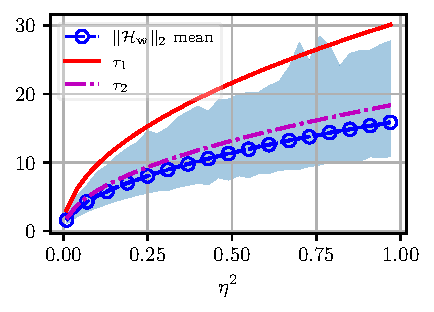
\includegraphics[width = \linewidth]{Figuras/taus_N_64_beta_0.9.pdf}
			\caption{$n = 64$}
		\end{subfigure}
		\begin{subfigure}{0.4\linewidth}
			\centering
			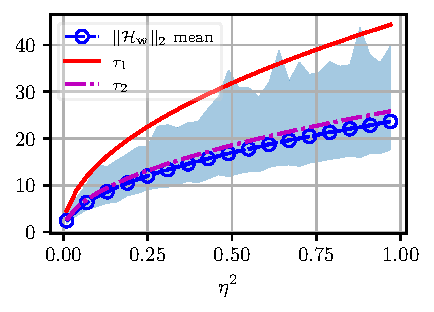
\includegraphics[width = \linewidth]{Figuras/taus_N_128_beta_0.9.pdf}
			\caption{$n = 128$}
		\end{subfigure}
		\begin{subfigure}{0.4\linewidth}
			\centering
			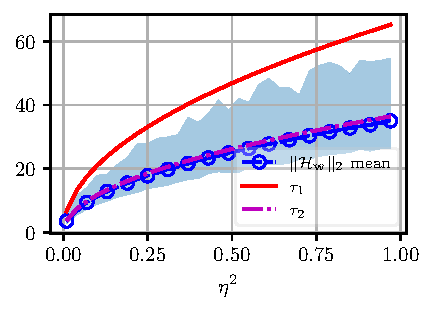
\includegraphics[width = \linewidth]{Figuras/taus_N_256_beta_0.9.pdf}
			\caption{$n = 256$}
		\end{subfigure}
		\begin{subfigure}{0.4\linewidth}
			\centering
			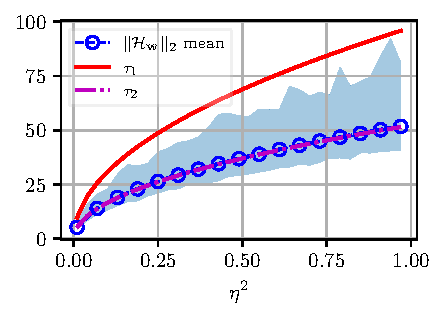
\includegraphics[width = \linewidth]{Figuras/taus_N_512_beta_0.9.pdf}
			\caption{$n = 512$}
		\end{subfigure}
		\caption{Realizaciones de $\|\Hank_\w\|_2$ y cotas $\tau_1$ y $\tau_2$ para diferentes dimensiones $n$ con $\beta = 0.9$}
		\label{fig:taus11}
	\end{figure}



	 
	
	\section{Criterio de información Bayesiana usando aproximación de Laplace ($BIC-lp$)}\label{BIC_Appendix}
	
	Una técnica muy empleada para estimar el orden del modelo son los criterios de la información \cite{Stoica2004}. Entre los más conocidos se encuentran el Criterio de información de Akaike, MDL, así como enfoques más reciente desarrollados en \cite{Mariani2015, Nielsen2013}, que garantizan un buen desempeño en el caso asintótico. Sin embargo, para registros de datos pequeños, estos métodos ya no son óptimos y su desempeño se ve deteriorada a medida que disminuye la relación señal a ruido (SNR). En \cite{Nielsen2013}, se propone un enfoque Bayesiano que tiene en cuenta el modelo de suma de exponenciales. A continuación se resume esta técnica
	
	Se observan los siguientes datos
	\begin{equation}
		\y = \begin{bmatrix} y_0 & y_1 & \cdots & y_{N-1}
		\end{bmatrix}^T
		\label{eq:BIC1}
	\end{equation}
	que se originaron a partir de un modelo desconocido. Como el modelo real no se conoce, se propone un conjunto de $K$ modelos paramétricos $\setM_1,\setM_2,\ldots,\setM_K$ tal que
	\begin{equation}
		\setM_k\quad : \quad \y = \matZ(\vecomega_k)\vecalpha_k + \w,
		\label{eq:BIC2} 
	\end{equation}
	donde $\w\sim\NormalC(\mathbf{0},\sigma^2\matI)$. Los diversos modelos candidatos difieren en términos de $\ell_k$, la cantidad de parámetros en $\vecalpha_k$. La matriz $\matZ(\vecomega_k)$ tiene dimensiones $N\times \ell_k$ y se puede asumir conocida como desconocida.
	
	El criterio de información Bayesiana (BIC) es una de las reglas de selección de modelo más  exitosas \cite{Stoica2005}. Para el modelo en \eqref{eq:BIC2}, el BIC se basa en un aproximación de la verosimilitud logaritmica
	\begin{equation}
		\ln p(\y \mid \setM_k) = -N\ln(\hat{\sigma}^2) - \ln(|\hat{\setI}_k|) + \mathcal{O}(1)
		\label{eq:BIC3} 
	\end{equation}
	donde $\hat{\sigma}^2$ es el estimador de máxima verosimilitud de la varianza de ruido, y $\hat{\setI}_k$ es la matriz de Fisher observada.
	
	Cada modelo $\setM_k$ está parametrizado por los parámetros del modelo $\vectheta = [\vecalpha_k^T\ \vecomega_k^T\ \sigma^2]$. La relación entre los datos $\y$ y el modelo $\setM_k$ viene dado por la función de probabilidad $p(\y\mid \vectheta_k,\setM_k)$. Existen diversas formas del BIC que surgen al ignorar términos de primer orden y considerar el comportamiento de $\hat{\setI}_k$ para varios valores de $N$ y $\hat{\sigma}^2$, así como la estructura de la matriz $\matZ(\vecomega_k)$. 
	
	En el marco Bayesiano, los parámetros desconocidos se consideran variables aleatorias. De modo que además de especificar una distribución para el ruido, también se tienen que obtener distribuciones a priori para los parámetros desconocidos, $p(\vectheta_k\mid\setM_k)$ con cierta probabilidad $p(\setM_k)$. Después de observar los datos, se obtienen la distribuciones a posterioris $p(\vectheta_k\mid\y,\setM_k)$ y $p(\setM_k\mid\y)$.
	
	\begin{equation}
		p(\vectheta_k\mid\y,\setM_k) = \frac{p(\y\mid\vectheta_k,\setM_k)p(\vectheta_k\mid\setM_k)}{p(\y\mid\setM_k)},
		\label{eq:Bic4} 
	\end{equation}
	\begin{equation}
		p(\setM_k\mid \y) = \frac{p(\y\mid\setM_k)p(\setM_k)}{p(\y)},
		\label{eq:BIC5}
	\end{equation}
	donde 
	\begin{equation}
		p(\y\mid\setM_k) = \int_{\vectheta_k} p(\y\mid\vectheta_k,\setM_k)p(\vectheta_k\mid\setM_k)\mathrm{d}\vectheta_k
		\label{eq:BIC6}
	\end{equation}
	es la función de verosimilitud. Para estimar el modelo, se comparan las probabilidad de dos modelos distintos $\setM_j$ y $\setM_i$. Es este sentido se definen las probabilidades a posteriori para los modelos como 
	\begin{equation}
		\frac{p(\setM_j\mid \y)}{p(\setM_i\mid \y)} = \mathrm{BF}[\setM_j,\setM_i]\frac{p(\setM_j)}{p(\setM_i)}.
		\label{eq:BIC7}
	\end{equation}
	donde 
	\begin{equation}
		\mathrm{BF}[\setM_j;\setM_i] = \frac{p(\y\mid\setM_j)}{p(\y\mid\setM_i)} = \frac{m_j(\y)}{m_i(\y)},
		\label{eq:BIC8}	
	\end{equation}
	se conoces como factor de Bayes, y $m_k(\y)$ es la verosimilitud marginal. Reescribiendo la distribución a posteriori del modelo en termino del factor de Bayes, se obtiene  
	\begin{equation}
		p(\setM_k\mid\y) = \frac{\mathrm{BF}[\setM_k,\setM_b]p(\setM_k)}{\sum_{i=1}^{K}\mathrm{BF}[\setM_i,\setM_b]p(\setM_i)}
		\label{eq:BIC9}
	\end{equation}
	donde $\setM_b$ es un modelo seleccionado para compara los otros modelos. Por lo tanto, el modelo más probable se encuentra maximizando $\mathrm{BF}[\setM_k; \setM_N ]$ sobre k, donde $\setM_N$ es el modelo de solo ruido ($\ell_k=0$).
	
	En \cite{Nielsen2013} se propone un nuevo BIC donde no es necesario investigar el comportamiento de la matriz de Fisher. Esta mejora es consecuencia del uso de un marco completamente Bayesiano en donde se obtienen distribuciones a priori adecuadas para los parámetros lineales. Como la dimensión del vector $\vecalpha_k$ varía entre los diferentes modelos, una distribución a priori adecuada viene dada por \cite{Zellner88}
	\begin{equation}
		\boldsymbol{\alpha}_k\mid \sigma \sim \mathcal{CN}(0,g\sigma[\matZ^H(\boldsymbol{\omega})\matZ(\boldsymbol{\omega})]^{-1})
		\label{eq:BIC10}
	\end{equation}
	Luego, la distribución a posteriori del parámetro $\vecalpha_k$ es
	\begin{equation}
		p(\vecalpha_k\mid \y, \sigma) \propto \exp\bigg[-(\vecalpha_k-\bar{\vecalpha}_k)^H\Sigmab^{-1}(\vecalpha_k-\bar{\vecalpha}_k)\bigg]
	\end{equation}
	donde
	\begin{equation}
		\Sigmab = \frac{g\sigma^2}{1+g}[\matZ^H(\vecomega_k)\matZ(\vecomega_k)]^{-1},
	\end{equation}
	\begin{equation}
		\bar{\vecalpha}_k = \frac{g}{1+g}\hat{\vecalpha}_k.
	\end{equation}
	Donde $\hat{\vecalpha}_k$ es el estimador de maxima verosimilitud de $\vecalpha_k$. El parámetro $g$ determina intuitivamente cuanto contribuye la distribución a priori de $\vecalpha_k$ a la distribución a posteriori. Por ejemplo si $g=0$, la media de la distribución a posteriori se reduce por completo a la media de la distribución a posteriori; si $g=1$ la media de la distribución a posteriori se reduce a $0.5$ de la media de la a priori. Si $g\to\infty$, la distribución a priori es una distribución no informativa. Si el parámetro $g$ está fijo pero es desconocido, su valor debe seleccionarse con cuidado. También puede tratarse como una variable aleatoria e integrarse a partir de la probabilidad marginal. Se suele utilizar una distribución beta invertida como a priori para $g$. Para el caos de los parámetros no lineales $\vecomega_k$ se suele utilizar una distribución a priori uniforme.
	
	Luego, la función de verosimilitud es
	\begin{equation}
		\begin{aligned}
			p(\y\mid\setM_k) = \int_{0}^\infty \int_{0}^\infty \int_{A_k} & p(\y\mid\vecalpha_k,\vecomega_k,\sigma^2,\setM_k)p(\vecalpha_k\mid g,\sigma^2,\vecomega_k,\setM_k) \times \\& \times p(\sigma^2)p(g)p(\vecomega_k\mid\setM_k)\mathrm{d}\vecalpha_k\mathrm{d}\vecomega_kdgd\sigma^2
		\end{aligned} \label{eq:BIC11}
	\end{equation}
	donde $A_k$ es un conjunto de dimensión $2k$ de números complejos.
	
	Desde un punto de vista computacional puede no ser ventajoso realizar la integral \eqref{eq:BIC11}. En cambio, la aproximación de Laplace se puede utilizar como una alternativa simple. Haciendo la aproximación de Laplace para la parametrización $\tau = \ln g$, se puede demostrar que el factor de Bayes del $BIC-lp$ es \cite{Nielsen2013}
	\begin{equation}
		\mathrm{BF}[\setM_k,\setM_N] = \int_{-\infty}^{\infty}\int_{A_k}q(\vecomega_k,\tau)\mathrm{d}\vecomega_k\mathrm{d}\tau
	\end{equation}
	donde el integrando está dado por
	\begin{equation}
		q(\vecomega_k,\tau) = \mathrm{BF}[\setM_k;\setM_N\mid \exp(\tau),\vecomega_k]p(\vecomega_k\mid\setM_k)p(\tau)
		\label{eq:BIC12}
	\end{equation}
	con
	\[p(\tau) = \exp(\tau)p(\exp(\tau)\mid\delta).\]
	Usando la aproximación de Laplace
	\begin{equation}
		\mathrm{BF}[\setM_k,\setM_N] \approx \int_{-\infty}^{\infty} q(\hat{\vecomega}_k,\tau)(2\pi)^{\rho_k/2-1}\big|\mathbf{H}(\hat{\vecomega}_k)\big|^{-1/2}\mathrm{d}\tau.
		\label{eq:BIC13} 
	\end{equation}
	donde 
	\begin{equation}
		\mathbf{H}(\vecomega_k) = \frac{\partial^2\ln q(\vecomega_k,\tau)}{\partial\vecomega_k\partial\vecomega_k^T}, 
		\label{eq:BIC14}
	\end{equation}
	
	Entonces, el modelo con la probabilidad posterior más alta es la solución a
	\begin{equation}
		\begin{aligned}
			\hat{k} = \arg\max &\big[ -N\ln\big(\y^H(\matI_N-\frac{g}{g+1}\matP_\matZ)\y\big)-\ell_k\ln(1+\hat{g})\\ & +  \ln\hat{g} - \delta\ln(1+\hat{g}) + (2\ell_k+1)2\pi + \frac{1}{2}\ln(\gamma(\hat{g}\mid\vecomega_k)) - \frac{1}{2}\ln|\mathbf{H}(\vecomega_k)|\big].
		\end{aligned}
		\label{Eq:BIC15}
	\end{equation}
	
	Donde 
	
	\[\matP_\matZ = \matZ(\boldsymbol{\omega}_k)\big(\matZ^H(\boldsymbol{\omega}_k)\matZ(\boldsymbol{\omega}_k)\big)^{-1}\matZ^H(\boldsymbol{\omega}_k)\]
	\[R^2 = \frac{\y^H\matP_\matZ\y}{\y^H\y}\]
	
	\[\hat{g} = \exp\hat{\tau}\]
	\[\hat{\tau} = \ln\bigg(\frac{\beta_\tau + \sqrt{\beta_\tau^2 - 4\alpha_\tau}}{-2\alpha_\tau}\bigg)\]
	\[\beta_\tau = (N/r-1)R^2 + 2 + (N-\ell_k-\delta)/r - N/r,\]
	\[\alpha_\tau = (1-R^2)(1+(N-\ell_k-\delta)/r - N/r)\]
	\[\gamma(\hat{g}\mid\boldsymbol{\omega}_k) = \bigg[\frac{\hat{g}(N/r)(1-R^2)}{[1+\hat{g}(1-R^2)]^2}-\frac{\hat{g}(N-\ell_k-\delta)/r}{(1+\hat{g})^2}\bigg]\]
	
	
	   \newpage
	
	\section*{Apéndice}
	\addcontentsline{toc}{section}{\bfseries Appendices}
	\renewcommand{\thesubsection}{\arabic{subsection}}
	\setcounter{subsection}{0}
	
	\subsection{Lemas y definiciones auxiliares}
	
	Para demostrar los resultados obtenidos en este capítulo serán útiles los siguiente resultados.
	\begin{lemma}
		$\setX = \setY$ si y solo si $\Thetab(\setX,\setY) = \mathbf{0}$
	\end{lemma}
	\begin{proof}
		Por construcción, los vectores $\{\x_1,\ldots,\x_s\}$ forman un base del subespacio $\setX$. De igual forma $\{\y_1,\ldots,\y_s\}$ es una base $\setY$. Si $\cos\theta_k=1$, se tiene que $\x_k$ e $\y_k$ están alineados. Por lo tanto, si todos los ángulos principales son cero, los conjuntos  $\{\x_1,\ldots,\x_s\}$ y $\{\y_1,\ldots,\y_s\}$ generan el mismo subespacio.
		
		Por otro lado, cuando $\setX=\setY$, es claro que 
		\[\max_{\stackrel{\x\in\setX}{\y\in\setY}}\frac{|\langle\x,\y\rangle|}{\|\x\|_2\|\y\|_2} = 1\]
		y por lo tanto, $\cos\theta_k = 1$ para todo $k$.
	\end{proof}
	
	\begin{definition}
		La distancia entre los subespacios $\setX$ e $\setY$ está dada por
		\begin{equation}
			\rho(\setX,\setY) = \max\bigg\{\max_{\stackrel{\x\in\setX}{\|\x\|_2=1}}\dist(\x,\setY),\max_{\stackrel{\y\in\setY}{\|\y\|_2=1}}\dist(\y,\setX) \bigg\}
			\label{Eq:GapDistance}
		\end{equation}
	\end{definition}
	
	\begin{prop}\label{Prop:GapDistance}
		Sean $\setX$ e $\setY$ dos subespacio, se definen $\matProj_{\setX}$ y $\matProj_{\setY}$ la proyección ortogonal sobre $\setX$ e $\setY$ respectivamente. Luego,
		\begin{itemize}
			\item[i)] $\rho(\setX,\setY) = \|\matProj_{\setX}-\matProj_{\setY}\|_2$
			\item[ii)] $\rho(\setX,\setY)=\sin\theta_1$, con $\theta_1$ es el máximo ángulo principal entre $\setX$ e $\setY$.
		\end{itemize} 
	\end{prop}
	\begin{proof}
		La demostración de esta proposición está en \cite[Teorema 4.5]{Stewart1990}
	\end{proof}
	

	
	
	
	

